\documentclass[12pt,twocolumn]{scrartcl}
\usepackage[utf8x]{inputenc}
\usepackage[ngerman]{babel}

\newcommand{\studenta}{Alex Baumgärtner, Annalena Gutheil, Benjamin Weißer,}
\newcommand{\studentb}{Paul Pasler, Daniel Andrés López}

\newcommand{\reporttitle}{Using the soundwave doppler effect to sense gestures}  
\newcommand{\reportsubtitle}{Exposé}

\newcommand{\handoverdate}{16.12.2013}

\newcommand{\reportsemester}{WS 2013/14}
\newcommand{\degree}{Master of Science}
\newcommand{\universitys}{HSRM}
\newcommand{\university}{Hochschule RheinMain}
\newcommand{\studiengang}{Informatik}
\newcommand{\prof}{Prof. Dr. U. Schwanecke} 

\newcommand{\listingssetup}{
	\lstset{
		language=Python,                % the language of the code
		basicstyle=\footnotesize,       % the size of the fonts that are used for the code
		numbers=left,                   % where to put the line-numbers
		numberstyle=\tiny\color{gray},  % the style that is used for the line-numbers
		stepnumber=0,                   % the step between two line-numbers. If it's 1, each line 
		                                % will be numbered
		numbersep=5pt,                  % how far the line-numbers are from the code
		backgroundcolor=\color{white},  % choose the background color. You must add \usepackage{color}
		showspaces=false,               % show spaces adding particular underscores
		showstringspaces=false,         % underline spaces within strings
		showtabs=false,                 % show tabs within strings adding particular underscores
		frame=single,                   % adds a frame around the code
		rulecolor=\color{black},        % if not set, the frame-color may be changed on line-breaks within not-black text (e.g. commens (green here))
		tabsize=2,                      % sets default tabsize to 2 spaces
		captionpos=b,                   % sets the caption-position to bottom
		breaklines=true,                % sets automatic line breaking
		breakatwhitespace=false,        % sets if automatic breaks should only happen at whitespace
		title=\lstname,                 % show the filename of files included with \lstinputlisting;
		                                % also try caption instead of title
		keywordstyle=\color{blue},      % keyword style
		commentstyle=\color{green},     % comment style
		stringstyle=\color{gray},       % string literal style
		escapeinside={\%*}{*)},         % if you want to add LaTeX within your code
		morekeywords={*,...}            % if you want to add more keywords to the set
	}
}


\usepackage{lipsum}
\usepackage{fancyhdr} 
%\usepackage{scrpage2}
\usepackage[font=small]{caption}
\usepackage{calc}
\usepackage{xcolor}
\usepackage{setspace}
\usepackage{pdfpages}
\usepackage{enumerate}
\usepackage{scrhack}
\usepackage[pdftex,pdfborder={0 0 0}, bookmarksopenlevel=1,
bookmarksdepth=3]{hyperref} %Kreiert Links von der Table of Content zu Kapiteln (ohne optische Hervorhebung)

\usepackage[]{acronym}
\usepackage{graphicx}
\usepackage{subfigure}
\usepackage{wrapfig}

\usepackage{tikz}
\usetikzlibrary{trees}
 
\usepackage{hhline} %% extended line features for tables with \hhline{}
\usepackage{multirow} %% merges several cells over rows: \multirow{Zeilen}{Breite}{Inhalt}; over columns: \multicolumn{Spalten}{Ausrichtung}{Inhalt}
\usepackage{colortbl} %% use defined colors in tables
\usepackage{booktabs} %% better horizontal lines in tables with \toprule[<breite>], \midrule[<breite>], \cmidrule[<breite>](trim){a-b}, \bottomrule 
\usepackage{supertabular}
\usepackage{longtable}
\usepackage{rotating} 
\usepackage{makecell}
\usepackage{pict2e}

\usepackage{chngcntr}
\usepackage{float}
\newfloat{listing}{htbp}{scl}
\floatname{listing}{Listing}
\usepackage{listings} 
	\definecolor{grey1}{rgb}{0.95,0.95,0.95}
	\DeclareCaptionFont{white}{\color{white}}
	\DeclareCaptionFormat{listing}{\colorbox{gray}{\parbox{\columnwidth}{#1#2#3}}}
	\captionsetup[lstlisting]{format=listing,labelfont=white,textfont=white}
	\renewcommand\lstlistingname{Quelltext}
	\renewcommand\lstlistlistingname{Quelltexte}  
	\lstset{
		language=Python,
		basicstyle=\ttfamily\footnotesize,
		numbers=left,
		% numberstyle=\tiny\color{gray}, 
		stepnumber=1,
		numbersep=3pt,
		backgroundcolor=\color{grey1},
		showspaces=false,
		showstringspaces=false,
		showtabs=false,
		frame=tb,
		rulecolor=\color{black},
		tabsize=1,
		captionpos=t,
		breaklines=true,
		breakatwhitespace=false,
		title=\lstname,
		keywordstyle=\color{blue},
		commentstyle=\color{darkgreen},
		stringstyle=\color{gray},
		escapeinside={\%*}{*)},
		morekeywords={*,...},
		xleftmargin=20pt,
		framexleftmargin=20pt,
		framexrightmargin=6pt
	}
	\lstset{literate=
		{Ö}{{\"O}}1
		{Ä}{{\"A}}1
		{Ü}{{\"U}}1
		{ß}{{\ss}}2
		{ü}{{\"u}}1
		{ä}{{\"a}}1
		{ö}{{\"o}}1
	}
 \AtBeginDocument{
	\renewcommand{\subsectionautorefname}{\sectionautorefname}
	\renewcommand{\subsubsectionautorefname}{\sectionautorefname}
	\renewcommand{\figureautorefname}{Abbildung}
	\renewcommand{\figurename}{Abb.}
	\renewcommand{\tableautorefname}{Tabelle}
	\renewcommand{\equationautorefname}{Formel}
	\counterwithin{equation}{section}
	\counterwithin{lstlisting}{section}
	\counterwithin{figure}{section}
	\counterwithin{table}{section}
	\renewcommand{\thelstlisting}{\thesection.\arabic{lstlisting}}
 }	

\hypersetup{
	pdftitle=\reporttitle\ - \students ,
	pdfauthor=\students , 
	pdfsubject=\reporttitle ,
	pdfkeywords=\universitys 
}

\newcommand{\settocdepth}[1]{
	\addtocontents{toc}{
		\protect
		\setcounter{tocdepth}{#1}
	}
}

\newcommand{\head}[1] {
 	\lhead{\ifthispageodd{}{#1}}
 	\rhead{\ifthispageodd{#1}{}}
 }

\newcommand{\headAndToc}[1] {
	\head{#1}
	\addcontentsline{toc}{section}{#1}
}

\definecolor{darkblue}{rgb}{0, 0, .5}
\definecolor{darkgreen}{rgb}{0, .5, 0}
\definecolor{lightgray}{rgb}{.7, .7, .7}
\definecolor{darkgray}{rgb}{.4, .4, .4}

%% math
\usepackage{amsmath,amssymb,amsfonts}
\newcommand{\Z}{\mathbb{Z}}
\newcommand{\order}{\mathrm{order\:}}
\newcommand{\IV}{\mathrm{IV}}
\newcommand{\tmod}{\!\!\mod}

\renewcommand\sectionmark[1]{
  \def\sectionname{#1}
  \markright{\thesection #1}
} 
  
\renewcommand\subsectionmark[1]{
  \def\subsectionname{#1}
  \markright{\thesubsection #1}
} 
	
\graphicspath{{./ref/images/}}

\newlength{\iconwidth}
\setlength{\iconwidth}{1cm}
\definecolor{boxheadcol}{gray}{.6}
\definecolor{boxcol}{gray}{.9}
\newenvironment{xlist}[1]{%
  \begin{list}{}{%
    \settowidth{\labelwidth}{#1:}
    \setlength{\labelsep}{0.5cm}
    \setlength{\leftmargin}{\labelwidth}
    \addtolength{\leftmargin}{\labelsep}
    \setlength{\rightmargin}{0pt}
    \setlength{\parsep}{0.5ex plus 0.2ex minus 0.1ex}
    \setlength{\itemsep}{0 ex plus 0.2ex}
    \renewcommand{\makelabel}[1]{##1:\hfil}
    }
  }
{\end{list}}


\title{\pebericht}
\author{\student}
\date{\handoverdate}
\begin{document}
\pagestyle{fancy}  
% \pagestyle{scrheadings}
% \automark[section]{chapter}
\fancyhfoffset{\marginparsep}
\renewcommand{\footrulewidth}{1.0pt}
\renewcommand{\headrulewidth}{1.0pt}
\renewcommand{\headheight}{30pt}

\setlength{\parindent}{0in}
\setlength{\parskip}{0.5em}
\clubpenalty 10000
\widowpenalty 10000

\chead{}
\cfoot{}
 
\lfoot{\ifthispageodd{}{\thepage}}	
\rfoot{\ifthispageodd{\thepage}{}}

\pagenumbering{Roman}

\pdfbookmark[1]{Titelseite}{titlepage}
\begin{titlepage} 
	\begin{center}

	\vspace{2.2cm}
	{\large \textbf{\university}}\\
	\vspace{2cm}
	
	\includegraphics*[width=4.5cm]{hsrmlogo}\\
	\vspace{2.8cm}	
	{\small Machine Learning}\\ 
	\vspace{1cm}
	\doublespacing
	{\Huge \textbf{\reporttitle}}\\ 
	\singlespacing 
	\vspace{1cm}
	{\large \reportsubtitle}\\ 
	\vspace{2.2cm}
	\onehalfspacing
	  
	\begin{tabbing}
		xxxxxxxxxxxxxxxx\=xxxxxxxxxxxxxxxxxxxxxxx\kill
		Namen: \> {\textbf{\studenta}} \\
		\>  \textbf{\studentb}\\
		{Matrikelnummern}: \> \matrikel \\
		Studiengang: \> \studiengang, \degree\\
		Studiengangsleiter: \> \prof \\
		{Semester}: \> \reportsemester  \\
		{Datum:} \> \handoverdate \\
	\end{tabbing}
	\singlespacing 

\end{center}  

\end{titlepage} 
 
\clearpage


\phantomsection
\headAndToc{Inhaltsverzeichnis}
\begin{spacing}{1}
\tableofcontents
\end{spacing}
\clearpage
\singlespacing
 
\setcounter{table}{0}
\setcounter{figure}{0}
\pagenumbering{arabic}
\lhead{\ifthispageodd{}{\nouppercase{\leftmark}}}
\rhead{\ifthispageodd{\rightmark}{}}
\section{Einleitung}
\label{sec:intro}
Eine Alternative zu den Standardeingabegeräten wie Maus und Tastatur zur
Interaktion mit Computern sind Gesten.
Von besonderem Interesse ist dabei das Erkennen von sogenannten \glqq
In-Air\grqq -Gesten, die mit den Händen in der Luft ausgeführt werden. Der
Unterschied zu Gesten, wie sie beispielsweise auf Touch-Displays von Smartphones
für das Rotieren oder Skalieren von Bildern verwendet werden, besteht darin,
dass die Interaktion kontaktfrei ist und durch die Bewegung der Hände im Raum
wesentlich komplexere Gesten realisiert werden können.

Zwei bekannte Geräte zur In-Air-Gestenerkennung sind \textit{Leap
Motion}~\cite{LeapMotion} und \textit{Microsoft Kinect}~\cite{Kinect}. Diese Geräte
verwenden optische Verfahren zur Erkennung der Hände oder Finger. Ein Nachteil
beider Verfahren ist jedoch, dass sie wegen der optischen Erkennung sehr
abhängig von der Beleuchtung sind. Weiterhin ist die Gesten-Erkennung erst durch
die Verwendung zusätzlicher Hardware möglich.

Ein alternativer Ansatz ist die Verwendung von Mikrofon und Lautsprecher zur
akustischen Erkennung von Gesten. Ein Vorteil dieses Ansatzes gegenüber Leap
Motion oder Microsoft Kinect ist, dass die meisten Computer und Laptops mit
dieser Hardware bereits ausgestattet sind.
Das in \cite{Gupta2012} beschriebene Verfahren nutzt dazu den Doppler-Effekt,
also die Frequenzverschiebungen eines konstanten Tons bei zeitlicher Veränderung
der Entfernung zwischen der Schallquelle (Sender) und dem Empfänger.
Über die Lautsprecher (Sender) wird ein konstanter, hochfrequenter Ton
ausgegeben, der von dem Mikrofon (Empfänger) aufgenommen wird.
Da sowohl Sender als auch Empfänger eine feste Position haben, kommt es durch
das Bewegen der Hände zu Frequenzverschiebungen, die sich auf den Doppler-Effekt
zurückführen lassen. 
Diese Frequenzverschiebungen können analysiert und Rückschlüsse auf die Richtung
und die Geschwindigkeit von der Bewegung gezogen werden.

% Ziel des Projektes ist es ein Programm zu entwickeln, was Gesten erkennt. Dazu
% wurde von Microsoft ein Verfahren entwickelt, welches anhand der Doppler
% Verschiebung, eines Soundsignals, Gesten erkennt. Dieses Verfahren wird in
% \cite{Gupta2012} beschrieben. Um die Gesten zu erkennen sollen verschiedene
% Machine Learning Verfahren verwendet werden.

Im Rahmen der Lehrveranstaltung Machine Learning an der Hochschule RheinMain im
Studiengang Master Informatik soll eine Anwendung mit dem Ziel entwickelt
werden, die akustische Erkennung und Klassifikation von Gesten auf Grundlage des
Doppler-Effekts durch verschiedene Machine Learning Verfahren zu realisieren.

Die Anwendung soll folgende Gesten unterscheiden können:
\begin{itemize}
	\item \texttt{\ac{RLO}}\\
	Das Bewegen der Hand von rechts nach links vor dem Bildschirm
	\item \texttt{\ac{TBO}}\\
	Das Bewegen der Hand von oben nach unten vor dem Bildschirm
	\item \texttt{\ac{OT}}\\
	Beide Hände entgegengesetzt auf den Bildschirm hin und weg bewegen
	\item \texttt{\ac{SPO}}\\
	Mit einer Hand eine kurze Bewegung in Richtung des Monitors und zurück
	\item \texttt{\ac{DPO}}\\
	Mit einer Hand zwei kurze aufeinander folgende Bewegungen in Richtung des Monitors und zurück
	\item \texttt{\ac{RO}}\\
	Rotation mit einer Hand
\end{itemize}

Zur Abgrenzung der Gesten zu einer Nicht-Geste werden zusätzlich noch die
Hintergrundgeräusche als Klasse definiert. Dies ist einmal \texttt{\ac{BNS}},
diese Geste spiegelt die Referenzfrequenz wieder, und zum Anderen
\texttt{\ac{BNN}}, bei dieser Geste herrscht zusätzlich noch beliebiger Lärm im
Raum.

\subsection{Klassifikationsverfahren}
Die Gestenerkennung soll anhand verschiedener Klassifikationsverfahren erfolgen.
Dabei müssen die Rohdaten unterschiedlich verarbeitet und auf verschiedene
Methoden angewendet werden, um eine Klassifikation zu erreichen. Es werden die
Vor- und Nachteile der unterschiedlichen verfahren auf das Projekt bezogen
diskutiert. Jedes Klassifikationsverfahren ist in einem Kapitel im Detail
beschrieben. Folgende fünf Verfahren werden in den Kapiteln untersucht:
\begin{itemize}
	\item \ref{mainsec:svm}. \nameref{mainsec:svm}
	\item \ref{mainsec:hmm}. \nameref{mainsec:hmm}
	\item \ref{mainsec:kmeans}. \nameref{mainsec:kmeans}
	\item \ref{mainsec:trees}. \nameref{mainsec:trees}
	\item \ref{mainsec:lstm}. \nameref{mainsec:lstm}
\end{itemize}


\subsection{Rahmenprogramm}
\label{sec:app}
Alle fünf Klassifikatoren nutzen ein gemeinsames Grundprogramm, welches die
gemeinsamen Aufgaben bewältigt. Das Programm ist in \texttt{Python} geschrieben
und ist für die Tonerzeugung und -aufnahme sowie für die allgemeine Steuerung
verantwortlich. 

Die Referenzfrequenz von 18,5 kHz wird kontinuierlich im Modul
\texttt{soundplayer.py} abgespielt. Mit dem Modul \texttt{recorder.py} werden
die Audiosignale mit einer Samplingrate von 48000 aufgenommen und mit Hilfe einer
Fouriertransformation zu einem Datenobjekt mit dem Frequenzspektrum im Bereich
von ~18 kHz bis ~19 kHz umgewandelt. Die so aufgenommenen Rohdaten werden
entweder bei der Aufnahme von Beispielen abgespeichert oder bei der Live
Klassifikation dem genutzten Klassifikator übergeben. Das aufgenommene Array des
Frequenzspektrums enthält 64 Werte. Dieses Array wird als \textit{Frame}
bezeichnet.

Des Weiteren wird das einheitliche Interface \texttt{IClassifier} für die
Klassifikatoren verwendet, um die Steuerung der einzelnen Klassifikatoren zu
vereinheitlichen. Diese können über eine integrierte Konsole angesteuert werden.
In der Konsole können über verschiedene Befehle die Live Klassifizierung, das
Training, eine Validierung etc. gestartet werden.
\enlargethispage{\baselineskip}
Die Konsole bietet auch die Möglichkeit Beispieldaten aufzunehmen. Eine
Beispielgeste besteht aus 32 aufeinanderfolgenden Frames. Die Aufnahme kann auch
im Batchverfahren direkt hintereinander erfolgen (mehrmals die gleiche Geste
ohne zusätzliche Interaktion). Aufgenommene Gesten werden pro Nutzer in
einzelnen Gesten-Ordnern gespeichert. Das Rahmenprogramm bietet auch eine
Schnittstelle zum Laden der Beispieldaten in ein NumPy Array. Dies wird im Modul
\texttt{gesturefileio.py} vorgenommen. Dabei können verschiedene Datenformate
geladen und auch schon eine einfache Normalisierung vorgenommen werden.



\clearpage
\section{Support Vector Machine}
\label{mainsec:svm}
\textit{Manuel Dudda, Benjamin Weißer}

Im Jahr 1958 veröffentlichte der Psycholge und Informatiker Frank Rosenblatt sein entwickeltes Konzept des Perzeptrons \cite{rosenblatt58a}. 
Die Idee entstammt der Neurobiologie und simuliert die Funktionsweise eines menschlichen Gehirns. 
Perzeptronen sind vereinfachte künstliche neuronale Netze, bestehend aus mehreren künstlichen Neuronen, die ein formales Modell einer Nervenzelle beschreiben. 
In der Grundversion besteht ein Perzeptron aus einem einzigen Neuron. 
Es verarbeitet einen Eingabevektor zu einer Ausgabe. 
Anhand eines Schwellwertes wird entschieden, ob das Neuron "{}feuert"{} oder nicht. 
Bei der Verarbeitung des Eingabevektors wird für jede Komponente eine Gewichtung berücksichtigt, sodass die Ausgabe auf gewisse Eingaben eingestellt werden kann. 
Mehrlagige Perzeptronen (\ac{MLP}) sind in der Lage, Eingabevektoren in Ausgabevektoren umzuwandeln. 

\begin{figure}[htbp] \centering
    \subfigure[AND-Pezeptron mit einem Neuron]{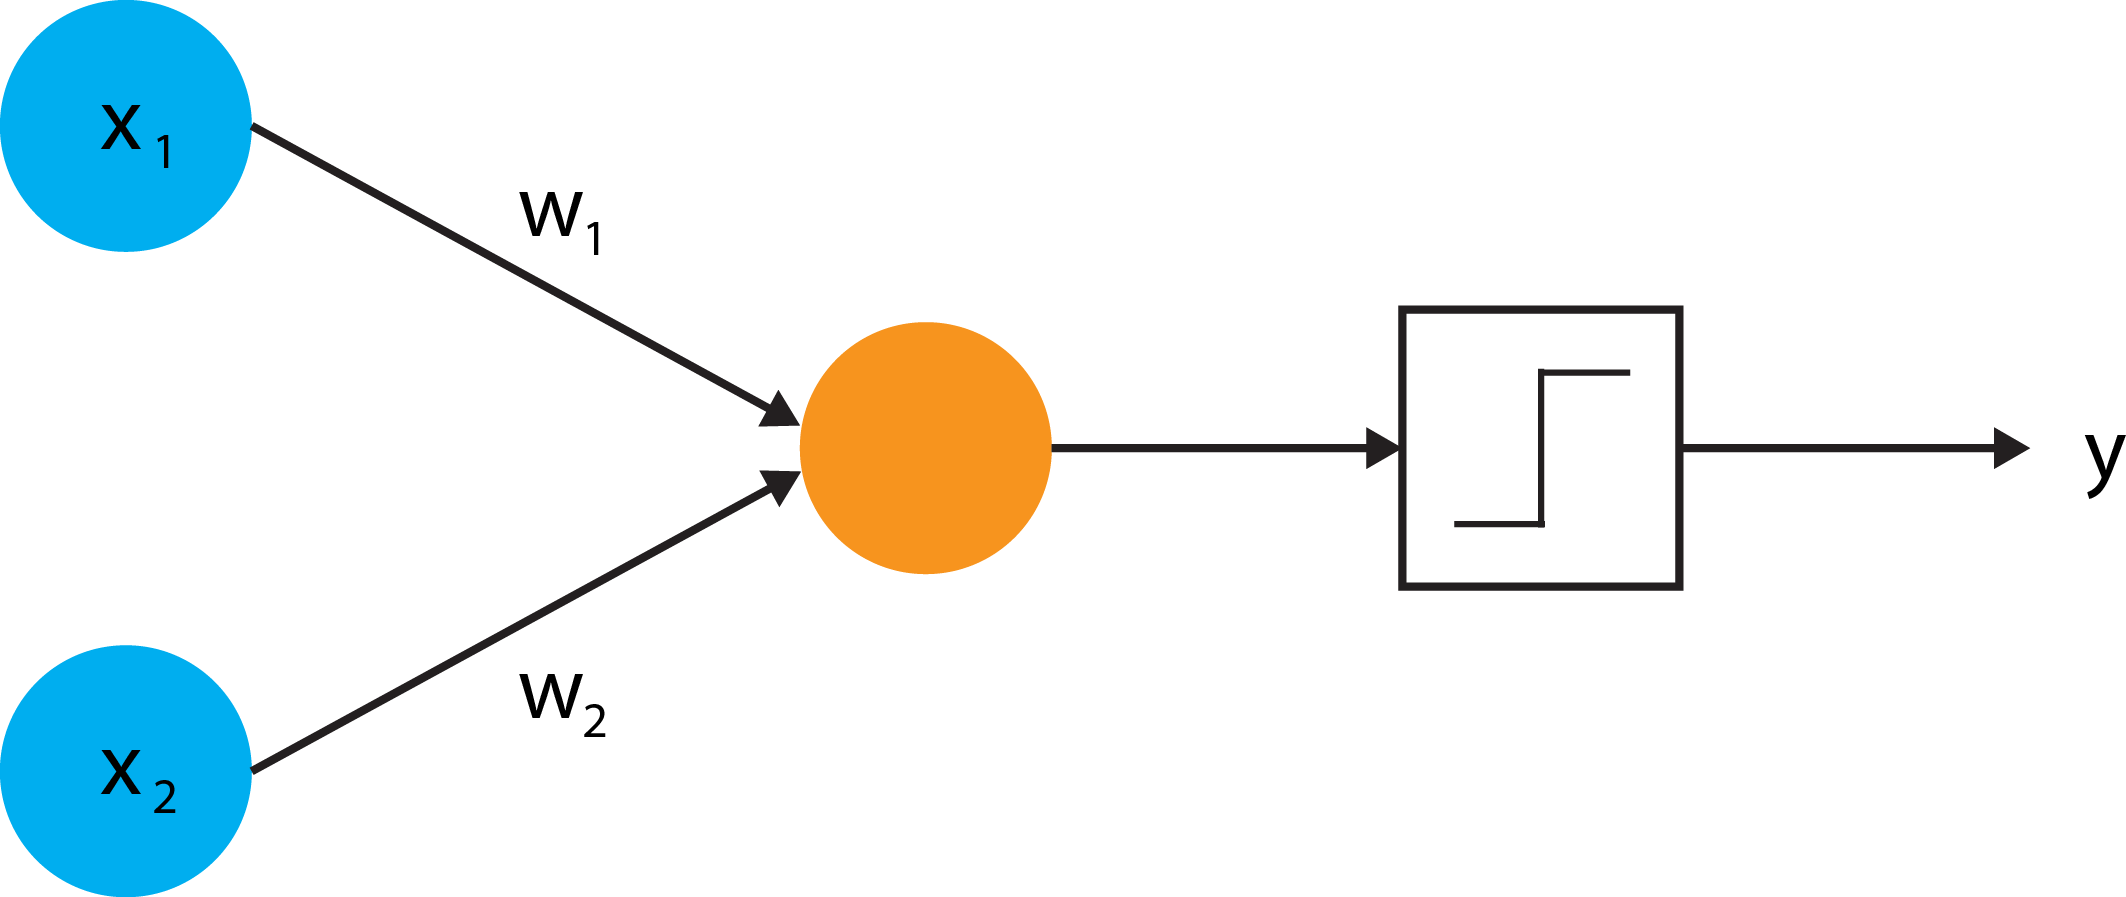
\includegraphics[width=0.23\textwidth]{svm/svm_perceptron.png}}
    \subfigure[AND linear separierbar in $\mathbb{R}^2$]{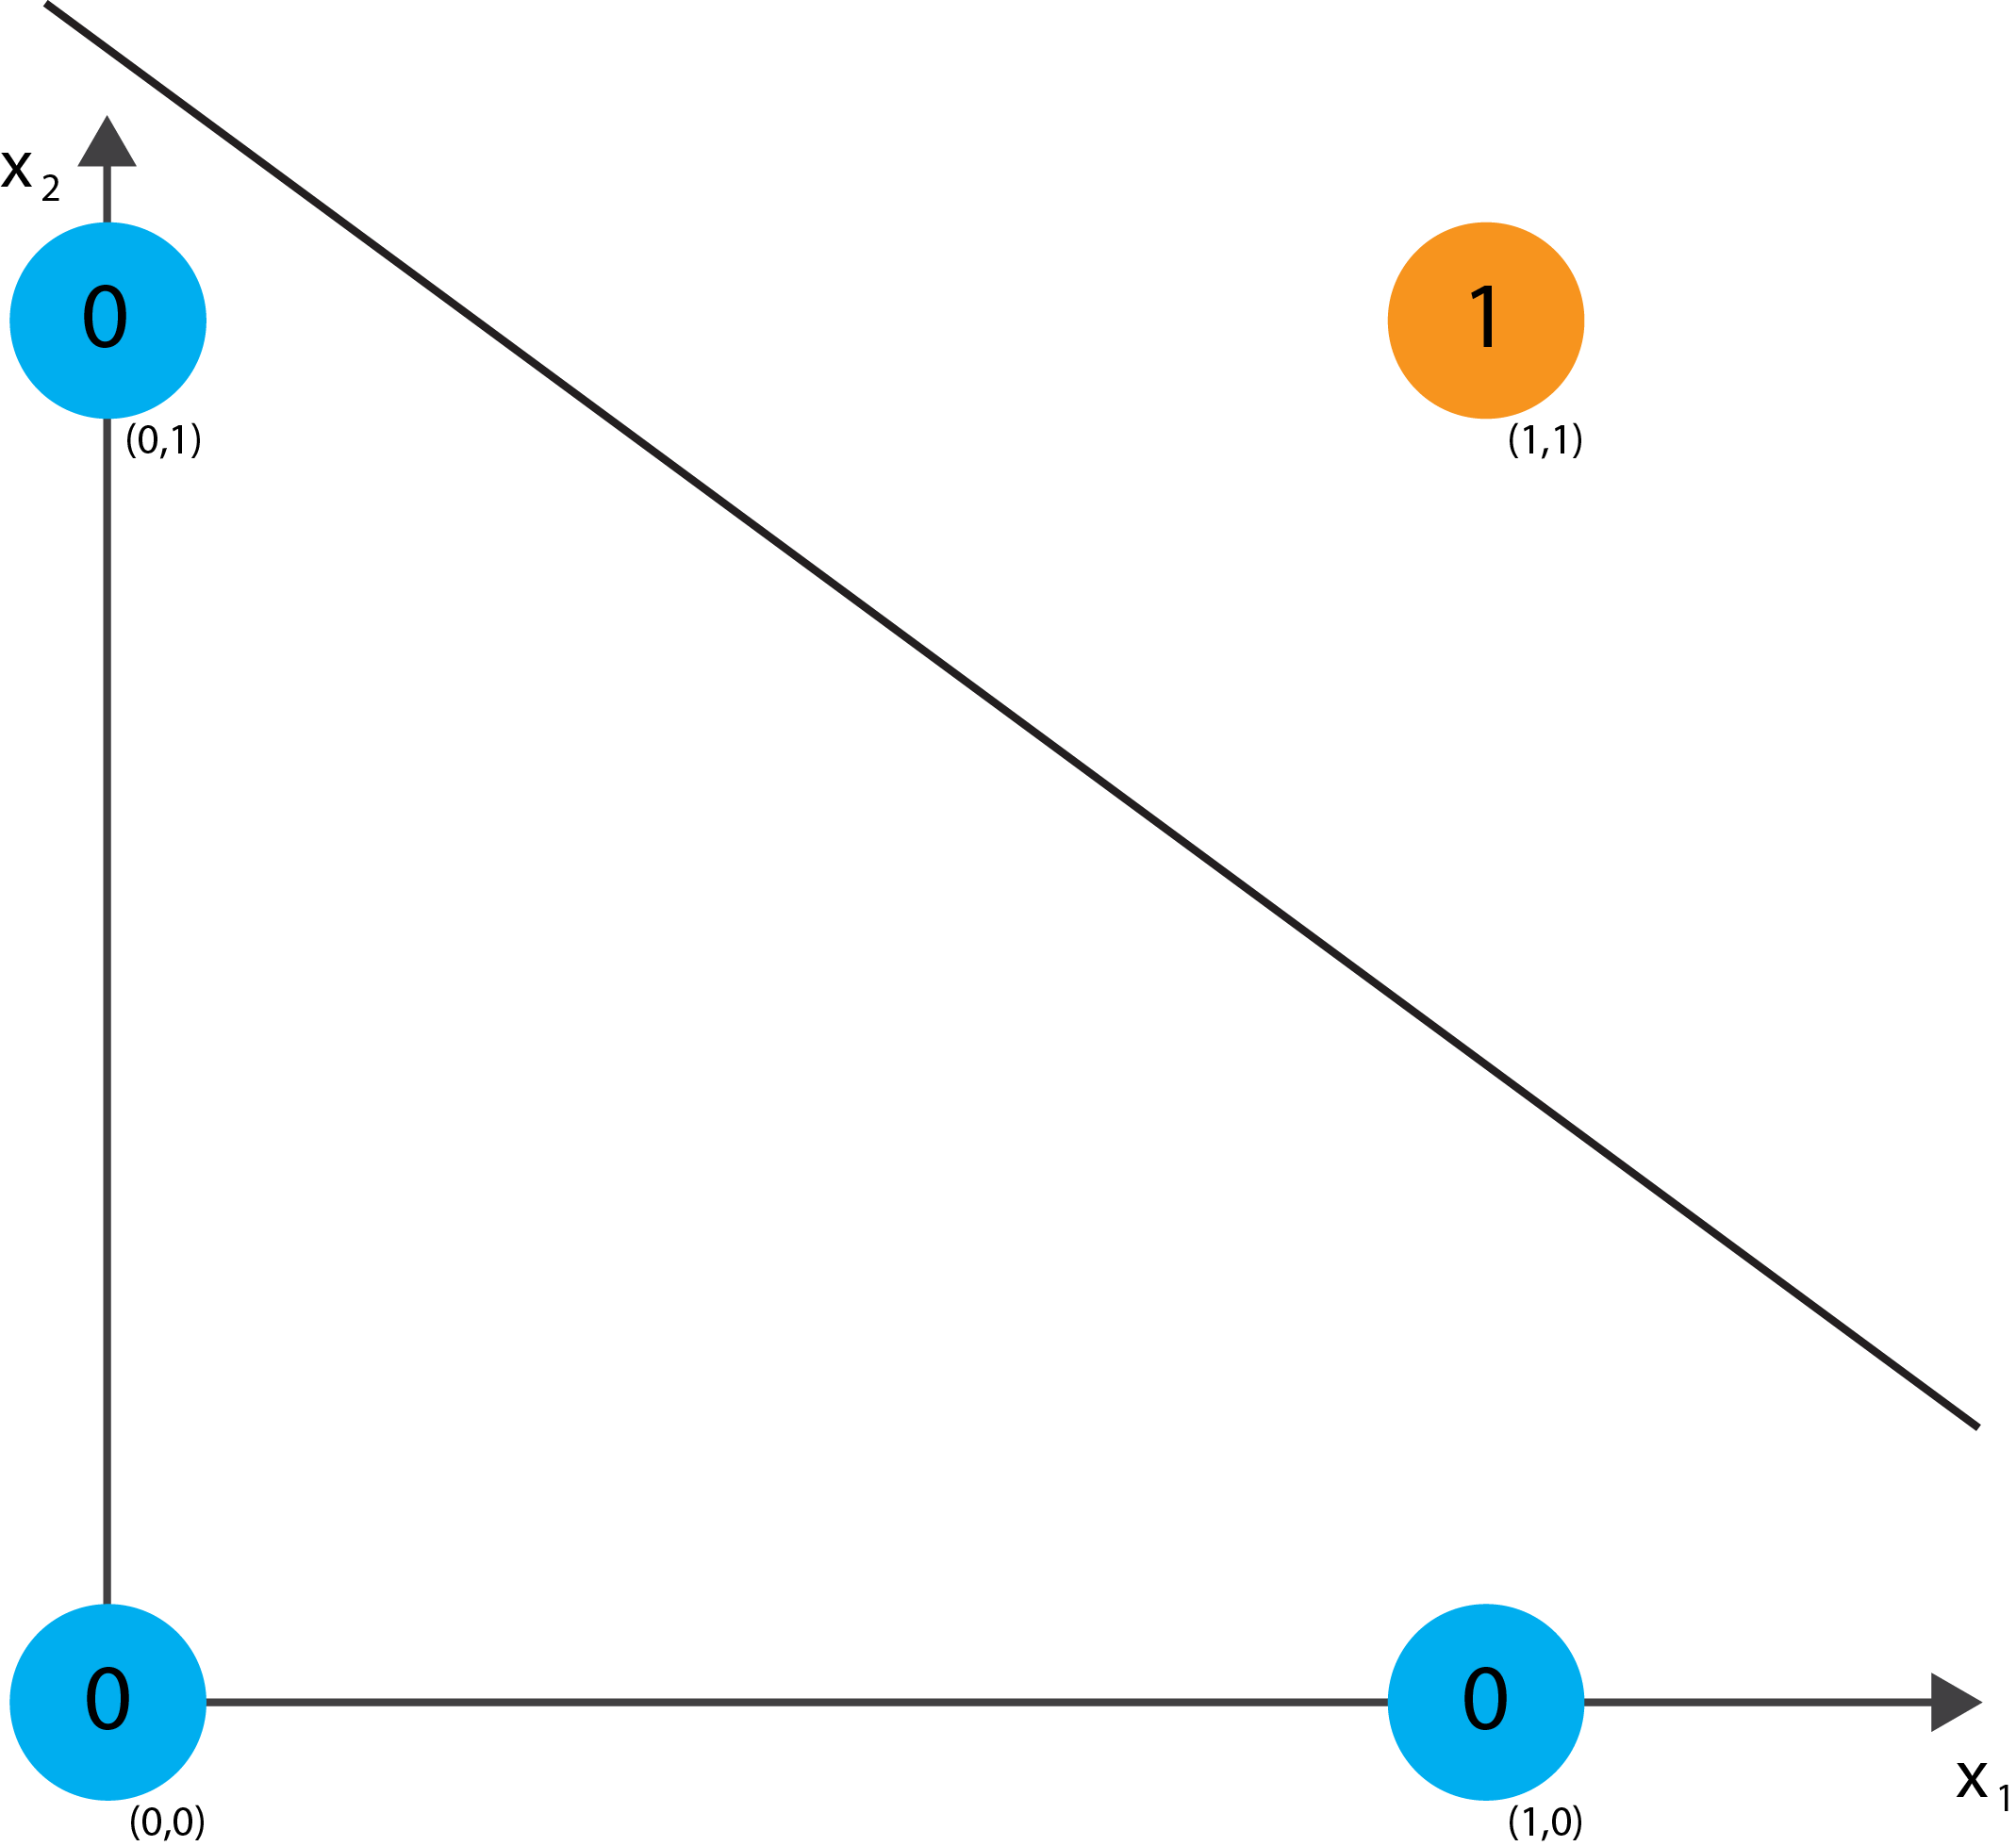
\includegraphics[width=0.23\textwidth]{svm/svm_and.png}}
    \caption{AND-Perzeptron}
    \label{fig:perceptron_and}
\end{figure}

Die jeweiligen Gewichtungen können so eingestellt werden, dass der Eingabevektor in einen bestimmten Ausgabevektor umgewandelt wird. 
Abb. \ref{fig:perceptron_and} zeigt, wie ein einfaches Perzeptron die AND-Funktion realisiert, und visualisiert die Klassifizierungsentscheidung in einem Koordinatensystem. 

Einlagige Perzeptronen sind beschränkt auf die Lösung linear separierbarer Probleme. 
Ein einfaches XOR kann also nicht realisiert werden (Abb. \ref{fig:perceptron_xor}). 

\begin{figure}[htbp] \centering
    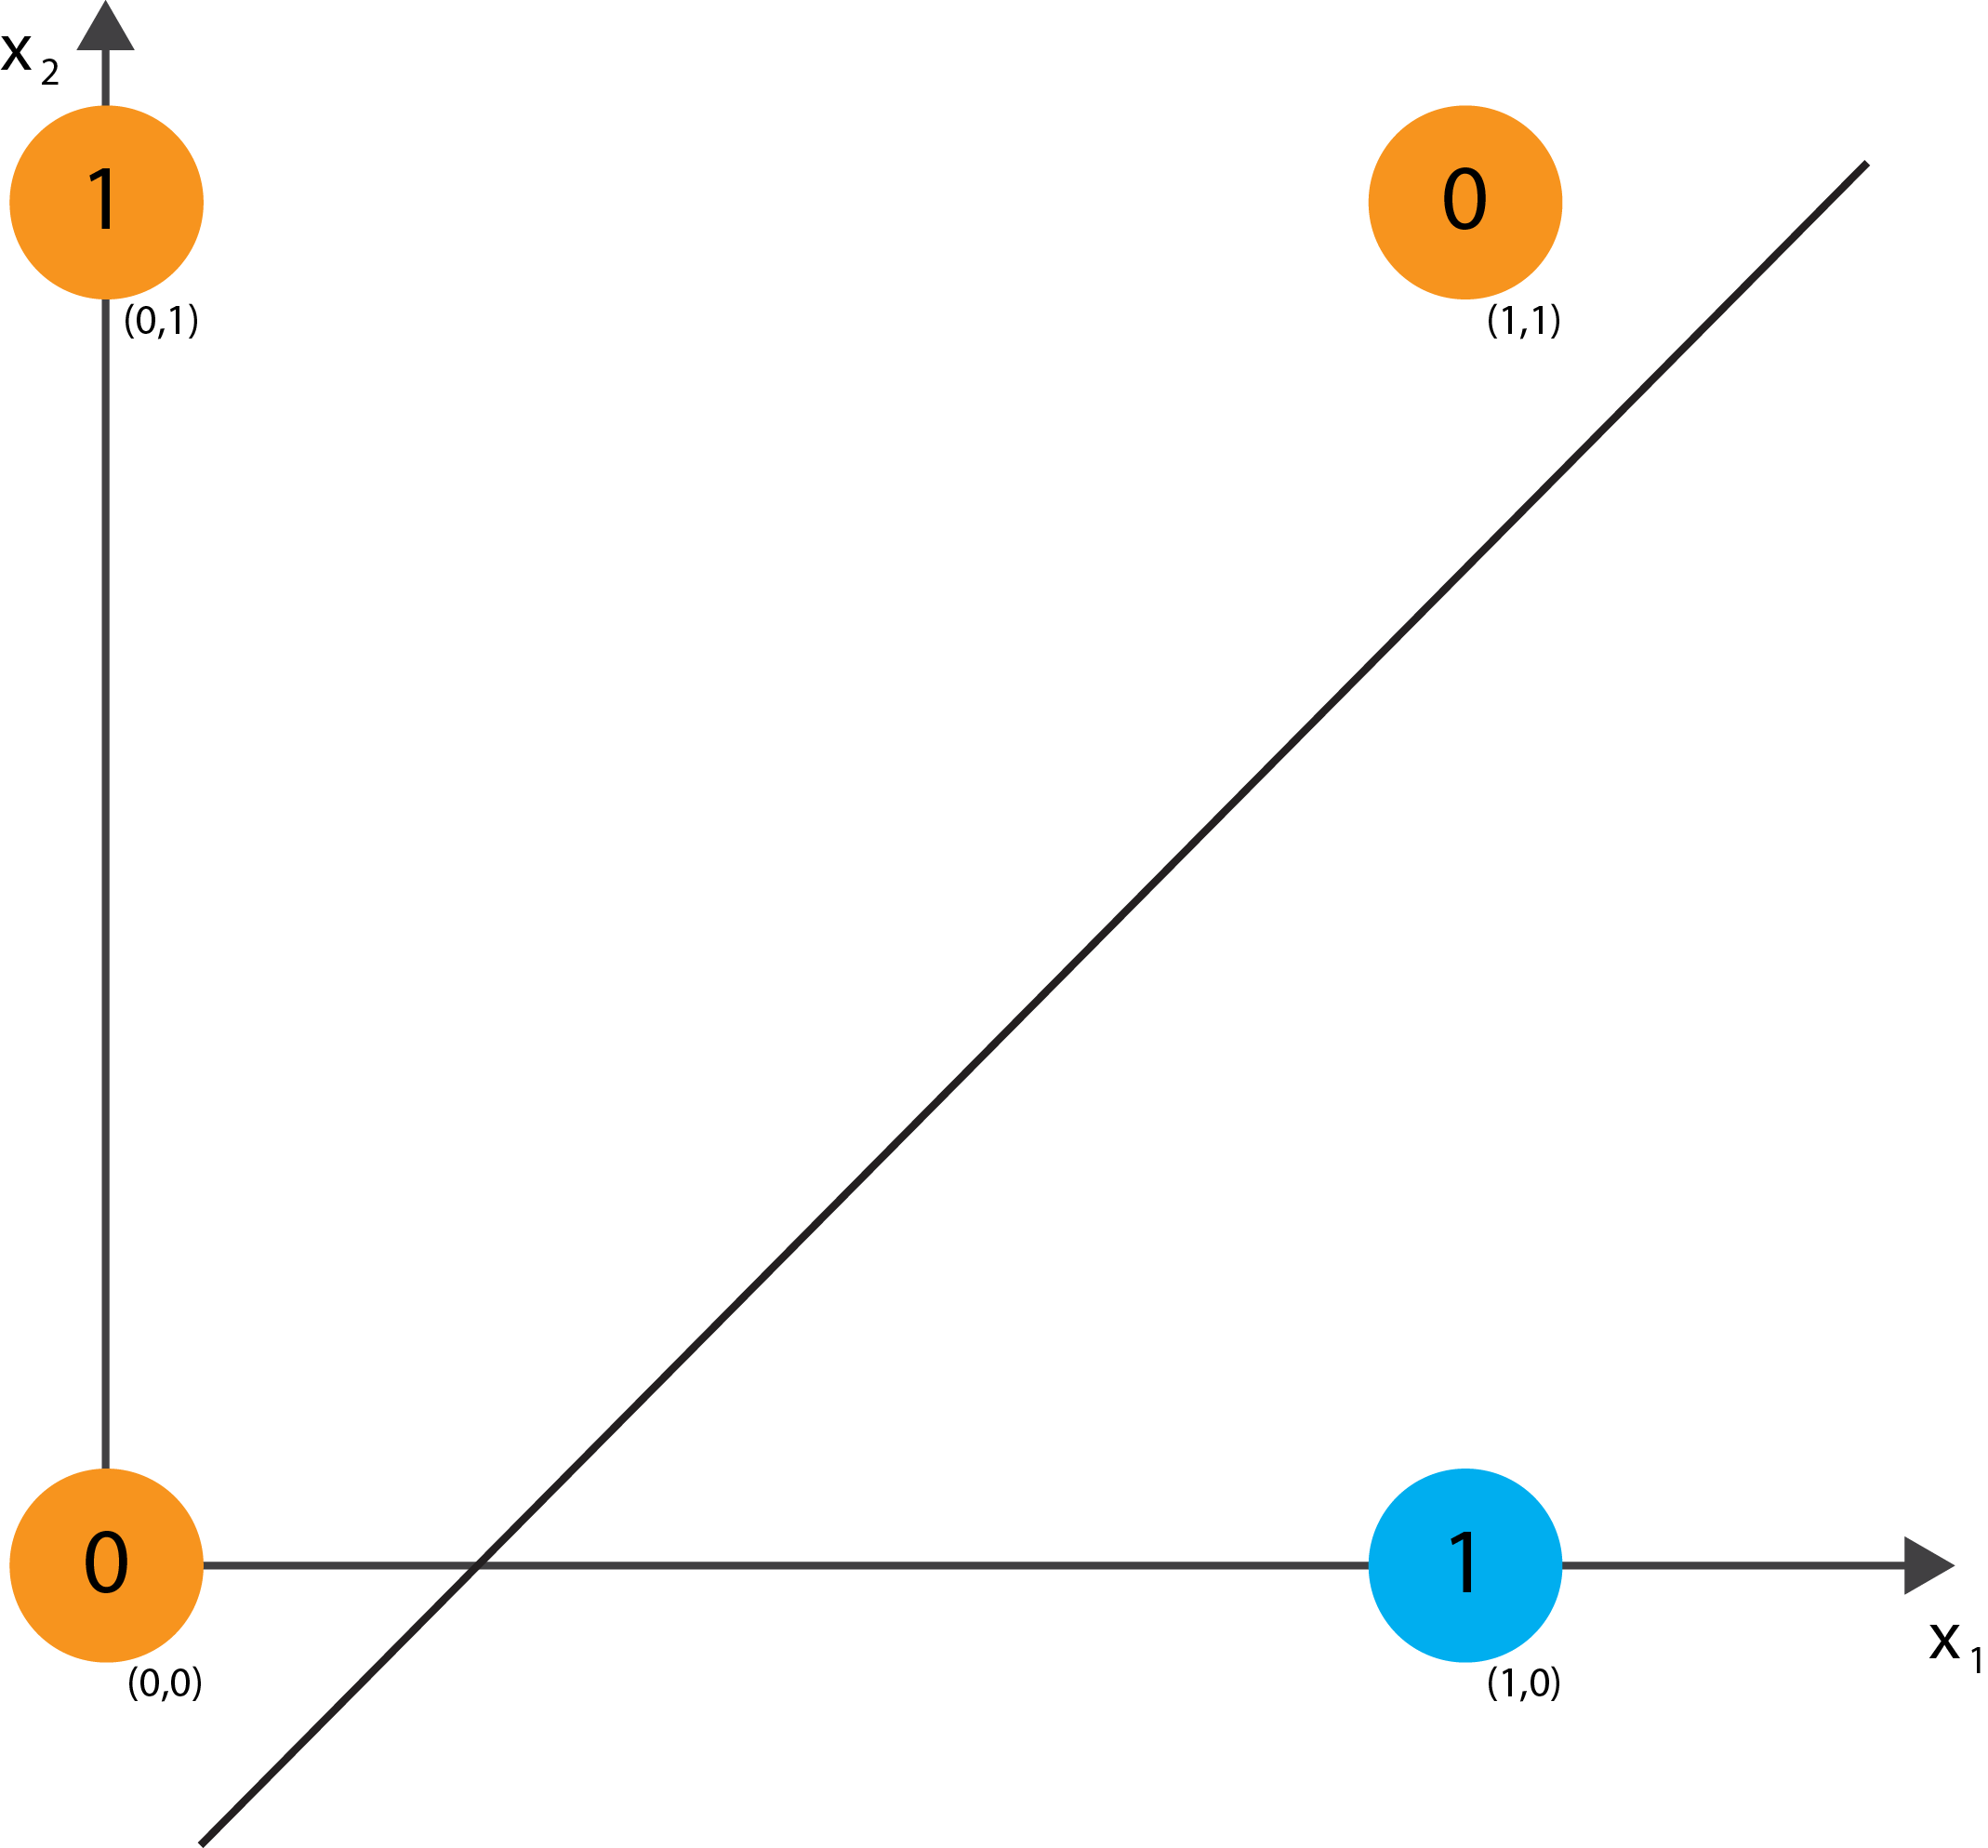
\includegraphics[width=0.22\textwidth]{svm/svm_xor.png}
    \caption{XOR nichtlinear separierbar in $\mathbb{R}^2$}
    \label{fig:perceptron_xor}
\end{figure}

Mit einem Trick, der Erhöhung der Dimension, können mehrlagige Perzeptronen auch nichtlinear separierbare Probleme lösen. 
So lässt sich bspw. das XOR-Problem in einem 3-dimensionalen Raum durch eine Hyperebene trennen (\ref{fig:perceptron_xor3d}).

\begin{figure}[htbp] \centering
    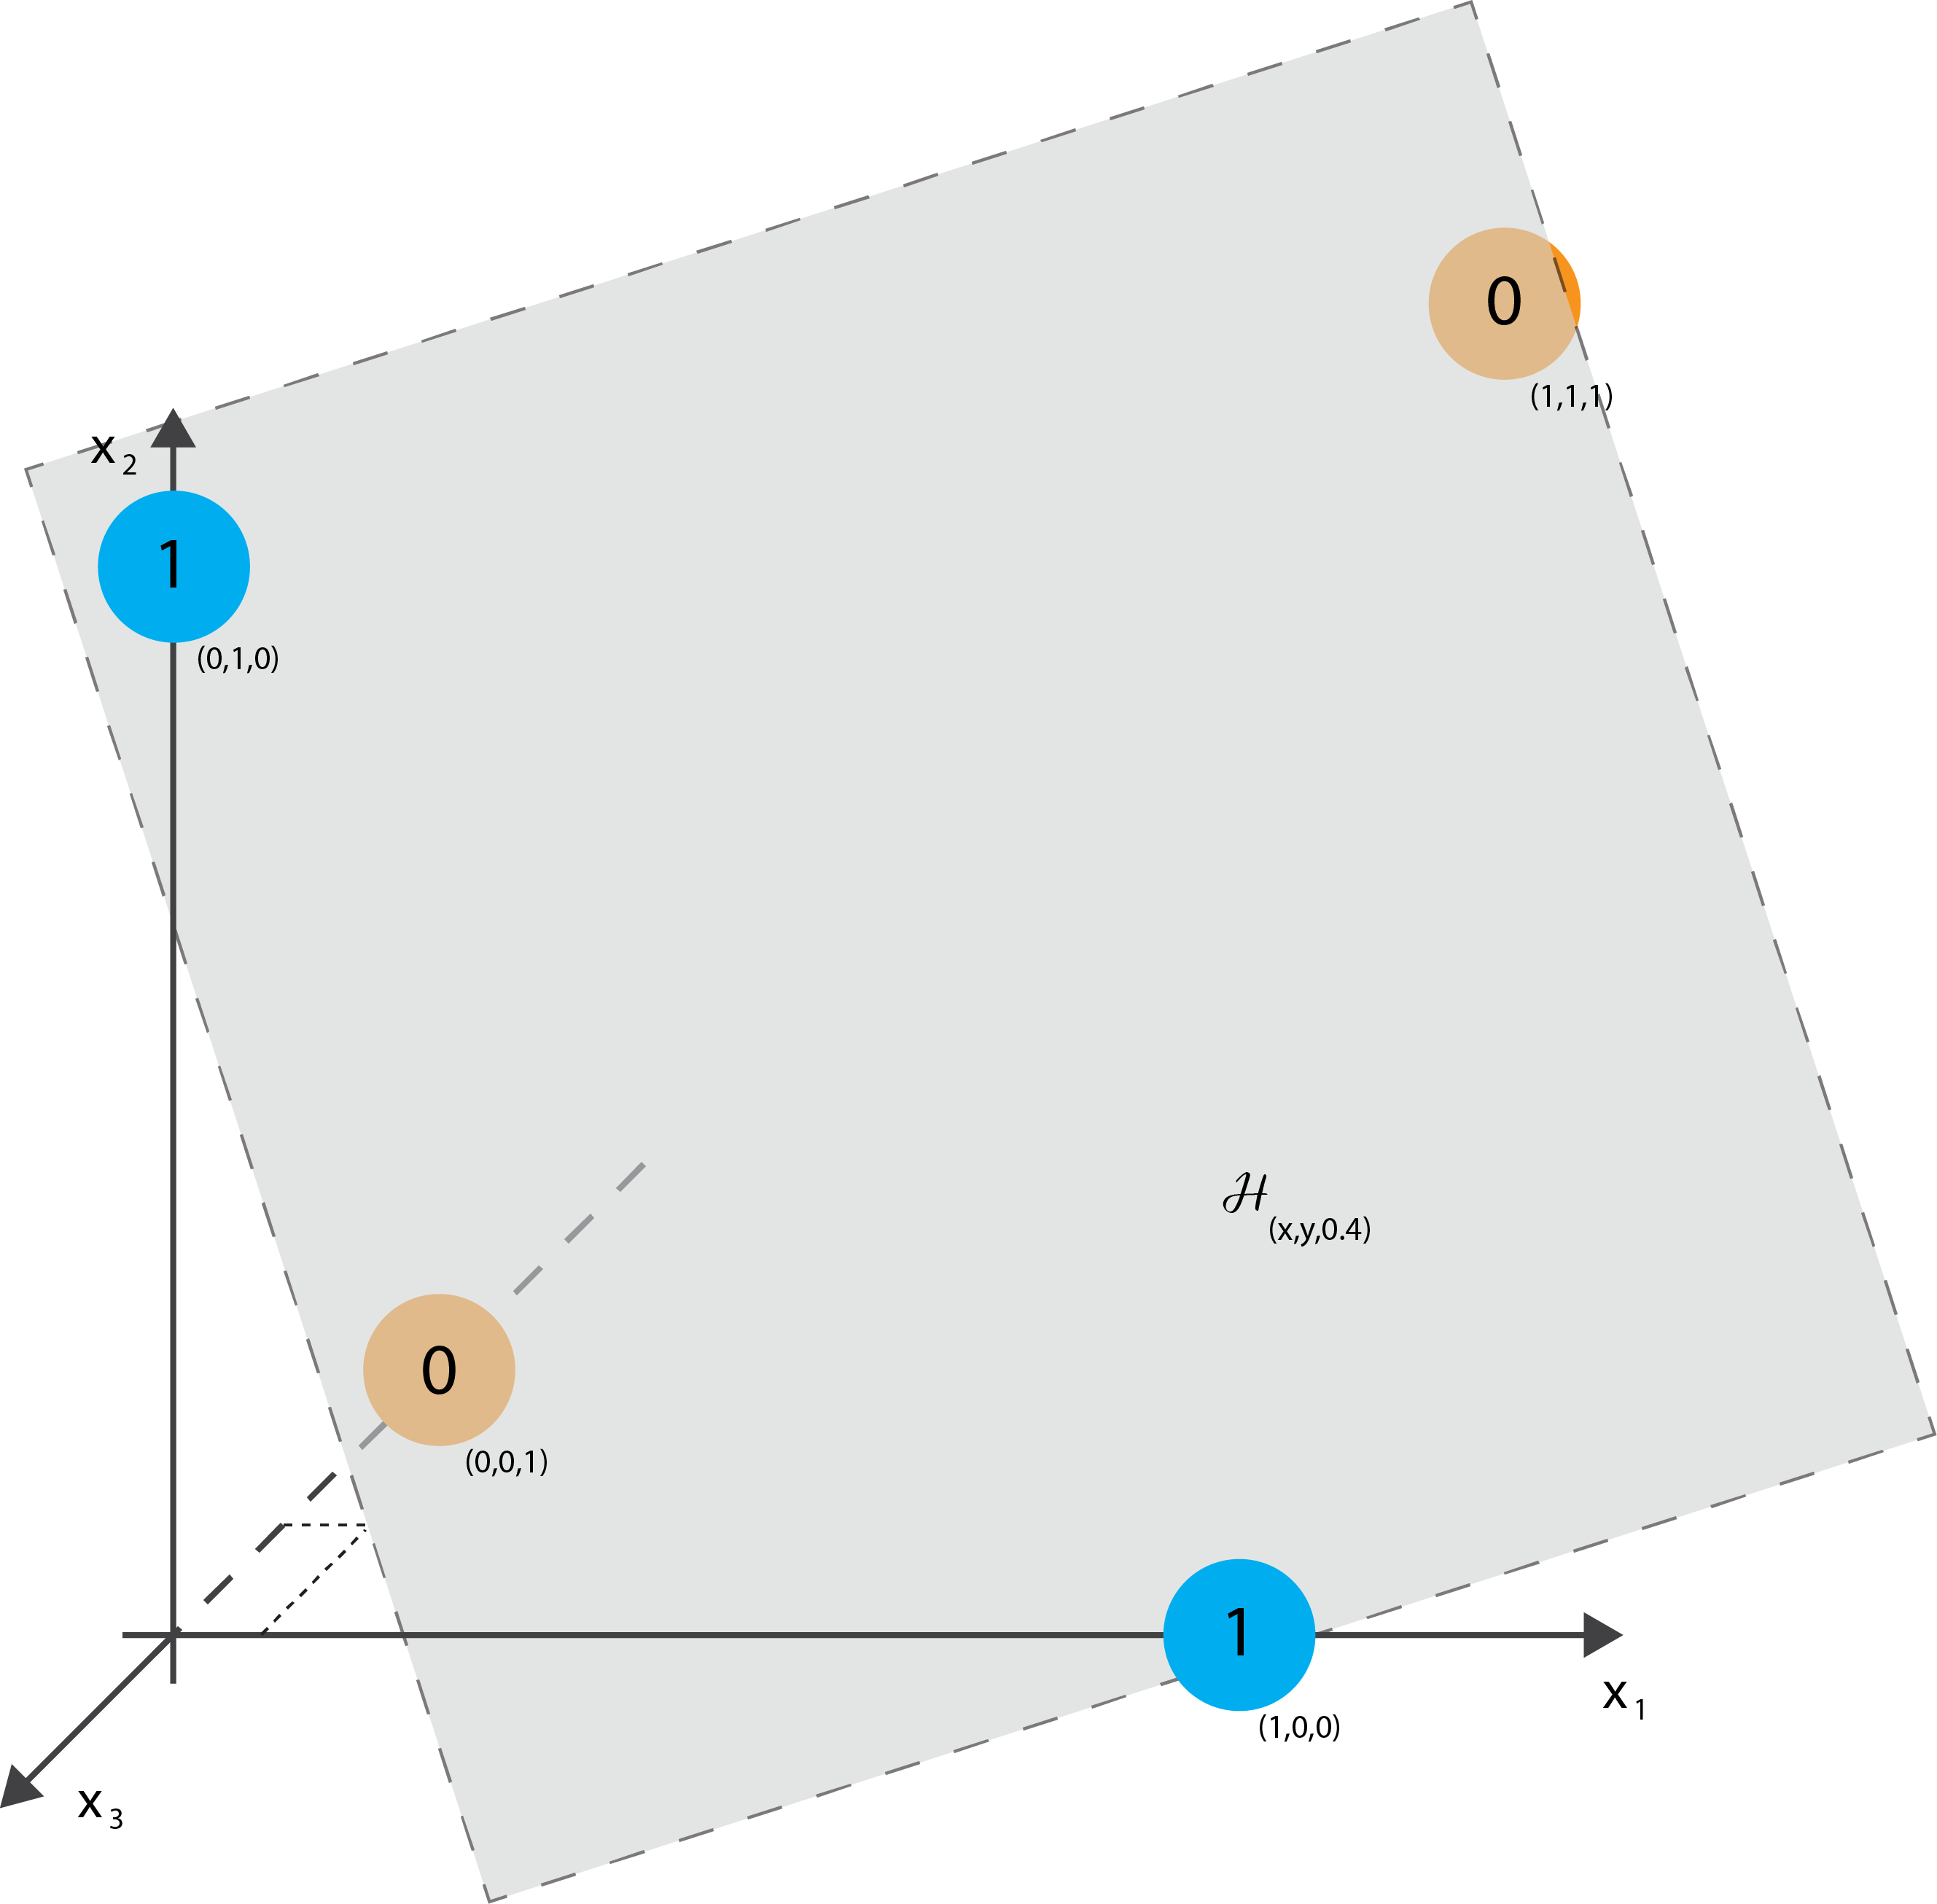
\includegraphics[width=0.22\textwidth]{svm/svm_xor_3d.png}
    \caption{XOR linear separierbar in $\mathbb{R}^3$}
    \label{fig:perceptron_xor3d}
\end{figure}

Die Wahl der richtigen Gewichte ist dabei nicht einfach, für komplexere Problemstellungen schier unmöglich. 
Um dennoch eine Problemlösung zu modellieren, die Eingaben richtig klassifiziert, gibt es einen Algorithmus, der die Gewichte automatisch anpasst.
Dieser Algorithmus setzt eine Trainingsmenge voraus, für dessen Eingabevektoren die zugehörigen Klassen bekannt sind. 
Durch Fehlerrückführung kann ein \ac{MLP} trainiert werden und das Netz kann die gewünschten Muster nach einer kontrollierten Trainingsphase klassifizieren.

Knapp 40 Jahre Jahre später veröffentlichte der sowjetisch-amerikanische Mathematiker Wladimir Wapnik \cite{Vapnik} das Prinzip der Support-Vector-Machines (\ac{SVM}).

Im Gegensatz zu \ac{MLP}s wird die Anpassung der Trennung nicht empirisch durch Trainingsmethoden, sondern durch die Datengrundlage mathematisch optimal ermittelt. 
SVMs können auch nichtlinear separierbare Probleme lösen, ohne die Dimension der Eingabe zu erhöhen. 
Die Hauptidee dabei ist die Repräsentation der Daten zu verändern. 
Mit Hilfe des sogenannten Kernel-Tricks werden die Daten in einen höherdimensionalen Raum transformiert. 

Support Vector Machines erfreuen sich großer Beliebtheit, da sie in der Regel wesentlich performanter vernünftige Vorhersagen treffen können. Lediglich durch die Lokalisierung des Objekts im Koordinatensystem wird klassifiziert. Dadurch, dass eine trainierte SVM eine Trenngerade generiert, kann durch einfache Hilfsmittel aus der linearen Algebra die relative Position bestimmt werden. Es wird also entschieden, ob das zu klassifizierende Objekt "{}oberhalb"{} oder "{}unterhalb"{} der Trenngeraden liegt. Allerdings ist zu beachten, dass für sehr große Datenmengen die \ac{SVM} eine sehr lange Trainingsphase benötigt, da der Algorithmus die Inversion der Eingabematrix benutzt. Das Bilden der inversen Matrix hat eine Laufzeit zwischen $\mathcal O(n^2)$ und $\mathcal O(n^3)$ und ist damit sehr aufwändig.

\subsection{Funktionsweise der SVM}

\subsubsection{Optimale Trennung}
Mit einem Satz von Merkmalsvektoren (Merkmalsraum) und dessen Klassenzugehörigkeiten $\{ (x_1, y_1), ..., (x_m, y_m) | x_i \in \mathcal{X}, y_i \in \{-1, 1\}, m \in \mathbb{N} \}$ wird eine mathematische Gerade errechnet,
die in einem Koordinatensystem betrachtet die Daten räumlich in zwei Klassen trennt. 

Die Gerade (Hyperebene im mehrdimensionalen Raum) trennt die Merkmalsräume bestmöglich und dient als Entscheidungsfunktion für die Klassifikation. Sie ist gegeben durch den Normalenvektor $w$ und den sogenannten Bias $b$, dem Abstand der Ebene zum Ursprung. Diese Form erweist sich als besonders praktisch, da durch Einsetzen von $x$ der direkte Abstand zur Hyperbene resultiert.
Intuitiv ist klar, dass alle Punkte auf der Hyperebene selbst keinen Abstand haben, die Formel der Hyperebene (\ref{eq:svm_hyperplane}) lautet demnach: 
 
\begin{equation}
\label{eq:svm_hyperplane}
    \mathcal{H}: \{ x \,|\, \langle w,x \rangle + b = 0 \}
\end{equation}
 
Allein durch das Vorzeichen der Entscheidungsfunktion ordnet die \ac{SVM} die Eingabe einr Klasse zu. Dabei können nur zwei Klassen  prognostiziert werden. Die Klasse gehört demnach entweder zur Klassenmenge \ref{eq:svm_decision0} oder zu \ref{eq:svm_decision1}.

\begin{eqnarray}
    \mathcal{C}_{-1}: \{ c \,|\, \operatorname{sgn}(\langle w,x \rangle + b) = -1 \} \label{eq:svm_decision0} \\
    \mathcal{C}_1: \{ c \,|\, \operatorname{sgn}(\langle w,x \rangle + b) = 1 \} \label{eq:svm_decision1}
\end{eqnarray}

Die nächstliegenden Vektoren zur Trenngeraden werden als Stützvektoren, der Abstand als Margin $M$ bezeichnet (Abb. \ref{fig:svm_separator}). 

\begin{figure}[htbp] \centering
    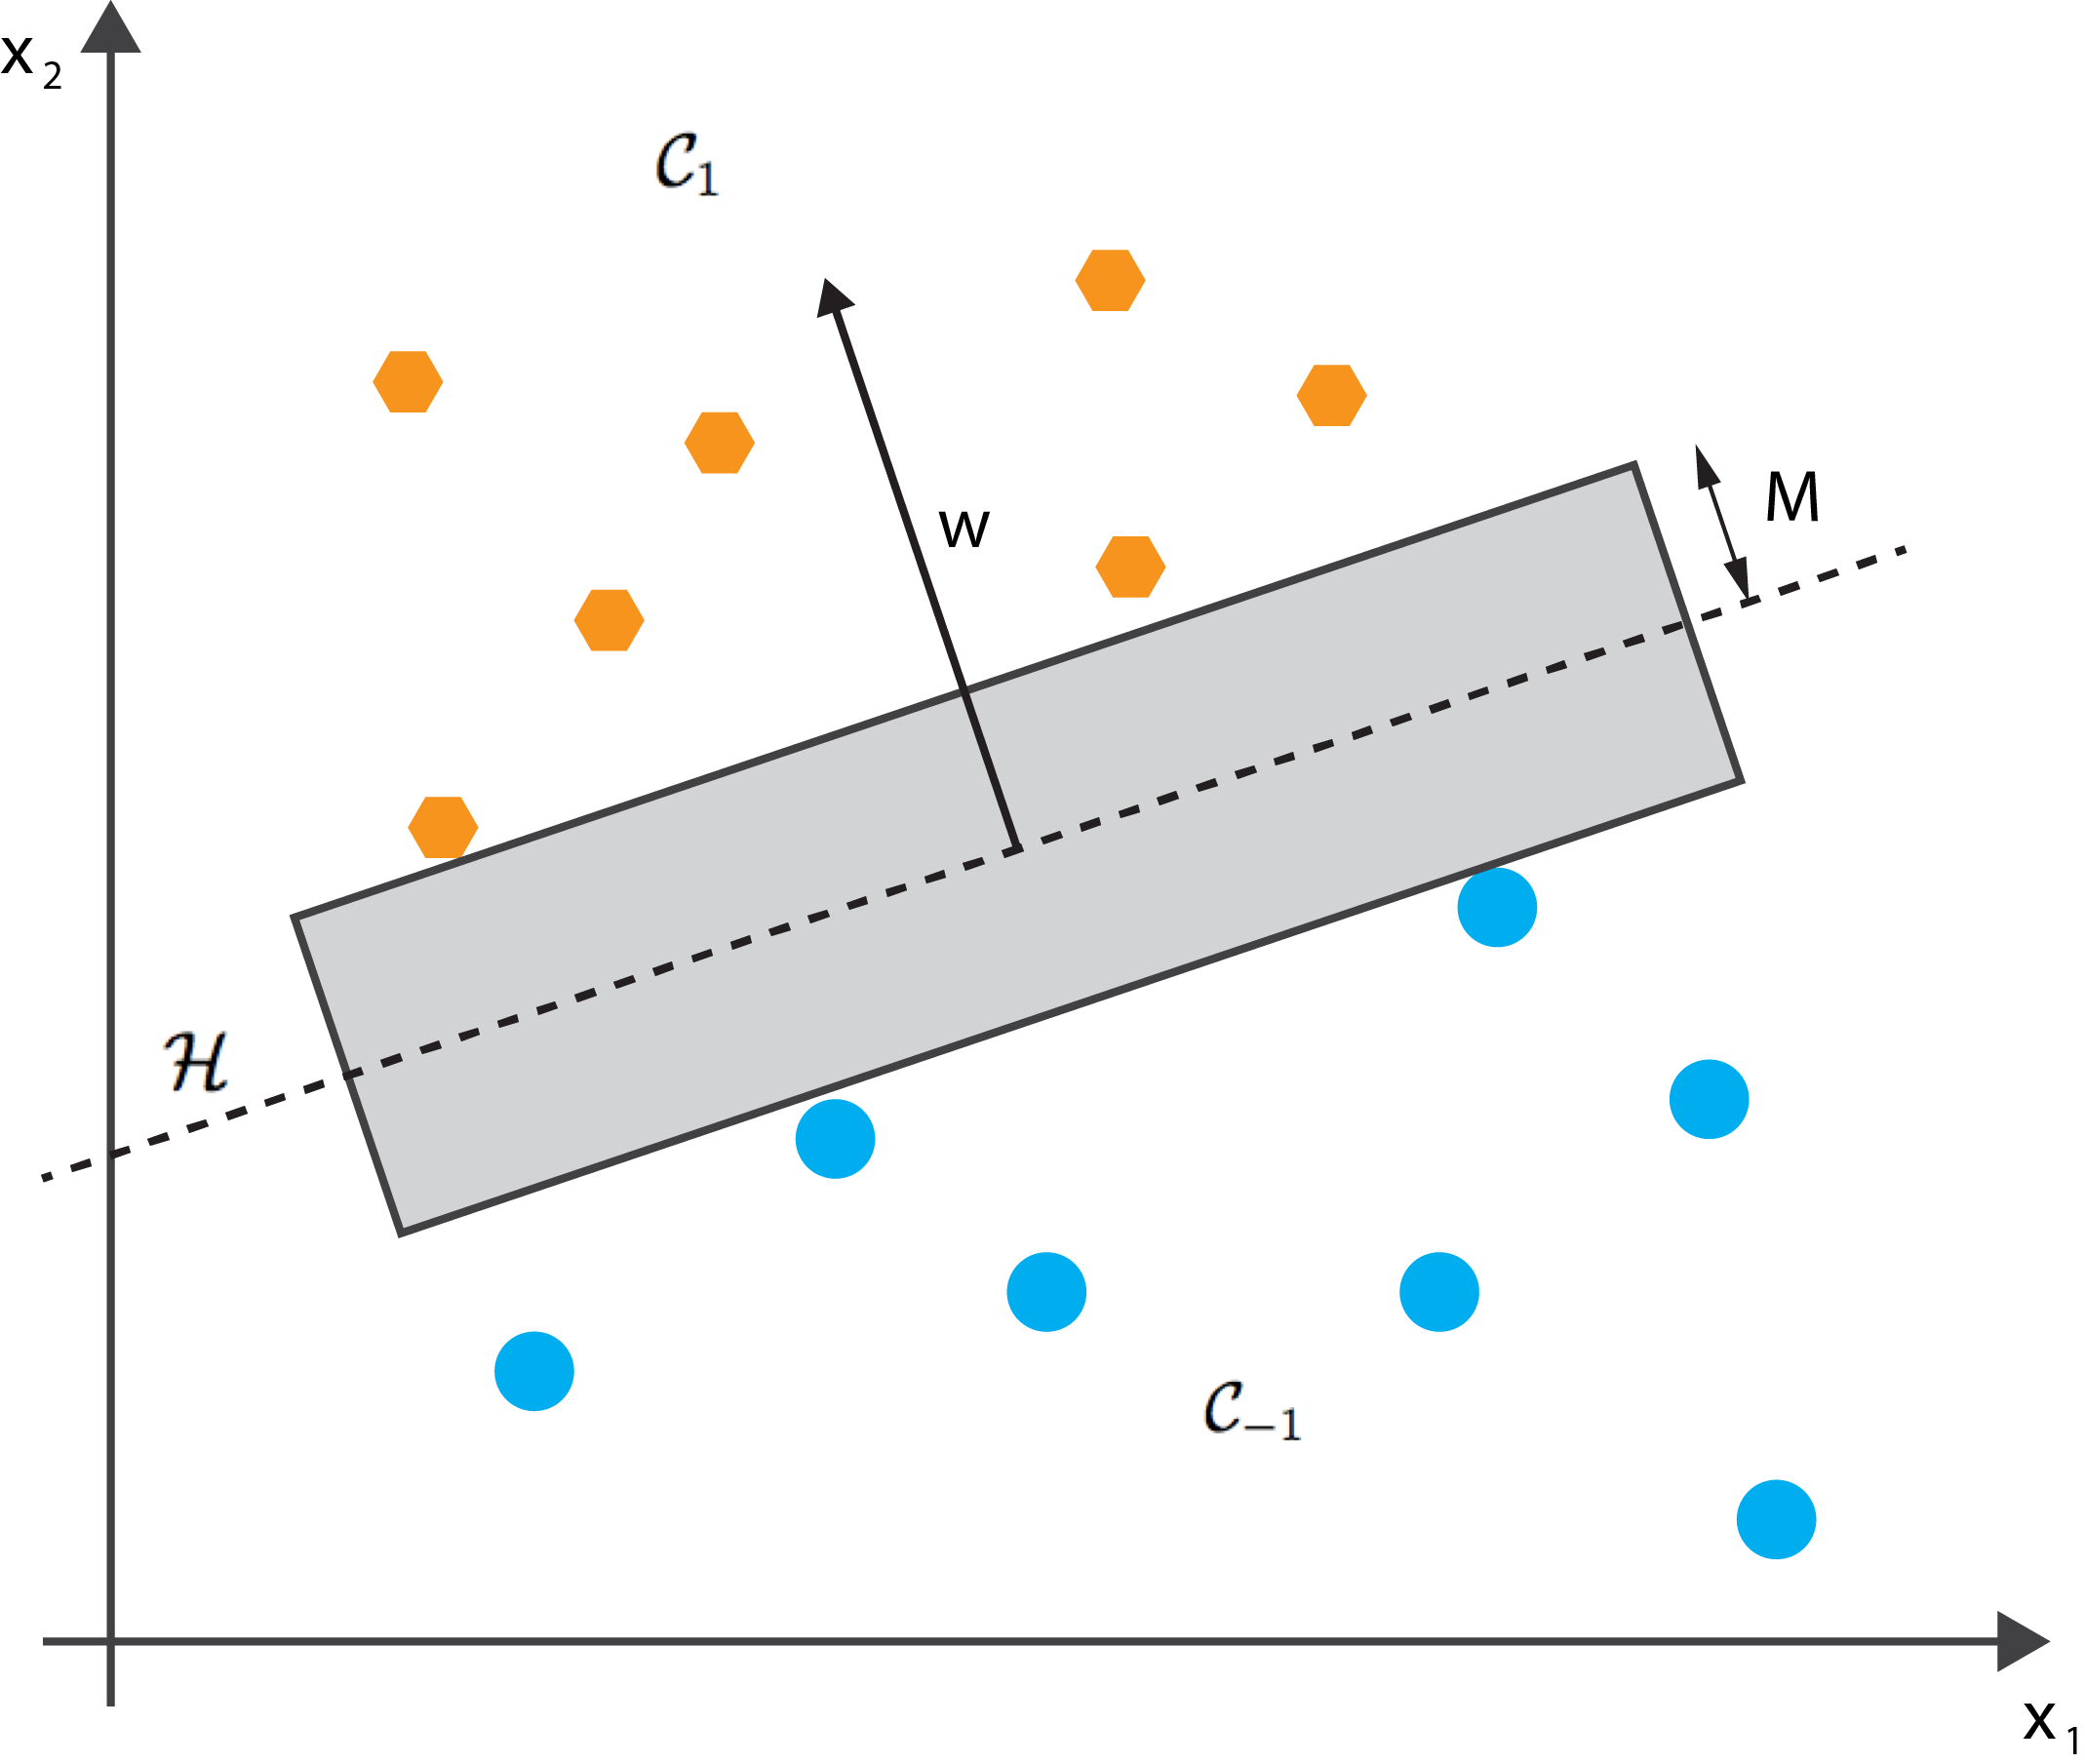
\includegraphics[width=0.43\textwidth]{svm/svm_overview.png}
    \caption{Trenngerade einer SVM}
    \label{fig:svm_separator}
\end{figure}

Die Stützvektoren bilden das tragende Konstrukt der Entscheidungsfunktion. 
Alle andere Merkmalsvektoren haben keinen Einfluss auf die Trennung, was die Namensgebung der Stützvektoren begründet. 
Das macht die \ac{SVM} zu einem sehr transparenten und performanten Klassifikator. 

\subsubsection{Kernel-Trick}
Es ergeben sich Unregelmäßigkeiten bei der Lösung von nichtlinear separierbaren Problemen und der Klassifikation von mehr als 2 Klassen.
Im Gegensatz zu den MLPs umgeht man diesen Umstand nicht mit der Erhöhung der Dimension. 
Die \ac{SVM}s setzen in diesem Falle auf die Transformation der Datenrepräsentation. 

\begin{figure}[htbp] \centering
    \subfigure[$x$ nichtlinear separierbar in $\mathbb{R}^n$]{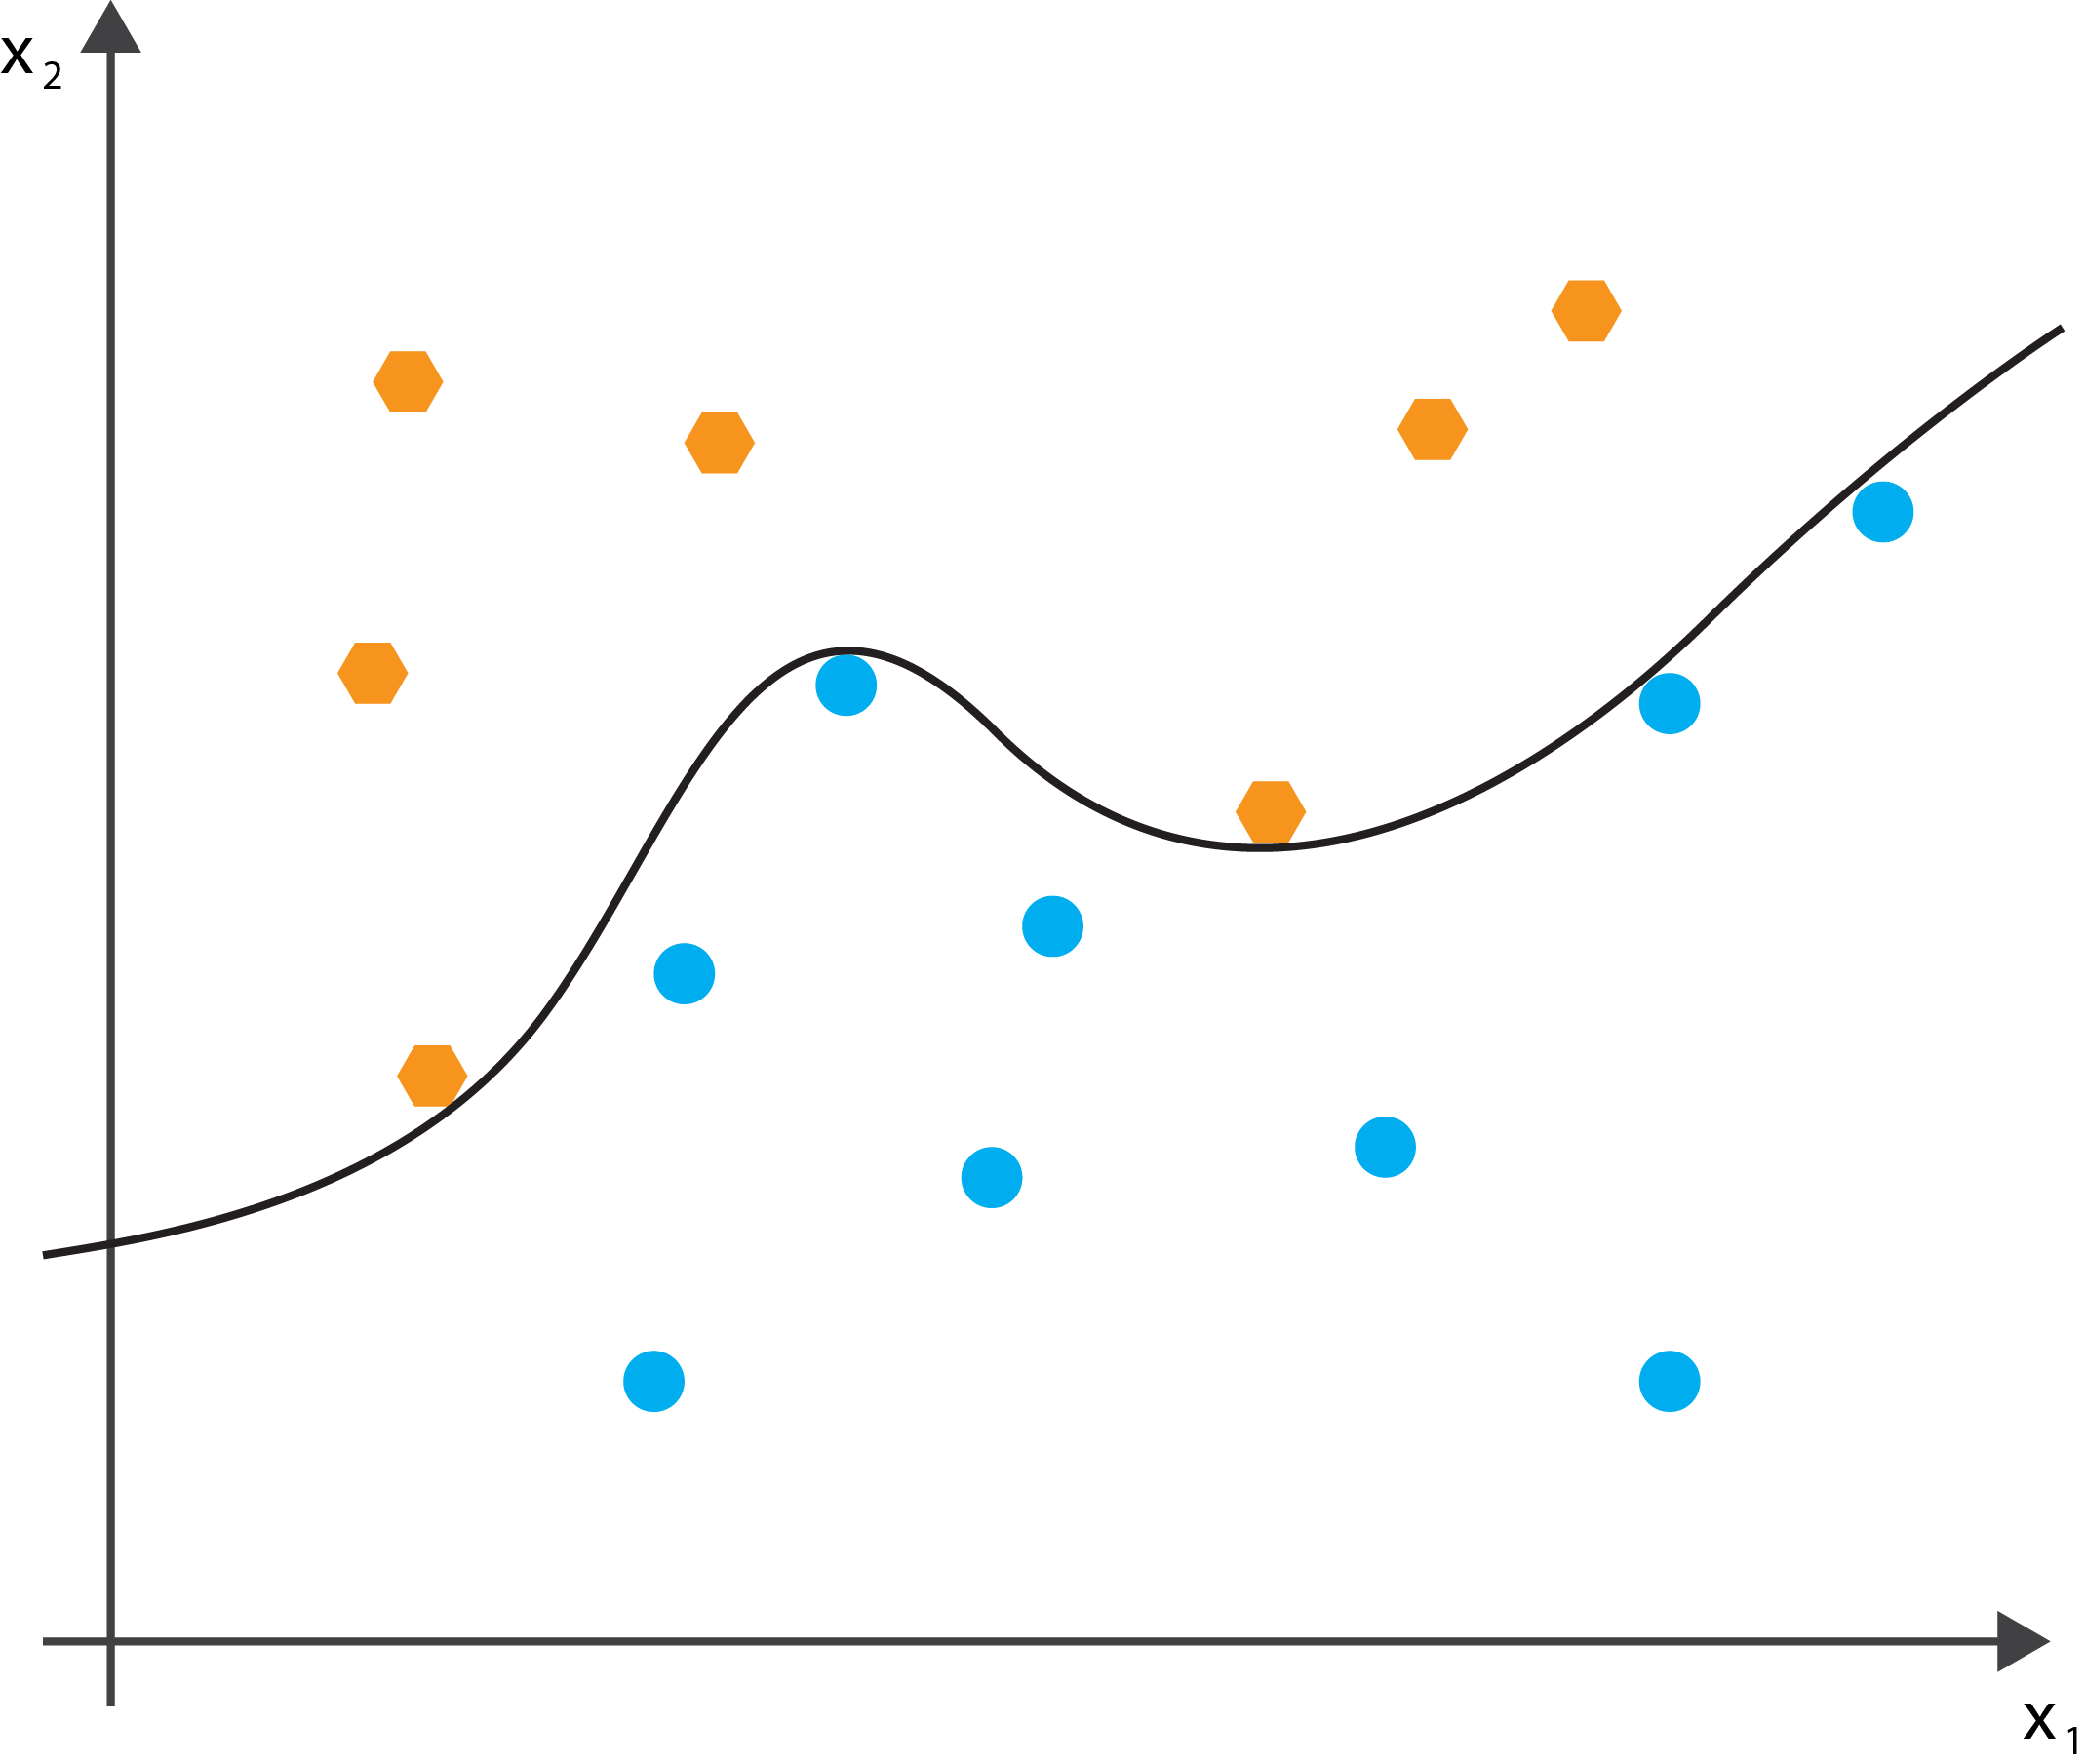
\includegraphics[width=0.22\textwidth]{svm/svm_fitting-line.png}}
    \subfigure[$\phi(x)$ linear separierbar in $\mathbb{R}^h, h>n$]{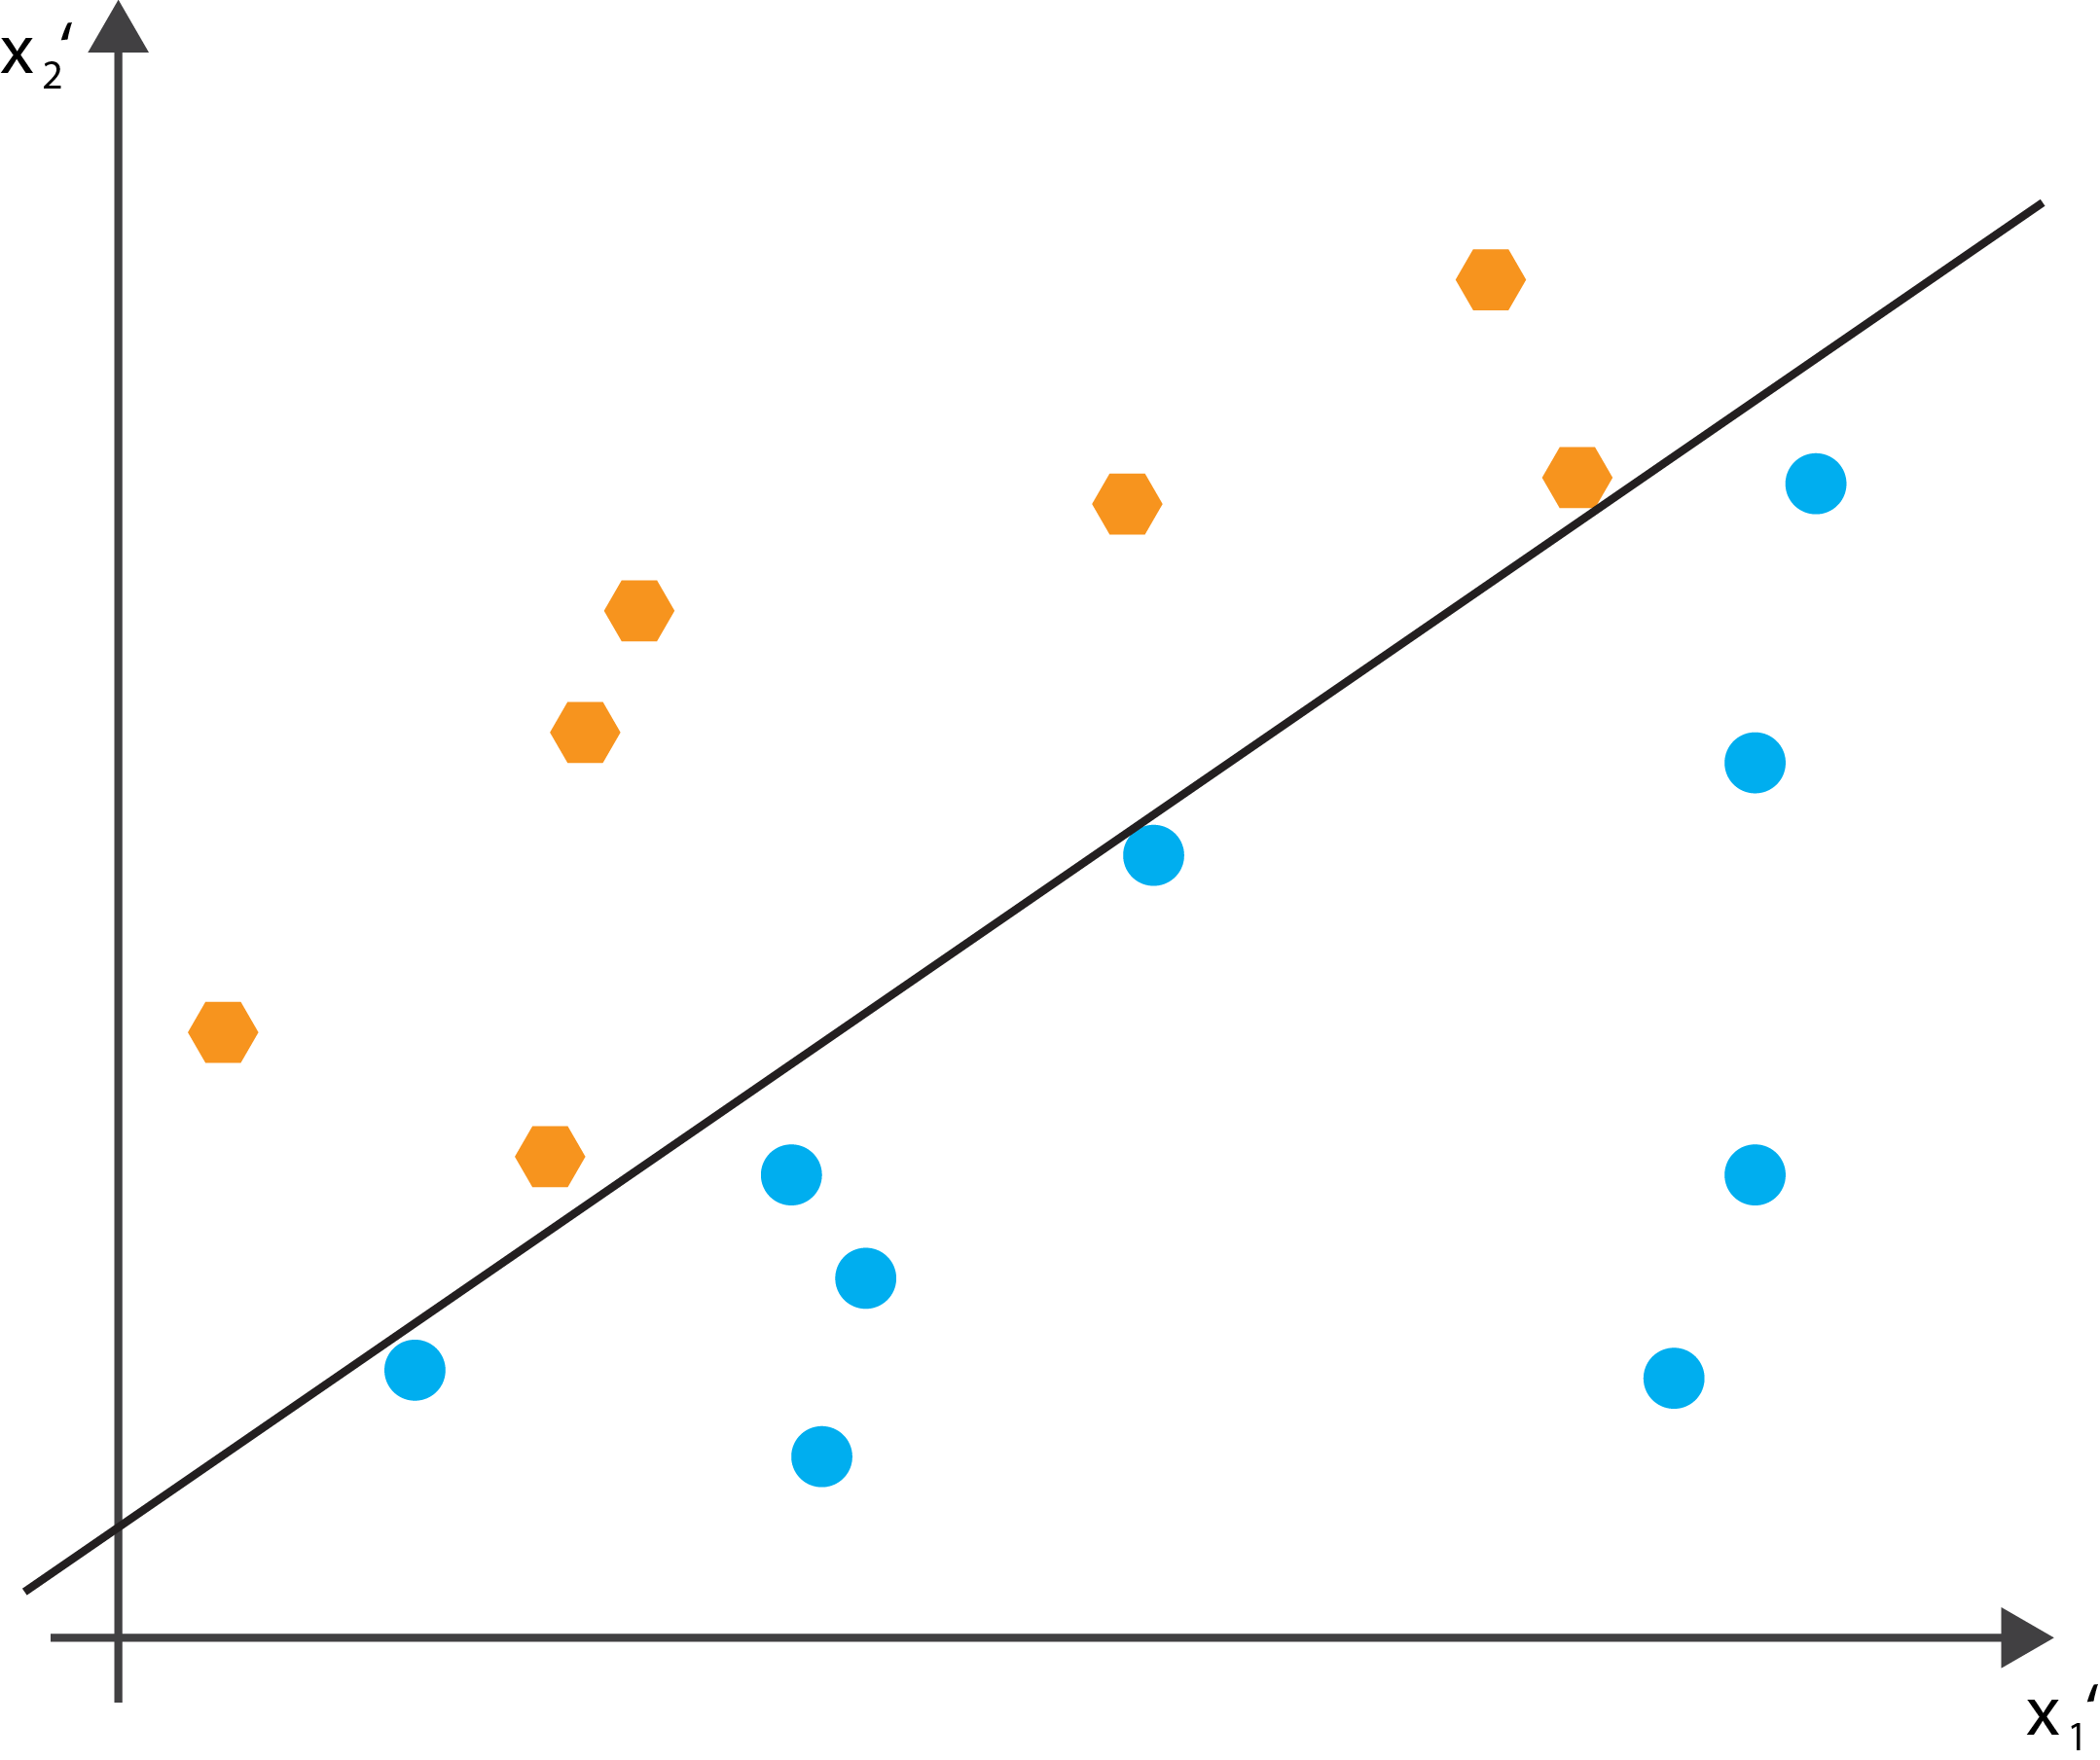
\includegraphics[width=0.22\textwidth]{svm/svm_linear-fitting.png}}
    \caption{Kernfunktion $\phi$}
    \label{fig:svm_kernel}
\end{figure}

Mit Hilfe von Kernfunktionen (\ref{eq:svm_kernel_function}) lassen sich Daten von $\mathbb{R}^n$ in einen höherdimensionalen Raum $\mathbb{R}^h$ transformieren, in dem sie linear separierbar erscheinen (Abb. \ref{fig:svm_kernel}).

\begin{equation}
\label{eq:svm_kernel_function}
\begin{split}
    \phi : & \mathbb{R}^n \to \mathbb{R}^h \\
    & x \mapsto \phi(x)
\end{split}
\end{equation}

Als Bedingung des Raums $\mathbb{R}^h$ gilt, dass das Skalarprodukt erklärt ist.
Wir haben nach der Transformation also die neue Form (\ref{eq:svm_kern_tranformation}).
In der müssen wir nun das Skalarprodukt $\langle\phi(w),\phi(x)\rangle$ ausrechnen, was sehr schwierig (bzw. unmöglich) ist, wenn die Dimension von $\mathbb{R}^h$ zu groß wird.

\begin{equation}
\label{eq:svm_kern_tranformation}
    \mathcal{C}: \{ c_i \,|\, \operatorname{sgn}(\langle \phi(w),\phi(x) \rangle + b) = i \}
\end{equation}

Dadurch, dass die Trainingspunkte $x$ nur in Skalarprodukten auftauchen, können wir uns des Kernel-Tricks bedienen.
Kernfunktionen, die in $\mathbb{R}^n$ leben, zeichnen sich durch eine spezielle Eigenschaft aus, da sie sich verhalten wie ein Skalarprodukt in $\mathbb{R}^h$ (\ref{eq:svm_kern_trick}).

\begin{equation}
\label{eq:svm_kern_trick}
    \mathcal{K}(w,x) = \langle\phi(w),\phi(x)\rangle
\end{equation}

Es kann also das Skalarprodukt $\langle\phi(w),\phi(x)\rangle$ in $\mathbb{R}^h$ ausgerechnet werden, ohne die Daten mittles $\phi$ zu transformieren. 
Das Beispiel \ref{fig:ex_kernel} verdeutlicht die Anwendung des Kernel-Tricks  anhand einer polynomiellen Kernfunktion.

\renewcommand{\figurename}{Bsp.}
\begin{figure}[htbp]
\begin{equation*}
\label{eq:svm_kernel_example}
\begin{split}
    \text{Seien } w,x & \in \mathbb{R}^2 \text{ und}\\
    \phi : & \mathbb{R}^2 \to \mathbb{R}^3\\
    & \begin{pmatrix}
    x_1 \\
    x_2
    \end{pmatrix}
    \mapsto
    \begin{pmatrix}
    x_1^2 \\
    \sqrt{x_1x_2} \\
    x_2^2
    \end{pmatrix}\\
    \text{dann ist:} &\\
    \langle \phi(w),\phi(x) \rangle = & \:\langle \begin{pmatrix}
    w_1^2 \\
    \sqrt{w_1w_2} \\
    w_2^2
    \end{pmatrix},
    \begin{pmatrix}
    x_1^2 \\
    \sqrt{x_1x_2} \\
    x_2^2
    \end{pmatrix} \rangle \\
    \\
    = & \:w_1^2x_1^2 + 2 w_1x_1w_2x_2 + w_2^2x_2^2 \\
    = & \:(w_1x_1 + w_2x_2)^2 \\
    = & \:\langle w,x \rangle^2 \overset{\text{(def)}}= \mathcal{K}(w,x)
\end{split}
\end{equation*}
    \caption{Beispiel einer polynomiellen Kernfunktion}
    \label{fig:ex_kernel}
\end{figure}

Nicht jede beliebige Funktion ist eine Kernfunktion. Kernfunktionen müssen die Bedingungen nach dem Satz von Mercer \cite[S. 127]{Marsland} erfüllen. 
Gängige Kernfunktionen sind:

\begin{itemize}
\item{linear: $\mathcal{K}(w,x) = \langle w,x \rangle$}
\item{polynomiell: $\mathcal{K}(w,x) = (\gamma\langle w,x \rangle+c_0)^d$}
\item{sigmoid: $\mathcal{K}(w,x) = \tanh(\gamma\langle w,x \rangle+c_0)$}
\item{rbf: $\mathcal{K}(w,x) = \exp(- \gamma \|w - x \| ^2)$}
\end{itemize}

\subsubsection{Klassifikation von mehreren Klassen}
Da die \ac{SVM} als binärer Klassifikator entwickelt wurde, müssen für eine Klassifikation von mehr als zwei Klassen Strategien entwickelt werden, um das Prinzip der \ac{SVM} zu erweitern. 
Ein Verfahren ist die \textit{Einer gegen den Rest}-Klassifikation. 
Bei dieser Technik wird für jedes zu klassifizierende Objekt eine binäre \ac{SVM}-Instanz trainiert. 
Für jede \ac{SVM} wird eine Klasse separiert, die anderen Klassen werden nicht unterschieden und als negative Beispiele zu einer Restklasse definiert. 
Die Vorraussage eines Objektes ergibt sich aus der Auswertung aller \ac{SVM}-Instanzen. 
Es ist nun möglich, dass mehrere Instanzen eine positive Klassenzuordnung feststellen und nicht die Restklasse klassifizieren. 
In diesem Fall entscheidet sich das \textit{Einer gegen den Rest}-Verfahren für die Klasse, dessen \ac{SVM} die höchste Ausgabe erzeugt (\textit{winner-takes-all}). 
Als höchstes Ergebnis wird der größte Abstand zur Trennhyperebene angenommen. 
Offensichtlich erhöht sich die Laufzeit der Trainingsphase mit der Anzahl der Klassen $|\mathcal{C}|$. 
Glücklicherweise beeinflusst das nicht die Laufzeitanalyse in der $\mathcal{O}$-Notation (\ref{eq:svm_winner_runtime}). 

\begin{equation}
\label{eq:svm_winner_runtime}
    \underbrace{\mathcal{O}(n) + ... + \mathcal{O}(n)}_{|\mathcal{C}|-mal} = |\mathcal{C}| \cdot \mathcal{O}(n) = \mathcal{O}(n)
\end{equation}

Sind die SVMs trainiert, beeindrucken sie durch rasante Klassifikation. 
Dies ermöglicht uns eine echtzeitnahe Gestenerkennung.

%%%%%%%%%%%%%%%%%%%%%%%%%%%%%%
%%%%%%%%%%%%%%%%%%%%%%%%%%%%%%
%%%%%%%%%%%%%%%%%%%%%%%%%%%%%%

\subsection{Anwendung auf das Projekt}
Zur Klassifikation der Gesten wird eine \ac{SVM} benutzt, die mit geringfügig angepassten und von den Standards des verwendeten Python-Moduls abweichenden Werten der entsprechenden Parameter trainiert wird. 
Für das Training erwartet die \ac{SVM} neben einem Eingabevektor mit 320 Werten noch die dazugehörige Klasse.
Während der Live-Klassifikation von Gesten, beziehungsweise deren Eingabevektoren, wird die trainierte \ac{SVM} für die Erkennung verwendet.
Die Eingabevektoren müssen dabei in ihrer Dimension den Trainingsdaten entsprechen.

Der nächste Abschnitt widmet sich der Datenaufbereitung, insbesondere der Reduzierung der Dimension eines Eingabevektors und der entsprechenden Vorverarbeitung.
\begin{figure*}[htbp] \centering
    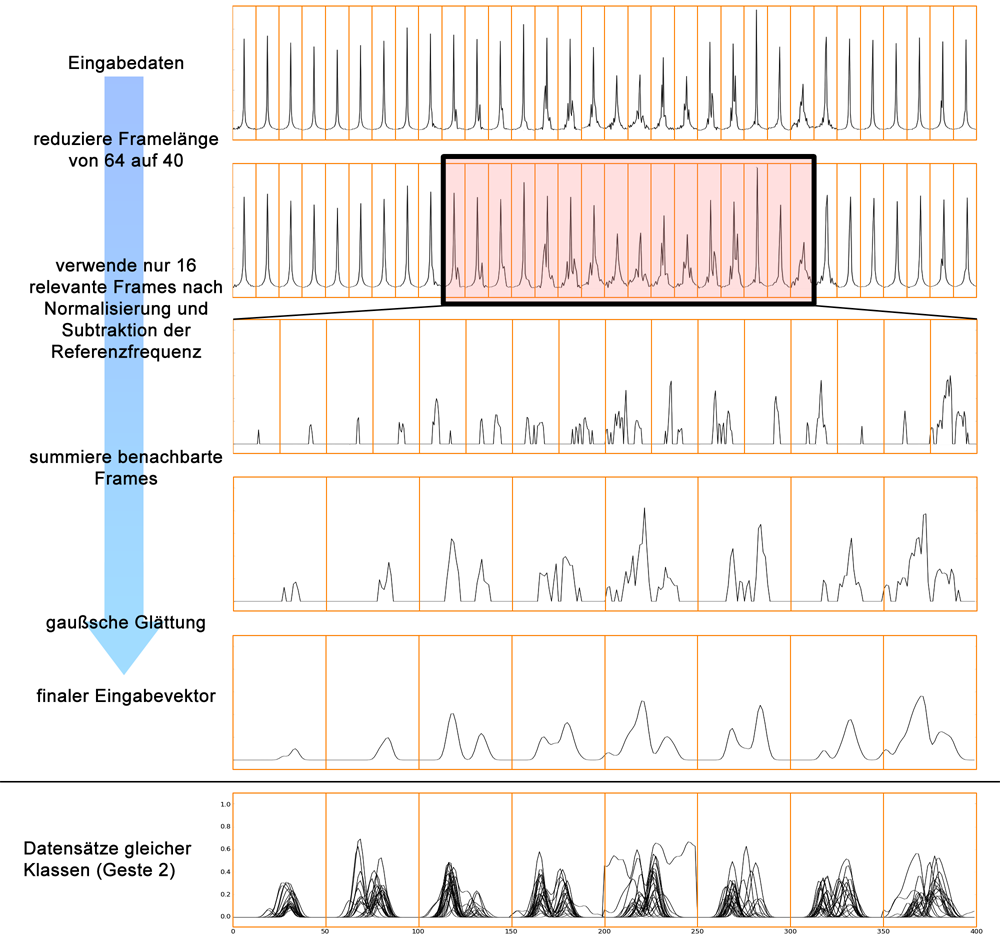
\includegraphics[width=0.65\textwidth]{svm/svm_preprocessing_steps.png}
    \caption{Datenaufbereitungsschritte}
    \label{fig:svm_preprocessing_steps}
\end{figure*}

\subsubsection{Datenaufbereitung}\label{sec:svm_data} 
In \autoref{sec:intro} wurde die Aufnahme und die generelle Vorverarbeitung der Daten bereits erläutert, bevor diese an die entsprechenden Klassifikatoren weitergeleitet werden.
Da jeder Klassifikator aufgrund seiner Funktionsweise unterschiedlich mit den Eingabedaten arbeitet, ist eine entsprechende und auf den jeweiligen Klassifikator angepasste Datenaufbereitung notwendig.
Gleichzeitig kann durch eine entsprechende Vorverarbeitung gegenüber unverarbeiteten Daten das Problem der Klassifikation von unterschiedlichen Datensätzen verallgemeinert und somit die Trainingszeit verringert werden.
Dieser Abschnitt befasst sich mit der spezifischen Datenaufbereitung für den \ac{SVM}-Klassifikator. 
Eine entsprechende grafische Visualisierung aller Datenaufbereitungsschritte befindet sich in \autoref{fig:svm_preprocessing_steps}.
\paragraph{Eingabevektordimensionsreduzierung}\label{sec:svm_reduce}$\;$ \\
Bei der Betrachtung der Trainingsdaten, die jeweils aus insgesamt 32 Frames zu je 64 Werten bestehen, wird offensichtlich, dass die durch den Doppler-Effekt verursachten Frequenzverschiebungen in einem begrenzten Umfeld der Referenzfrequenz von $18\text{,}5\text{ kHz}$ herum sattfinden.
Zudem stellt sich heraus, dass nur ein Bruchteil der ursprünglich veranschlagten 32 Frames pro Geste relevante Informationen enthält, da die Ausführung einer Geste meist zwischen 8 und 20 Frames dauert und nur innerhalb dieser Frame-Anzahl Frequenzverschiebungen verursacht.
Aufgrund dieser beiden Gründe werden im ersten Schritt der Reduzierung der verwendete Wertebereich eines Frames von 64 auf 40 verkleinert und im nächsten Reduzierungsschritt sowohl für das Training der \ac{SVM} als auch für die Live-Klassifikation nur 16 Frames pro Geste verwendet. 

Die dritte Reduzierung wird mittels der Addition benachbarter Frames erzielt, so dass letztlich nur noch jeweils 8 Frames zu je 40 Werten pro Datensatz/Geste existieren.
Im Anschluss erfolgt die Transformation in ein eindimensionales Array mit insgesamt 320 Werten, welches als Eingabevektor für die \ac{SVM} dient.
Gegenüber der ursprünglichen Gesamtanzahl von 2048 Werten pro Datensatz wurde mittels der Vorverarbeitung die Dimension eines Eingabevektors um etwa den Faktor $6\text{,}5$ verringert.
Eine weitere Reduzierung um den Faktor 2 ist möglich, sofern nur jeder zweite Wert des Eingabevektors verwendet werden soll.
\paragraph{Vorverarbeitung}\label{sec:svm_preprocess}$\;$ \\\\
Die Reduzierung der Eingabevektordimension und die vorverarbeitenden Schritte sind zwei notwendige Handlungen, die sich in der Implementierung nicht trennen lassen, allerdings sind sie in ihrer Beschreibung gut zu separieren.
Unmittelbar nach dem ersten Reduzierungsschritt wird jeder einzelne Frame normalisiert und die Referenzfrequenz subtrahiert.
Da trotz Subtraktion der Referenzfrequenz teilweise noch sehr feines Rauschen in den Daten vorhanden sein kann, werden Werte unterhalb eines festgelegten Schwellenwerts auf 0 gesetzt.
Die ersten 16 Frames, die nach diesem Verarbeitungsschritt relevante Informationen enthalten (Frame-Maximalwert\textgreater0), werden für den dritten Reduzierungsschritt verwendet.
Optional und standardmäßig aktiviert wird eine eindimensionale Gauß'sche Filterung zur Glättung der Werte als abschließender Vorverarbeitungsschritt angewandt.

\subsubsection{Implementierung}\label{sec:svm_implementation}
Aufgrund des Einsatzes von verschiedenen Klassifikatoren ist ein gemeinsames Interface für alle Klassifikatoren vorhanden, welches von jedem Klassifikator -- allerdings unterschiedlich -- implementiert ist. 
Dabei handelt es sich um die abstrakte Klasse \texttt{IClassifier}, die von der \ac{SVM}--Klasse im Modul \texttt{svm.py} implementiert werden muss.
\begin{lstlisting}[float=*,language=Python,caption={preprocess-Methode},label={lst:svm_code_snipplets}]{lst:svm_code_snipplets}
def preprocess_frame(frame_data):
	frame = slice_frame(frame_data)
	try:
		''' normalise frame '''
		normalized_data_with_ref_frequency = frame / np.amax(frame)
		frame = normalized_data_with_ref_frequency - ref_frequency_frame
		''' set small noisy data to 0 '''
		frame[np.where(frame <= threshold)] = 0.0
	except:
		frame = np.zeros(wanted_frames)
	return frame
\end{lstlisting}
Für die Implementierung der \ac{SVM}--Klasse wird die Python-Bibliothek \textit{scikit-learn} verwendet. 
Die Bibliothek stellt neben einer Vielzahl von weiteren Modulen und Klassen unter anderem auch eine Implementierung einer \ac{SVM} zur Verfügung.
Für grundlegende Matrizenberechnungen in den Modulen \texttt{svm\_dataloader.py} und \texttt{svm\_preprocessor.py} werden die Python-Bibliotheken \textit{NumPy} und \textit{SciPy} verwendet. 
\textit{NumPy} zeichnet sich vor allem durch effiziente Berechnungsoperationen und eine Vielzahl an nützlichen Funktionen aus, die durch das Erweiterungsmodul \textit{SciPy} um weitere sinnvolle Methoden ergänzt werden.
Zusätzlich findet das in der Python-Installation enthaltene \textit{os}-Modul Einsatz, um grundlegende Dateipfadkonkatenationen zu bewerkstelligen.
Letztendlich wird das ebenfalls standardmäßig in der Python-Installation enthaltene \textit{subprocess}-Modul verwendet, um mittels erkannter Gesten verschiedene Programme starten und beenden zu können.
Diese Funktionalität ist in einem separaten Modul \texttt{svm\_appstarter.py} ausgelagert.
Grundlegende Konfigurationseinstellungen, die das Verhalten der \ac{SVM} oder die Vorverarbeitung steuern, sind in einer separaten Konfigurationsdatei ausgelagert und werden bei der Initialisierung des Programms bzw. der Klassifikatormodule geladen.

Die Trainingsmethode \texttt{startTraining} ruft zuerst die \texttt{loadData}-Methode auf, um die Datensätze zu laden und entsprechend vorzuverarbeiten.
Das Einlesen übernimmt dabei eine entsprechende Methode der \texttt{Dataloader}-Instanz und die vorverarbeitenden Schritte die \texttt{Preprocessor}-Instanz.
Diese Datensätze werden inklusive den entsprechenden Klassenzugehörigkeiten der \texttt{fit()}-Methode der \ac{SVM}-Klassifikatorimplementierung zum Training übergeben.
Dieser Klassifikator wurde davor bereits mit den in der Konfigurationsdatei festgelegten Parametern initialisiert.
Nach dem Training wird eine globale Referenz auf die trainierte \ac{SVM} gespeichert.
Gleichzeitig wird die trainierte \ac{SVM} auf der Festplatte für spätere Aufrufe komprimiert gespeichert, so dass nach einem Neustart des Programms das Training nicht erneut ausgeführt werden muss.

Die Klassifikationsmethode \texttt{classify} erhält von dem Hauptprogramm jeweils einzelne Frames zu je 64 Werten, die sich innerhab des Frequenzbereichs um die Referenzfrequenz von $18\text{,}5\text{ kHz}$ befinden.
Anschließend wird direkt der erste beschriebene Vorverarbeitungsschritt pro übergebenem Frame ausgeführt, die in einer globalen Liste \texttt{datalist} abgespeichert werden.
Mittels einer Abfrage, ob der Frame überhaupt relevante Informationen besitzt, wird der Gestenanfang erkannt und der entsprechende Index der Liste \texttt{datalist} gespeichert.
Sobald 32 weitere Frames in dieser Liste abgespeichert worden sind, werden 16 relevanten Frames ab dem Startpunkt -Index herausgesucht und mittels der weiteren Vorverarbeitungsschritte zu einem Eingabevektor mit 320 Werten transformiert.
Der Eingabevektor wird dem Klassifikator übergeben, welcher als Rückgabewert die entsprechende Gestennummer zurückliefert, die er dem Eingabevektor zugeordnet hat.
Gleichzeitig dient diese Gestennummer zur Steuerung von diversen Programmen.
So kann mittels dem entsprechenden Methodenaufruf der \texttt{Appstarter}-Instanz und der beispielsweise übergebenenen Gestennummer 0 der Notepad-Editor geöffnet und mittels der Gestennummer 1 wieder beendet werden.

\subsubsection{Training}\label{sec:svm_training}
Für das Training werden die Datensätze aller Gesten von zwei Personen verwendet.
Dadurch ergibt sich eine relativ geringe Gesamtanzahl der Datensätze von etwa 1200.
Der Grund für das Nichtverwenden aller Daten liegt in der Qualität der Trainingsdaten, die durch verschiedene Hardwarekonfigurationen der einzelnen Laptops in Bezug auf Lautsprecher und Mikrofon oder auch durch die inkorrekte Ausführung der Gesten teilweise nicht sehr gut ist.
Mit der Entscheidung, nur Datensätze von zwei Personen zu verwenden, ergibt sich allerdings automatisch die Chance zu mehr Übereinstimmungen.
Das Training wird aufgrund der geringen Anzahl von Trainingsdaten und der reduzierten Eingabevektordimension in kurzer Zeit ausgeführt.
Dabei wird durch das Festlegen entsprechender Parameter in der Konfigurationsdatei das Training maßgeblich beeinflusst. 

Mittels des Parameters $C$ lässt sich die Margin-Breite $m$ der Hyperebene steuern.
Je größer dabei $C$ wird, desto kleiner wird der Margin-Wert und desto mehr wird von einer Überanpassung (engl. Overfitting) gesprochen.
Ein hoher Wert für den Parameter $gamma$ führt in Kombination mit einem hohen Wert für $C$ zu einem starken Overfitting an die Trainingsdaten.
Die Parameter $degree$ und $coef0$ sind mitunter bei der Benutzung einer polynomiellen Kernfunktion von wichtiger Bedeutung, allerdings wird standardmäßig eine Radial-Basis-Function Kernfunktion verwendet, bei der diese Parameter keine Einweirkung haben.

Die Werte in der Konfigurationsdatei sind für ein geringes Overfitting der \ac{SVM} an die Trainingsdaten bekannt und sind in folgender Tabelle (\autoref{tab:svm_parameter}) in der ersten Zeile aufgelistet.
Die von dem Python-Modul \texttt{scikit-learn} vorgegebenen Standardwerte befinden sich in der zweiten Zeile der selben Tabelle.
\begin{table}[h]
\centering
\begin{tabular}{rrrr}
\hline
  \multicolumn{1}{c}{\textbf{C}} & \multicolumn{1}{c}{\textbf{gamma}} & \multicolumn{1}{c}{\textbf{degree}} & \multicolumn{1}{c}{\textbf{coef0}} \\
 \hline
  10.0 & 0.25 & 3 & 0.0 \\
\hline
1.0 & 0.00 & 3 & 0.0 \\
 \hline
\end{tabular}
\caption[Parameter für das Training einer SVM]{Parameter für das Training einer SVM}
\label{tab:svm_parameter}
\end{table}

\subsubsection{Evaluation}\label{sec:svm_evaluation}
Sofern die \ac{SVM} zur Live-Klassifkation eingesetzt wird, ist die Verwendung des kompletten Datensatzes für das Training unbedenklich.
Die Validierung einer mit dem kompletten Datensatz trainierten \ac{SVM} mit dem gleichen kompletten Datensatz führt allerdings unweigerlich zu einer Verfälschung der Performance.
Sobald demnach eine Einordnung der Performance einer trainierten \ac{SVM} erwünscht ist, bietet es sich an, den kompletten Umfang der Datensätze in zwei Teile im Verhältnis $\frac{2}{3}$ zu $\frac{1}{3}$ zu unterteilen und das Training mit dem knapp 800 Datensätze fassenden ersten Teil auszuführen.
Der zweite Datensatzteil dient der Validierung bzw. dem Testen der trainierten \ac{SVM}.
\begin{figure}[htbp] \centering
    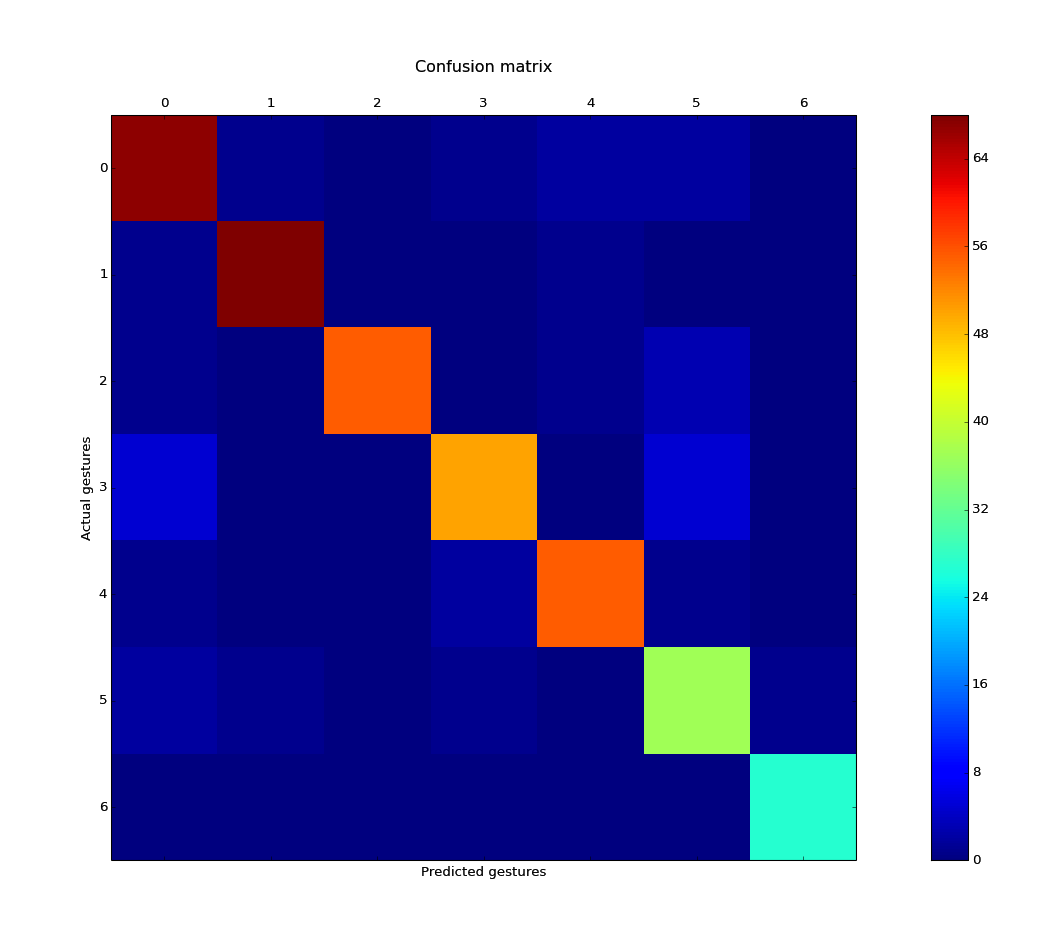
\includegraphics[width=0.3\textwidth]{svm/svm_confusion_matrix.png}
    \caption{Visuelle Darstellung einer Confusion Matrix}
    \label{fig:svm_confusion_matrix}
\end{figure}
\begin{table}[h]
\centering
\begin{tabular}{lrr}
\hline
 \multicolumn{1}{c}{\textbf{Gesture}} & \multicolumn{1}{c}{\textbf{Prec.}} & \multicolumn{1}{c}{\textbf{Recall}} \\
 \hline
  0: \texttt{\ac{RLO}} & 87\% & 92\% \\
 \hline
  1: \texttt{\ac{TBO}} & 97\% & 97\% \\
 \hline
  2: \texttt{\ac{OT}} & 100\% & 92\% \\
 \hline
  3: \texttt{\ac{SPO}} & 93\% & 83\% \\
 \hline
  4: \texttt{\ac{DPO}} & 93\% & 93\% \\
 \hline
  5: \texttt{\ac{RO}} & 77\% & 88\% \\
 \hline
  6: \texttt{\ac{BNS}} \& \texttt{\ac{BNN}} & 96\% & 100\% \\
 \hline
  Average & 92\% & 92\% \\
 \hline
\end{tabular}
\caption[Erkennungsraten einer SVM]{Erkennungsraten einer SVM}
\label{tab:svm_performance}
\end{table}
Durch die Wahl der in \autoref{sec:svm_training} vorgestellten Parameter wird die Fehlerrate in der Validierung auf insgesamt durchschnittlich 8\% minimiert.
Obwohl meist eine allgemeinere Klassifikation ohne Overfitting gewünscht ist, zeigt sich beim Testen der Live-Klassifikation ein ähnliches Bild.
So werden die meisten ausgeführten Gesten der korrekten Klasse zugeordnet.

\subsubsection{Fazit}\label{sec:svm_conclusion}
\ac{SVM}s zeigen, dass sie selbst bei der Verwendung von einer recht niedrigen Anzahl von verwendeten Trainingsdaten in der Lage sind, gute Klassifikationsergebnisse zu erzielen.
Weitere Vorteile von \ac{SVM}s bestehen darin, dass die Trainingsphase schnell absolviert und durch die Wahl entsprechender Parameter direkt Einfluss auf die Validierungsergebnisse genommen werden kann.
So liefert der trainierte \ac{SVM}-Klassifikator sehr gute Ergebnisse in der Validierung, da die Fehlerrate auf 8\% minimiert werden konnte.
Ausgenommen von zwei Gesten zeigte es sich ebenfalls, dass die Performance in der Live-Klassifikation trotz vermeintlichem Overfitting erstaunlich gut ist.
Bei den zwei Gesten, die nicht immer zuverlässig erkannt werden, handelt es sich um Geste 2 \texttt{\ac{OT}} und Geste 5 \texttt{\ac{RO}}.

Allgemein lässt sich die Performance des Klassifikators vor allem durch eine gute Vorverarbeitung und Merkmalsextraktion positiv beeinflussen.
Allerdings erschweren qualitativ unterschiedlich gute Trainingsdatensätze die Vorverarbeitungs- und die Trainingsphase und beeinflussen somit stark die Validierungs- und die Live-Klassifikationsergebnisse
Ursache dafür sind vermutlich die verschiedenen Laptops mit ihrer unterschiedlichen verbauten Hardware bezüglich Lautsprecher und Mikrofon.
Auch das nicht korrekte Ausführen der Gesten bei der Aufnahme für das Erstellen der Trainingsdatensätze ist eine Fehler- bzw. Problemquelle.
So erfordert die aktuelle Vorverarbeitungsstrategie eine recht exakte Ausführung der Geste unter sehr guten Vorraussetzungen.
Laute Umgebungsgeräusche sollten vermieden werden (dies kann jedoch auch an der aktuellen Hardwarekonfiguration des Testgeräts liegen), da das Mikrofon überempfindlich reagiert und teilweise selbst normale Musik oder Umgebungsgeräusche Schwankungen im Frequenzspektrum rund um die Referenzfrequenz von $18\text{,}5\text{ kHz}$ verursacht.

\clearpage
\section{\acl{HMM}}
\textit{Paul Pasler, Sebastian Rieder}

Das \acl{HMM} ist ein stochastisches Modell für sequentielle Daten und wird vor allem in der Spracherkennung und in der Bioinformatik eingesetzt.

In den folgenden beiden Abschnitten werden die Entstehung und Konzepte der \acl{MK} und des \acl{HMM} aufgezeigt.
Abschnitt \ref{sec:preproc} befasst sich mit der Aufbereitung der Daten für das Training und die Klassifizierung der Gesten.
Die Implementierung und Anwendung des \acl{HMM} werden im Abschnitt \ref{sec:impl} näher erläutert. Im letzten Abschnitt werden die Ergebnisse 
evaluiert und ein Fazit mit Ausblick gezogen. 
 
  %%%%%%%%%%%%%%%%%%
  %  MARKOV-KETTE  % 
  %%%%%%%%%%%%%%%%%%
\subsection{\acl{MK}} \label{sec:chain}
Grundlage des \acl{HMM} war die vom russischen Mathematiker Andrej Andrejewitsch Markov 
(1856 - 1922, siehe \cite{wiki:markov}) entwickelte \acl{MK}. Zu Beginn des 20. Jahrhunderts 
beschäftigte er sich als erster mit einer statistischen Beschreibung von Zustands- und Symbolfolgen. 
Er führte eine statistische Analyse der Buchstabenfolge des Textes ``Eugen Onegin'' von Alexander 
Pushkin.

Eine \acl{MK} ist eine Sequenz von Zufallsvariablen \( X_1, x_2, X_3, \ldots\) und beschreibt einen speziellen stochastischen Prozess, 
der aufgrund der Vorgeschichte, Aussagen über die Zukunft machen kann. 
Eine \acl{MK} kann als Gerichteter Graph mit Zuständen \(S\) und mit Übergangswahrscheinlichkeiten \(X_i\) an den Kanten beschrieben werden. 

Sie ist definiert durch eine endlich Menge an Zuständen \( S = \{ s | 1 <= s <= N \} \) und der diskreten Zeit \( t = 0, 1, 2, \ldots \) \\

\textbf{1. Markov Eigenschaft: } \\
\( \forall t \in \mathbb{N} : P (X_t = x_t | X_1 = x_1 ; \ldots ; X_{t-1} = x_{t-1} ; Y_1 = y_1 ; \ldots ; Y_{t-1} = y_{t-1} ) = P (X_t = x_t | X_{t-1} ) \) \\
Dies bedeutet, dass die \acl{MK} Gedächtnislos ist!


Eine \acl{MK} ist \cite[48]{mmmFink}:
\begin{itemize}
     \item \textit{stationär} \\
           Die Wahrscheinlichkeiten sind unabhängig von der Zeit
     \item \textit{kausal} \\
           Die Verteilung der Zufallsvariable \( S(t)\) hängt nur von den vergangenen Zuständen ab
     \item \textit{einfach} \\
           Die Abhängigkeiten der Prozesseingenschaften beschränken sich nur auf den unmittelbaren Vorgänger (1. Markov Eigenschaft) 
\end{itemize}
Bei einer \acl{MK} 1. Ordnung benötigt man für diese Aussagen nur den gegenwärtigen Zustand, um auf den nächsten Schritt zu schließen.



  %%%%%%%%%%%%%%%%%%
  %  HIDDEN-MARKOV  % 
  %%%%%%%%%%%%%%%%%%
\subsection{\acl{HMM} und \acl{GMM}}  \label{sec:hmm}
Der amerikanischen Mathematiker Leonard E. Baum (* 1931) und andere Autoren entwickelten auf Basis der \acl{MK} Ende der 
sechziger Jahre das \acl{HMM}. Erste \acl{HMM}-Applikationen wurden zur Spracherkennung und später auch in der Bioinformatik 
zur Analyse von Nukleotid- und Proteinsequenzen eingesetzt. 

Ein \acl{HMM} erweitert eine \acl{MK} um eine weiteren Zufallsprozess und ist somit ein zweistufiger stochastischer Prozess \cite[67]{mmmFink}
zustandsspezifische Ausgabe und eine statistisch modellierte Zustandsfolge. 


Es wird beschrieben durch:\\ 
\( \lambda = (S;V;A;B;\pi)\)
\begin{itemize}
     \item Endlich Menge von Zuständen \\
           \( S = \{ s | 1 <= s <= N \} \)
     \item Alphabeth der Emissionen \\
           \( V = \{ v | 1 <= v <= M \} \)
     \item Matrix der Zustandsübergangswahrscheinlichkeiten \\
           \( A = \{ a_{ij} | a_{ij} = P(S_t = j | S_{t-1} = i) \} \)
     \item Matrix der Emissionswahrscheinlichkeiten \\
           \( B = \{ b_{jk} | b_{jk} = P(O_t = o_k | S_t = j) \} \)
     \item Vektor von Zustandsstartwahrscheinlichkeiten \\
           \( \pi = \{ \pi_i | \pi_i = P(S_1 = i) \} \) 
\end{itemize}

Das Konzept des \acl{HMM} kann laut \cite{rabiner} in drei Problemstellungen eingeteilt werden:
\begin{itemize}
  \item Evaluierungsproblem: 
  \item Dekodierungsprobem: Finde interne Abläufe für eine gegebene Observationsfolge
  \item Trainingsproblem: Finde Modellparameter für gegebene Besispieldaten
\end{itemize}




Um das Training und die Klassifizierung möglichst genau und perfomant umzusetzen, 
ist es notwendig die aufgenommenen Daten auzubereiten, dies ist Thema des nächsten Abschnitts


  %%%%%%%%%%%%%%%%%%%
  %  PREPROCESSING  % 
  %%%%%%%%%%%%%%%%%%%
\subsection{Datenaufbereitung} \label{sec:preproc}
Eine Aufnahme wird beschrieben durch ein zwei-dimensionales Array aus 32 Frames mit jeweils 64 Frequenzwerten.
Im Ruhezustand bildet sich ein Signalpeak um die ausgesendete Frequenz (18.500hz).
Ziel ist es die Daten zu normieren und die Datenmenge zu reduzieren, um das Trainingergebnis bzw. Performance zu verbessern.
Weiterhin wird versucht die relevanten Werte einer Geste aus der Aufnahme zu extrahieren.

Da sich Änderungen durch eine Bewegung sehr Nahe am gesendeten Signal liegen, werden die Daten im 
Frequenzbereich von 18.000hz bis 19.000hz betrachtet, die Daten vermindern sich von 64 auf 13 Werte. 
Dazu wird jede Geste auf einem Intervall von 0 bis 1 normalisiert (Geteilt durch den jeweiligen Maximalwert) und 
auf zwei Nachkommstellen gerundet. 
Alle Werte unterhalb eines Schwellwerts (0.1) werden zudem abgeschnitten, um niedrig amplitudiges Rauschen zu vermindern. 
So wird im Idealfall nur das gesendete Signal und Frequenzänderungen durch eine Geste dargestellt.

Wichtig ist nun den Beginn und das Ende einer Geste zu finden. Hierzu werden pro Frame alle Werte addiert 
und das Maximum als Mittelpunkt der Geste genutzt. Von diesem Gestenhöhepunkt werden jeweils 6 Frames davor und danach mitgenutzt.

So wird aus einem 32 x 64 Array pro Geste ein 13x13 Array.


  %%%%%%%%%%%%%%%%%%%%%
  %  IMPLEMENTIERUNG  % 
  %%%%%%%%%%%%%%%%%%%%%
\subsection{Implementierung}  \label{sec:impl}
Wir haben uns für die scipy HMM implementierung entschieden. 
Genutzt wird ein \acl{HMM} mit \acl{GMM} entschieden.


  %%%%%%%%%%%%
  %  RESULT  % 
  %%%%%%%%%%%%
\subsection{Evaluation und Fazit}  \label{sec:result}
Das Hidden Markov Modell eignet sich grundsätzlich sehr gut für die gestellte Aufgabe. Da es mit sequenzielle Daten (Frames) umgehen 
kann und ursprünglich für die Spracherkennung entwickelt wurde. Ob nun aus einem Tonsignal (versteckte Zustände) ein Wort oder 
eine Geste (Emissionen) erkannt werden soll, ist vom Vorgehen ähnlich. Ein Vorteil ist zudem, dass die Ausführungsgeschwindigkeit
 der Geste, bei geeigneter Aufnahmelänge, die Klassifizierung nicht unbedingt beeinflusst, da dann länger im selben versteckten 
 Zustand verblieben wird.
Ein Nachteil dieser Methode ist, dass keine absoluten Klassifizierungen durchgeführt werden können. Es werden nur Wahrscheinlichkeiten für alle möglichen Klasse berechnet. So muss entschieden werden, ob die Wahrscheinlichkeit für eine Klasse hoch genug ist, sodass diese als Geste identifiziert werden kann.
\clearpage
\section{k-Means}
\textit{Alex Baumgärtner, Robert Brylka}

%\subsection{Hintergrund (Motivation/Geschichtliches)}

Der Begriff k-Means bezeichnet einen Clustering-Algorithmus von Stuart P. Lloyd \cite{Lloyd}, der 1957 entwickelt und erst 1982 in einer Fachzeitschrift veröffentlicht wurde. Unter Clustering versteht man hierbei die Gruppierung von Daten mit ähnlichen Eigenschaften in gleiche Klassen. Die Berechnung der optimalen Lösung eines solchen Klassifikationsproblems ist NP-schwer \cite{kMeansNPhard}. Aus diesem Grund sind Heuristiken wie k-Means hilfreich, um dennoch in angemessener Zeit eine akzeptable Lösung zu finden.
Ein solches Verfahren gehört zur Obergruppe des unüberwachten Lernens, bei denen die Trainingsphase durchlaufen wird, ohne dass Informationen über die zu den jeweiligen Daten passenden Klassen vorliegen.



\subsection{Funktionsweise des Klassifikators (Allgemein)}
%benötigt numerische Attribute, k muss vorher festgelegt werden
Der Algorithmus segmentiert eine Datenmenge in\emph{ k }verschiedene Cluster, indem\emph{ k }Cluster-Schwerpunkte berechnet werden und ein zu klassifizierendes Objekt immer dem nächstgelegenen Cluster-Schwerpunkt zugeordnet wird.

Der beschriebene Algorithmus arbeitet schnell und effizient, findet jedoch im besten Fall nur ein lokales Optimum. Unter bestimmten Bedingungen konvergiert der k-Means Algorithmus jedoch nicht einmal zum lokalen Optimum\cite{kMeansMinimum}. Aus diesem Grund ist es hilfreich, die Lernphase mehrere Male zu wiederholen und anschließend den Klassifikator mit der geringsten Fehlerquote zu benutzen.  


Der Algorithmus läuft folgendermaßen ab \cite{Marsland}:
\begin{itemize}

\item \emph{Initialisierung:} Es wird ein geeigneter Wert \emph{k} für die Anzahl der zu findenden Cluster gewählt. In Abschnitt XX wird darauf eingegangen, wie ein solches \emph{k} gewählt werden kann. Anschließend werden \emph{k} zufällige Positionen im Eingaberaum gewählt und jeweils als Cluster-Zentren festgelegt.
\item \emph{Lernvorgang:} Für jeden Datenpunkt wird der Abstand zu allen Cluster-Zentren berechnet und anschließend der Datenpunkt dem Zentrum mit dem geringsten Abstand zugeordnet. Danach 
Danach wird jedes Cluster-Zentrum in den Mittelpunkt aller ihm zugeordneten Punkte verschoben.
werden die Cluster-Zentren 
zur Mitte aller zugeordneten Punkte verschoben.
so verschoben, dass die Summe der Abstände aller zugeordneten Punkte minimal ist. 
Der gesamte Lernvorgang wiederholt sich solange, bis sich die Position der Cluster-Zentren nicht mehr verändert. 
\item \emph{Benutzung:} Um das passende Cluster zu einen Datenpunkt zu bestimmen, wird dessen Abstand zu allen Cluster-Zentren berechnet. Das Cluster, dessen Zentrum den geringsten Abstand hat, wird dem Datenpunkt zugeordnet.
\end{itemize}

K-Means benötigt in der Regel beim Lernen mehr Zeit als bei der Benutzung, da im ersten Fall die Cluster-Zentren unter Umständen oft verschoben werden müssen und nach jeder Verschiebung erneut die Abstände zu allen dem Zentrum zugeordneten Punkten berechnet werden müssen. Bei der Benutzung hingegen genügt es, nur die Abstände des zu klassifizierenden Punkts zu allen Cluster-Zentren zu berechnen, um das passende Cluster zu bestimmen. Der Algorithmus arbeitet jedoch im Vergleich zu anderen Klassifikatoren (TODO Beispiel??) in beiden Phasen schnell, da immer nur einfache Berechnungen des euklidischen Abstands im Eingaberaum erfolgen.

Es existieren weiterhin einige Variationen des Basis-Algorithmus, mit dem dieser weiter optimiert werden kann. Dazu gehört etwa ein vorzeitiger Abbruch des Lernens, wenn eine festgelegte Maximalzahl von Iterationen erreicht wurde. Mit dem k-Means++ Algorithmus \cite{kMeans++} kann die Dauer der Lernphase verkürzt und die Fehlerrate bei der Benutzung gesenkt werden. Dieser Algorithmus wird in der Initialisierungsphase zur Bestimmung der Startpositionen der Cluster-Zentren verwendet. 
%TODO k-Means++ genauer beschreiben




Wahl von optimalen Wert für k, in diesem Anwendungsfall (natürlich) mindestens Anzahl der Gesten, aber auch größere Werte möglich. Im einfachen Fall \emph{k} = AnzahlGesten wird jedem Clustercenter eine Geste zugeordnet. Im Idealfall wenig Überlappung der Confusion Matrix, sodass bei jeder Geste ein eindeutiges Cluster am häufigsten vorkommt und umgekehrt in jedes Cluster eine einzige Geste am häufigsten fällt (TODO: Später bei\emph{ k }> AnzahlGesten muss das nicht für jedes Cluster gelten, aber mindestens für\emph{ k }Stück). Wenn\emph{ k }größer ist als die Anzahl der Gesten, sind mindestens einer Geste mehrere Cluster-Schwerpunkte zugeordnet. --> Algorithmus, um Clustercenter den einzelnen Gesten zuzuordnen. 

\subsection{Anwendung auf Projekt}


\subsubsection{Datenaufbereitung}
Die Anzahl der zu bestimmenden Cluster (der Wert von k) muss bereits vor der Trainingsphase festgelegt werden. Dabei muss\emph{ k }mindestens gleich der Anzahl der Gesten sein, damit der Algorithmus in der Lage ist, die einzelnen Gesten voneinander zu unterscheiden. Zur Erkennung des Grundrauschens gibt es zwei Möglichkeiten: Entweder eine oder mehrere „Bullshit-Klassen“ einführen, die Aufnahmen entsprechen, bei denen keine (bekannte) Geste ausgeführt wurde. Die zweite Möglichkeit ist, den maximalen Abstand einer Geste zum nächstgelegenen Cluster-Center zu begrenzen, sodass beim Überschreiten des Grenzwerts „keine Geste“ klassifiziert wird.
2 Cluster für Hintergrundrauschen, eins für leise und eins für laute Umgebung
Ziel: Besser eine Geste fälschlicherweise als Grundrauschen einstufen und nicht erkennen, als das Grundrauschen oder andere Bewegungen beim Bedienen des Rechners als Geste einstufen. Im ersten Fall wird der Anwender die Geste einfach erneut ausführen (und sie wird dann – hoffentlich – auch erkannt), im zweiten Fall ist es nervig, da die mit der erkannten Geste verknüpfte Aktion ausgeführt wird. 

Rohdaten sind zu hochdimensional, um ohne Vorverarbeitung in den Klassifikator gesteckt werden zu können. Bei der verwendeten Implementierung (siehe später) sind pro Geste beispielsweise 32 Frames $\cdot$ 64 Lautstärkewerte, die je einem Frequenzbereich entsprechen (siehe FFT \cite{fftMathebuch}), = 2048 Daten vorhanden. Da hochdimensionale Eingabedaten bei Clustering-Verfahren oft schlechte Ergebnisse liefern \cite{kMeansHighDimensions}, ist es notwendig, bei der Datenaufbereitung die Dimension der Eingabedaten zu reduzieren. Erste Tests mit nicht aufbereiteten 2048-dimensionalen Eingabedaten lieferten eine korrekte Erkennungsrate von etwa 25 bis 30 Prozent bei 6 Klassen (5 Gesten sowie Grundrauschen ohne Geste). Lediglich das Grundrauschen kann einigermaßen zuverlässig erkannt werden, eine korrekte Unterscheidung der einzelnen Gesten ist jedoch war jedoch nicht möglich. Dies zeigt deutlich die Notwendigkeit einer Datenaufbereitung.


\subsubsection{Anpassung des Klassifikators}
Bei dem k-Means Algorithmus ist zu beachten, dass die Anzahl der Cluster vorher bekannt sein muss, da sie beim Start des Algorithmus festgelegt wird. Dies ist jedoch kein Problem, weil die Anzahl der Gesten im Erkennungssystem auf eine bestimmte Zahl (voraussichtlich 6) festgelegt ist. Da der Klassifikator jede beliebige Eingabe einem der Cluster zuordnet, ist es notwendig, eine oder mehrere zusätzliche Gruppen für nicht erkannte Gesten zu definieren. Ansonsten würde jede Eingabe – unabhängig ob es tatsächlich eine Geste war oder nicht – grundsätzlich der ähnlichsten bekannten Gesten zugeordnet. Denkbar sind hierbei beispielsweise zwei solcher zusätzlicher Gruppen, eine für das Hintergrundrauschen ohne Bewegung und eine weitere für alle Bewegungen, die keiner gespeicherten Geste entsprechen.
Die Features zur Klassifikation müssen so gewählt werden, dass sich gleiche Gesten im gleichen Cluster anordnen und es möglichst nicht zu einer Überschneidung von verschiedenen Clustern kommt. Dies ist notwendig, da der Klassifikator ansonsten nicht mehr in der Lage ist, die einzelnen Gesten voneinander zu unterscheiden. Anhand des im aktuellen Prototyp dargestellten Frequenzspektrums lässt sich erkennen, dass sich die Gesten weniger durch die zu einem bestimmten Zeitpunkt gemessenen Frequenzwerte unterscheiden lassen, sondern eher durch den zeitlichen Verlauf dieser Frequenzwerte von Beginn bis Ende der Geste.


\subsubsection{Implementierung}
Die Implementierung erfolgte in der Programmiersprache Python unter Verwendung der Bibliothek skikit-learn (Version 0.14) \cite{sklearn}. Diese Bibliothek verwendet den beschriebenen k-Means Algorithmus von Lloyd. Außerdem bietet sie noch die Möglichkeit, dass die Startpunkte der Cluster-Center nicht wie im ursprünglichen Algorithmus vorgesehen zufällig gewählt werden, sondern stattdessen mit dem k-Means++ Algorithmus \cite{kMeans++} bestimmt werden. Zusätzlich können noch weitere kleine Einstellungen vorgenommen werden, um den Klassifikator für den jeweiligen Anwendungsfall  zu optimieren. Dazu gehört beispielsweise eine Beschränkung der Iterationen beim Lernen auf einen bestimmten Maximalwert.
Die Komplexität im ungünstigsten Fall liegt bei $O(n^{(k+2)/p})$ \cite{kMeansHowSlow}, wobei $n$ der Anzahl der Trainingsdaten und $p$ der Anzahl der Dimensionen entspricht.


\subsubsection{Training}
Zu Beginn der Lernphase des Algorithmus wird ein Wert für\emph{ k }festgelegt und anschließend werden\emph{ k }zufällige Positionen im Eingaberaum als Cluster-Schwerpunkte gesetzt (Abbildung XX). Danach wird jeder Schwerpunkt so verschoben, dass der Abstand zwischen ihm und den zugeordneten Objekten einen minimalen Wert annimmt. Diese Verschiebungen werden solange wiederholt, bis sich die Cluster-Schwerpunkte nicht mehr bewegen. 
Um nun zu einem Objekt den passenden Cluster zuzuordnen, wird der Abstand zwischen Objekt und den Cluster-Schwerpunkten berechnet. Das Objekt wird dann dem Cluster-Schwerpunkt mit dem geringsten Abstand zugeordnet. Abbildung XX zeigt eine solche Bestimmung anhand der zuvor berechneten Cluster-Schwerpunkte. Die Zugehörigkeit beliebiger Objekte zu den jeweiligen Cluster-Centern ist farbig markiert, sodass ein zu klassifizierendes Objekt das der Farbe entsprechende Cluster zugeordnet wird.
k-Means ist anfällig für Ausreißer
Wahl eines guten Werts für\emph{ k }von Bedeutung, offensichtlich mindestens Anzahl der Gruppen (wenn Anzahl der Gruppen vorher bekannt ist). Verschiedene Methoden, die einfachste ist die Faustregel, dass $k \approx \sqrt{n/2}$ (REF).
%Quelle:  Faustregel: Kanti Mardia et al. (1979). Multivariate Analysis. Academic Press. (via http://en.wikipedia.org/wiki/Determining_the_number_of_clusters_in_a_data_set)


\subsubsection{Evaluation}
Confusion Matrix in lauter und leiser Umgebung für die verschiedenen Gesten. Welche Gesten werden sehr gut/gut/mittelmäßig oder gar nicht erkannt? Erkennungsrate praxistauglich?



\subsection{Fazit}
Die Erkennung funktioniert mittelmäßig/gut/sehr gut. Sehr gut erkannt werden das Grundrauschen und Geste(n) XX. Schlecht/kaum erkannt werden Geste(n) XX (siehe Confusion Matrix). Ausblick auf potentielle weiterführende Arbeiten
\clearpage
\section{Entscheidungsbäume, Boosting und Bagging}
\textit{Annalena Gutheil, Matthias Volland}

Die Verwendung von baumartigen Strukturen zur Klassifikation von Daten bietet sich aus mehreren Gründen an. 
%Einerseits handelt es sich bei Bäumen um eine Datenstruktur, die häufig in der Informatik verwendet wird und daher vom Verständnis intuitiver ist, als beispielsweise ein neuronales Netzwerk oder eine SVM. 
Einerseits handelt es sich bei Bäumen um eine Datenstruktur, die häufig in der Informatik verwendet wird. Durch ihre nachvollziehbare hierarchische Struktur, sind sie vom Verständnis intuitiver als beispielsweise eine neuronales Netz.
Andererseits ist das Erzeugen von Bäumen im Allgemeinen relativ effizient, was bei Machine-Learning-Algorithmen 
in der Traningsphase wichtig ist. Das Verwenden bzw. Durchlaufen eines Baumes hat lediglich eine logarithmische Komplexität, 
so dass auch die Klassifikation durch einem Baum sehr effizient ist, sofern dieser nicht entartet ist. 

\subsection*{Entscheidungsbäume}

Bäume zur Klassifikation von Daten werden auch als \glqq Entscheidungsbäume\grqq\ bezeichnet und bestehen aus Knoten, Kanten und Blättern. Knoten entsprechen dabei Merkmalen bzw. \glqq Features\grqq\ der zu klassifizierenden Daten und die Kanten an einem Knoten den verschiedenen Merkmalsausprägungen. 
Ein Knoten kann entweder einen weiteren Knoten als Kind haben (also ein weiteres Merkmal) oder aber ein Blatt, was einer Klasse entspricht.

Um beispielsweise verschiedene Gemüsesorten zu klassifizieren, könnten im einfachsten Fall Farbe und Form als Unterscheidungsmerkmale dienen. Wenn jedes Objekt der Testmenge die Merkmale (Form, Farbe) hat, würde eine Tomate mit (rund, rot) beschrieben, eine Gurke mit (länglich, grün) und eine Möhre mit (länglich, orange).

Ein Entscheidungsbaum zur Klassifikation könnte dann aus einem Wurzel-Knoten bestehen, der zunächst anhand der Form 
des zu klassifizierenden Objektes eine erste Entscheidung vornimmt. Da eine Tomate rund ist und Gurken und Möhren länglich, 
hätte der Wurzelknoten zur Unterscheidung der Form die beiden Kanten \glqq rund\grqq\ und \glqq länglich\grqq\ . Da in dem Beispiel nur Tomaten rund sind, hätte die Kante mit dem Attribut \glqq rund\grqq\ das Blatt bzw. die Klasse \glqq Tomate\grqq\ als Kind. Gurken und Möhren haben 
jedoch beide eine längliche Form, so dass diese nicht alleine aufgrund der Form unterschieden werden können. Daher müsste die 
Kante mit dem Merkmal \glqq länglich\grqq\ in einen weiteren Knoten münden, durch welchen die Testmenge in einem nächsten Schritt anhand der Farbe weiter unterteilt werden müsste. Dieser Entscheidungsknoten hätte die Kanten \glqq rot\grqq , \glqq grün\grqq\ und \glqq orange\grqq, die jeweils in einem Blattknoten mit den Klassen \glqq Tomate\grqq , \glqq Gurke\grqq\ und \glqq Möhre\grqq\ müden würden.

In dem Beispiel hätte als erstes Unterscheidungsmerkmal auch die Farbe dienen können, wodurch direkt in einem Schritt alle drei Gemüsesorten hätten klassifiziert werden können. Somit hat die Wahl der Reihenfolge der Merkmale einen wesentlichen Einfluss auf die Form des Entscheidungsbaumes sowie die Effizienz, mit der Testdaten klassifiziert werden können. Weiterhin können durch die ungünstige Wahl von Kriterien verschiedene Klassen mehrfach in dem Entscheidungsbaum vorkommen, was darauf schließen lässt, dass der Baum aufgrund der Redundanz mehr Knoten enthält, als für eine Klassifizierung notwendig wäre.

Es gibt verschiedene Kriterien, nach denen die Reihenfolge der Merkmale so gewählt werden kann, dass ein möglichst kompakter und damit effizienter Entscheidungsbaum entsteht. Ein Ansatz besteht darin zu berechnen, wie groß der Informationsgehalt der zu unterscheidenden Merkmale ist. Der Informationsgehalt eines Merkmals bestimmt sich daraus, wie häufig es vorkommt und ist definiert als 
\[I = -log(p_i)\] wobei $p_i$ die relative Häufigkeit ist, mit der das Merkmal $i$ vorkommt. Ein sehr häufig vorkommendes Merkmal hat dementsprechend einen niedrigeren Informationsgehalt als ein seltenes Merkmal. Der Mittlere Informationsgehalt aller Merkmale wird auch als Entropie bezeichnet lässt sich dann mit Hilfe der Formel 
\[E = - \sum \limits_{i=1}^n p_i \cdot \log (p_i)\] berechnen, wobei $n$ die Menge aller Merkmale ist und $p_i$ die relative Häufigkeit des Merkmals $i$.
Um nun das Vorkommen der Merkmale in Relation zu den möglichen Klassifikationen zu setzen, wird die bedingte Wahrscheinlichkeit für die Merkmale bezogen auf die möglichen Klassen ermittelt, woraus sich der mittlere Informationsgewinn ermitteln lässt. Dieser ist definiert als 
\[H = - \sum \limits_{i=1}^n p_i \cdot (\sum \limits_{j=1}^m \frac{x_{ij}}{x_i} \cdot \log (\frac{x_{ij}}{x_i}))\] wobei $n$ die Anzahl der Merkmale ist und $m$ die Anzahl der Klassen. Der Wert $x_i$ beschreibt die Anzahl der Vorkommen der Merkmalsausprägung $i$ und $x_{ij}$ die Anzahl der Vorkommen dieser Merkmalsausprägung unter der Bedingung, dass das Objekt zur Klasse $j$ gehört.
Beim Erstellen eines Entscheidungsbaumes ist dann das Merkmal für die Teilung am interessantesten, was den größten mittleren Informationsgewinn H hat, also die innere Summe minimal ist.
Da sich durch das Merkmal \glqq Farbe\grqq\ aus dem vorigen Beispiel direkt alle möglichen Klassen unterscheiden lassen, hat dieses Merkmal z.B. einen höheren Informationsgewinn als das Merkmal \glqq Form\grqq\ und bietet sich daher als erstes Entscheidungskriterium an.

Ein anderes Maß zur Auswahl von geeigneten Entscheidungsmerkmalen ist die sogenannte \glqq Reinheit\grqq\ von Merkmalen. Die Reinheit eines Merkmales ergibt sich daraus, wie viele verschiedene Klassen die jeweiligen Merkmalsausprägungen beinhalten. Das Attribut \glqq Farbe\grqq\ aus dem vorigen Beispiel führt zu drei Blattknoten, bei denen durch jeden Knoten genau eine Klasse repräsentiert wird (nämlich jeweils die Klassen Tomate, Gurke und Möhre) während beim Merkmal \glqq Form\grqq\ sowohl Möhren als auch Gurken als mögliches Ergebnis in Frage kommen, falls das zu klassifizierende Objekt die Merkmalsausprägung \glqq länglich\grqq\ hat. Die Reinheit ist dementsprechend ein Maß dafür, wie groß das Risiko einer falschen Klassifikation ist. Ziel ist es anhand von Merkmalen Teilungen im Entscheidungsbaum vorzunehmen, die ein möglichst geringes Risiko für falsche Klassifikationen haben.

%Entscheidungsbäume funktionieren nach dem \glqq teile und herrsche\grqq\ -Prinzip. 
%Beginnend beim Wurzelknoten wird bei jedem Knoten mithilfe einer Testfunktion berechnet, welche Abzweigung genommen werden muss. 
%Ist man am Blattknoten angekommen, ist dies die zur Eingabe gehörende Klasse~\cite{alpaydin:maschinelles_lernen, borgelt:data_mining}.

\subsection{Ensemble Learning}
Die Idee von Ensemble Learning ist es, mehrere Klassifikatoren gleichzeitig zu verwenden anstatt eines einzigen Klassifikators, um bessere Ergebnisse zu erzielen. Der Vorteil bei der Verwendung mehrerer Klassifikatoren ist es, dass nicht ein einzelner Klassifikator alle Klassen möglichst gut unterscheiden können muss, sondern dass mehrere (unabhängig voneinander gesehen schwächere) Klassifikatoren zusammen einen starken Klassifikator bilden können. Wichtig ist dabei lediglich, dass jeder der schwachen Klassifikatoren geringfügig besser sein muss als raten, also bei einer binären Klassifikation eine Erfolgsrate von mehr als 50\% hat.
Bezugnehmend auf das einführende Beispiel zur Klassifikation verschiedener Gemüsesorten könnte man also beispielsweise einen Klassifikator verwenden, der sehr gut anhand der Form klassifizieren kann und einen weiteren anhand der Farbe. Ein Nachteil von Ensemble Learning ist jedoch, dass der Trainingsaufwand mit der Anzahl der Klassifikatoren steigt. Da bei Entscheidungsbäumen das Training verglichen mit anderen Klassifikatoren jedoch relativ effizient ist, bieten sich Entscheidungsbäume besonders als Klassifikatoren für Ensemble Learning an. Im Folgenden werden daher zwei verschiedene Ansätze des Ensemble Learning vorgestellt.


\subsection*{Bagging}
Eine einfache Methode, um mehrere Klassifikatoren miteinander zu kombinieren, wird als Bagging bezeichnet, eine Abkürzung für Bootstrap Aggregating. Der Name steht im Zusammenhang mit der Ziehung von Stichproben aus einer Menge, wo ein \glqq bootstrap sample\grqq\ eine Bezeichnung dafür ist, ein Testdatensatz \glqq mit Zurücklegen\grqq\ aus der Testmenge zu ziehen. Somit können manche Testdaten mehrfach, andere gar nicht in der Trainingsmenge vorhanden sein. Durch die daraus resultierenden unterschiedlichen Trainingsdaten entstehen Klassifikatoren, die verschiedene Klassen unterschiedlich gut unterscheiden können. Die Klassifikation erfolgt dann aufgrund einer Mehrheitsentscheidung.

\subsection*{Boosting}
Boosting unterscheidet sich zu Bagging dahingehend, dass während des Trainings immer mit den gleichen Trainings- und Testdaten gearbeitet wird und nicht eine zufällige Auswahl verwendet wird.
Das bekannteste Boosting-Verfahren heißt AdaBoost und existiert seit Mitte der 90er Jahre. Die grundsätzliche Idee bei dem Verfahren ist es, jeden Datensatz um ein zusätzliches Gewicht als Maß dafür zu erweitern, wie fehlerbehaftet dieser Datensatz in den vorigen Trainingsrunden klassifiziert worden ist. Durch dieses Gewicht, welches im Laufe der Klassifikation immer wieder angepasst wird, werden nicht richtig klassifizierte Daten hervorgehoben und stärker fokussiert. AdaBoost ist ein iterativer Algorithmus, der für jede neue Iteration die Fehlklassifikationen des vorherigen Trainings mit einbezieht mit dem Ziel, im besten Fall am Ende alle Testdaten richtig zuzuordnen. Das Gewicht berechnet sich anhand des jeweiligen Fehlers $\epsilon$, der sich aus der Summe der Gewichte der falsch klassifizierten Datenpunkte zusammensetzt. Das Gewicht dieser Datenpunkte wird mit
$ \alpha = \frac{\epsilon}{(1-\epsilon)} $ 
multipliziert, sodass die \glqq schwierig\grqq\ zu klassifizierenden Daten stärker berücksichtigt werden. Ziel ist es mit jedem weiteren Training einen neuen Klassifikator zu erhalten, der ein niedrigeren Fehler hat als in den vorangegangenen Iterationen. Die Trainingsphase kann dadurch beendet werden, dass eine feste Anzahl an auszuführenden Iterationen vorgegeben wird oder wenn das Optimum, dass alle Datenpunkte richtig klassifiziert wurden, erreicht wurde.

\subsection{Datenaufbereitung}
\label{sect:Trees_Datenaufbereitung}
Die zu klassifizierenden Gesten unterscheiden sich dahingehend, dass sie die Bandbreite 
des Frequenzspektrums um den Referenzton in unterschiedlicher Weise verschieben bzw. vergrößern. 
Um eine Geste zu erkennen, werden daher die Amplituden der aufgezeichneten Frequenzen 
um die Amplitude der Frequenz des Referenztons im Spektrum in beiden Richtungen analysiert. 
Relevant für die Erkennung der Gesten sind dabei im Allgemeinen nur diejenigen Frequenzanteile 
um den Referenzton, deren Amplitude den Grenzwert von 10\% der Amplitude des Referenztones nicht unterschreitet. 
In Ausnahmefällen können die Frequenzanteile einer Geste im Spektrum durch ein lokales Minimum vom Referenzton 
separiert sein. Daher wird zusätzlich nach einem weiteren Ausschlag im Spektrum gesucht, 
dessen Maximum mindestens 30\% der Amplitude des Referenztons entsprechen muss.


Eine Geste setzt sich zunächst aus 32 Einzelaufnahmen (Samples) zusammen, welche jeweils 
64 Amplitudenwerte beinhalten. Somit besteht eine Geste zunächst aus insgesamt 2048 Werten.
Da wie einführend beschrieben die Amplituden der Frequenzanteile einer Geste durch ein lokales Minimum vom Referenzton 
getrennt sein können, werden die Amplituden der einzelnen Samples zunächst mit einem Gauß-Filter geglättet, 
so dass größere Schwankungen aus dem Signal entfernt werden. 
Abbildung~\ref{fig:gauss} zeigt die Amplituden des Frequenzspektrums von einem Sample 
vor dem Glätten mit einem Gauß-Filter (rot) und danach (blau).

\begin{figure}[htbp] \centering
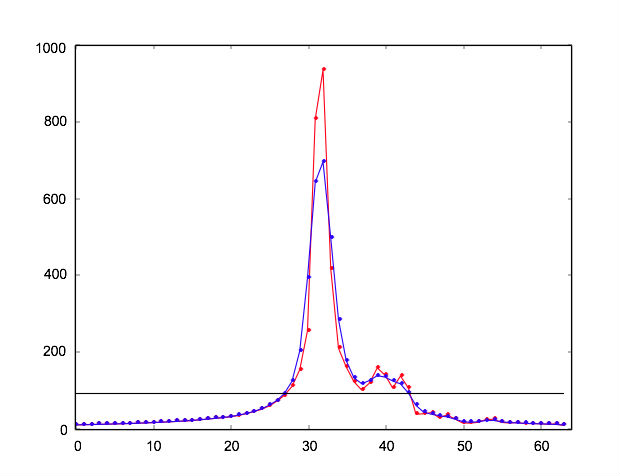
\includegraphics[height=60mm]{trees/gesture4-gauss1.jpg}
\caption{Rot: Ungefilterte Amplitudenwerte, Blau: Durch Gauß-Filter geglättete Amplitudenwerte}
\label{fig:gauss}
\end{figure}

Für die effiziente und robuste Klassifizierung der Gesten bietet es sich weiterhin an, 
die Komplexität der generierten Eingabedaten zu reduzieren. Dazu wird in jedem Sample einer Geste 
auf der linken und rechten Seite des Referenztons die Anzahl der Amplituden des geglätteten Signals ermittelt, 
deren Wert größer als 10\% ist. Der daraus resultierende Graph zeigt dann für eine Geste die zeitliche 
Änderung der Amplitudenanteile um den Referenzton auf der linken und rechten Seite an. Dieser Graph ist in Abbildung~\ref{fig:sum_of_bins} dargestellt, wobei die Anzahl der zum Referenzton gehörenden Amplituden aller Frequenzen unterhalb des
Referenztons in rot dargestellt sind, die Frequenzanteile oberhalb des Referenztons in blau.

\begin{figure}[htbp] \centering
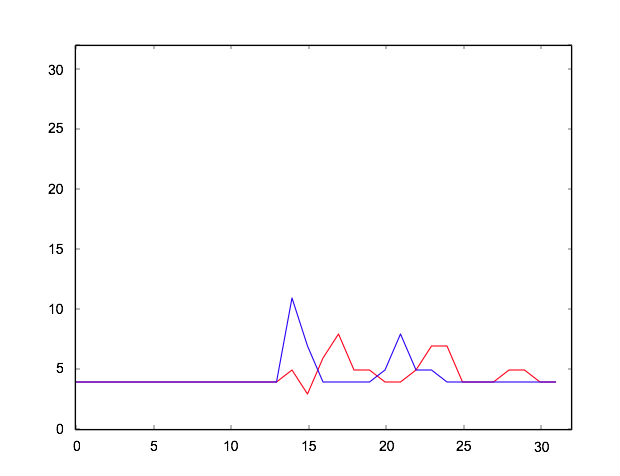
\includegraphics[height=60mm]{trees/gesture4-peaksize.jpg}
\caption{Frequenzanteile links (rot) und rechts (blau) von dem Referenzton}
\label{fig:sum_of_bins}
\end{figure}

Bei der in der Grafik dargestellten Geste handelt es sich um einen \glqq Double-Push\grqq , also eine Geste, bei der die Hand zwei mal 
hintereinander schnell auf den Monitor bzw. das Mikrofon zubewegt wird. Diese Geste äußert sich in jeweils zwei aufeinander folgenden 
Verschiebungen der Frequenzen nach rechts (auf den Monitor zu bewegen) und links (vom Monitor weg bewegen). 
Diese Charakteristik lässt sich in der Grafik erkennen, da die Anzahl der zum Referenzton gehörenden Frequenzanteile zunächst nach rechts (erster Peak blau) und dann nach links (zweiter Peak rot) ansteigt. Aufgrund des \glqq Double-Push\grqq\  erfolgt diese 
Verschiebung zwei mal hintereinander, so dass insgesamt vier Ausschläge (zwei nach rechts und zwei nach links) zu erkennen sind. 
Somit kann in einem Schritt die Anzahl der Daten pro zu klassifizierender Geste von 32\cdot 64=2048 Amplitudenwerten 
auf 2\cdot 32=64 reduziert werden, wobei diese Werte keinen Rückschluss auf die genauen Frequenzanteile zulassen sondern 
ein Maß dafür sind, wie sich die Frequenzanteile ober- und unterhalb des Referenztons verändern.

Die daraus entstehenden Daten können in einem weiteren Schritt geglättet werden, da nur Amplitudenschwankungen ab einer gewissen 
Größe auf eine ausgeführte Bewegung schließen lassen. Dazu werden alle Schwankungen auf der rechten oder linken Seite entfernt, 
die unterhalb eines definierten Grenzwertes liegen. 
Abbildung~\ref{fig:filtered} zeigt ein gefilterten Graph, in dem alle Ausschläge entfernt werden, die kleiner als 2 sind:

\begin{figure}[htbp] \centering
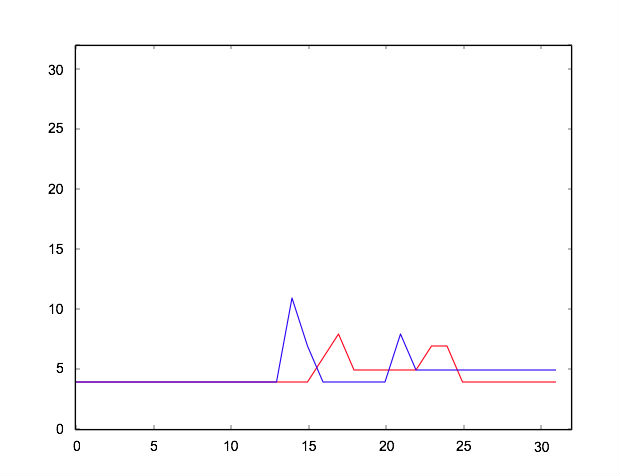
\includegraphics[height=60mm]{trees/gesture4-peaksize-smoothed.jpg}
\caption{Geglättete Frequenzanteile}
\label{fig:filtered}
\end{figure}

In einen dritten Schritt werden die Amplitudenwechsel dahingehend weiter geglättet, indem zunächst die Anzahl der am häufigsten 
auftretenden Frequenzanteile auf der linken und rechten Seite vom Referenzton ermittelt werden. Anschließend werden alle Werte,
die in einem vorher definierten Bereich ober- oder unterhalb dieses Wertes liegen auf den am häufigsten vorkommenden Wert gesetzt.
Dieser Schritt ist in Abbildung~\ref{fig:frequent_value} zu sehen, wobei alle Werte die +1 oder -1 um den häufigsten Wert verteilt sind 
auf den häufigsten Wert gesetzt wurden:

\begin{figure}[htbp] \centering
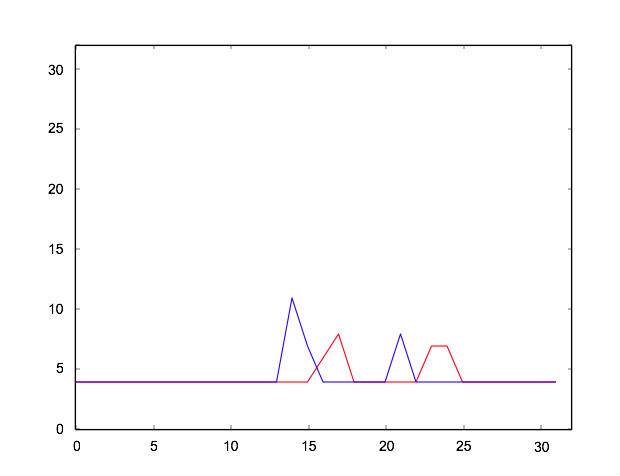
\includegraphics[height=60mm]{trees/gesture4-peaksize-smoothed2.jpg}
\caption{Geglätteter Graph anhand des am häufigsten vorkommenden Wertes}
\label{fig:frequent_value}
\end{figure}


Stark vereinfacht unterscheiden sich die Gesten dahingehend, ob und auf welcher Seite 
eine Veränderung der Anzahl aller zum Referenzton gehörenden Frequenzanteile stattfindet. 
Weiterhin muss unterschieden werden, in welche Richtung sich diese Verschiebung ausbreitet. 
Sie kann beispielsweise von der rechten zur linken oder von der linken zur rechten Seite 
um den Referenzton wandern, sowie gleichzeitig auf beiden Seiten stattfinden. 
Ein Beispiel dafür zeigt Abbildung~\ref{fig:left_right_same_time}

\begin{figure}[htbp] \centering
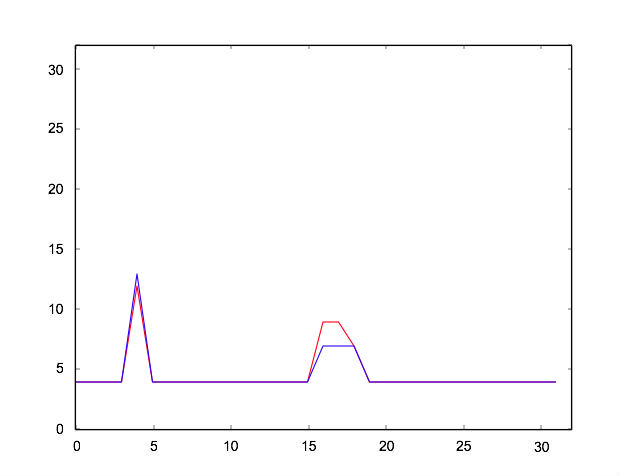
\includegraphics[height=60mm]{trees/gesture2-peaksize-smoothed2.jpg}
\caption{Gleichzeitige Verschiebung zur rechten und linken Seite des Referenztons}
\label{fig:left_right_same_time}
\end{figure}

Bei der in der Grafik abgebildeten Geste handelt es sich um ein mit der rechten und linken Hand entgegengesetztes zu und 
wegbewegen von dem Monitor, so dass gleichzeitig auf der rechten und linken Seite eine Vergrößerung der 
zum Referenzton gehörenden Frequenzanteile entsteht, was sich auch in der Grafik ablesen lässt.
Diese Unterscheidungsmerkmale können sehr gut durch einen Entscheidungsbaum abgebildet werden. 
Dazu kann die Verschiebungsrichtung als Maß dienen, um die Eingabemenge zu unterteilen und 
somit eine Klassifizierung zu erreichen.

\subsubsection{Charakteristiken der Gesten} \label{charakteristiken}
Durch die Vorverarbeitung der Daten entstehen für die einzelnen Gesten Charakteristiken, anhand dessen sie unterschieden werden können. 

%\paragraph*{Right-to-left}

%\paragraph*{Top-to-bottom}

\paragraph*{Two-hands-contrary}
Die in Abbildung~\ref{fig:contrary} dargestellten aufbereiteten Daten der Frequenzverschiebungen, die die Geste \glqq Two-hands-contrary\grqq\ erzeugt, zeigt üblicherweise je zwei gleichzeitige, also übereinander liegende, Frequenzverschiebungen. Dies ist dadurch zu erklären, dass zur selben Zeit eine Bewegung auf das Aufnahmegerät zu und von diesem weg durchgeführt wird.

\begin{figure}[htbp] \centering
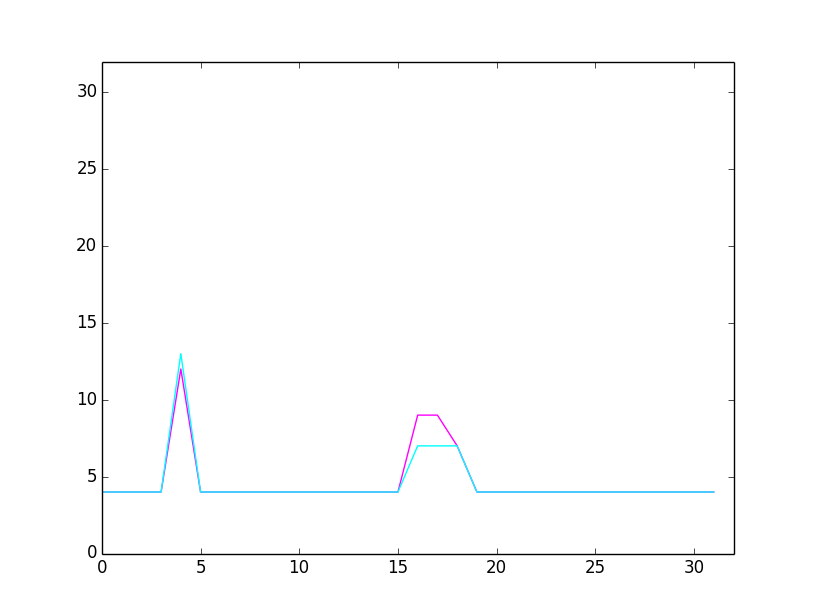
\includegraphics[height=60mm]{trees/contrary.png}
\caption{Two-hands-contrary}
\label{fig:contrary}
\end{figure}


\paragraph*{Single-Push}
Der \glqq Single-Push\grqq\ ist eine einfache Bewegung auf das Aufnahmegerät zu, sodass eine Frequenzverschiebung auf der rechten Seite des Frequenzspektrums festgestellt werden kann. Dies ist in Abbildung~\ref{fig:single_push} dargestellt.

\begin{figure}[htbp] \centering
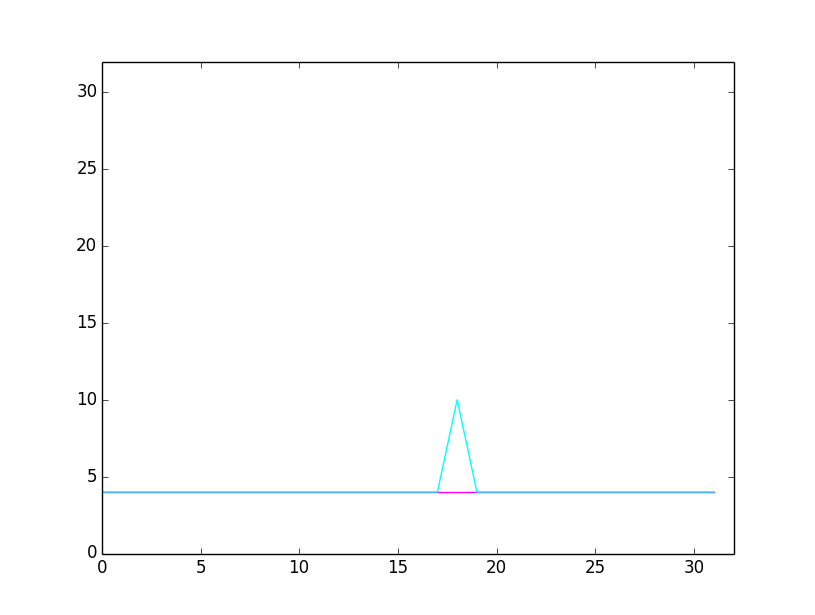
\includegraphics[height=60mm]{trees/single_push.png}
\caption{Single-Push}
\label{fig:single_push}
\end{figure}

\paragraph*{Double-Push}
Die charakteristischen Daten der Geste \glqq Double-Push\grqq\ ist in Abbildung~\ref{fig:double_push} abgebildet. Sie zeichnet sich durch je zwei Verschiebungen auf der rechten und auf der linken Seite aus. Die Rechts-Links-Verschiebungen treten dabei kurz hintereinander auf und können sich auch teilweise überlappen. 

\begin{figure}[htbp] \centering
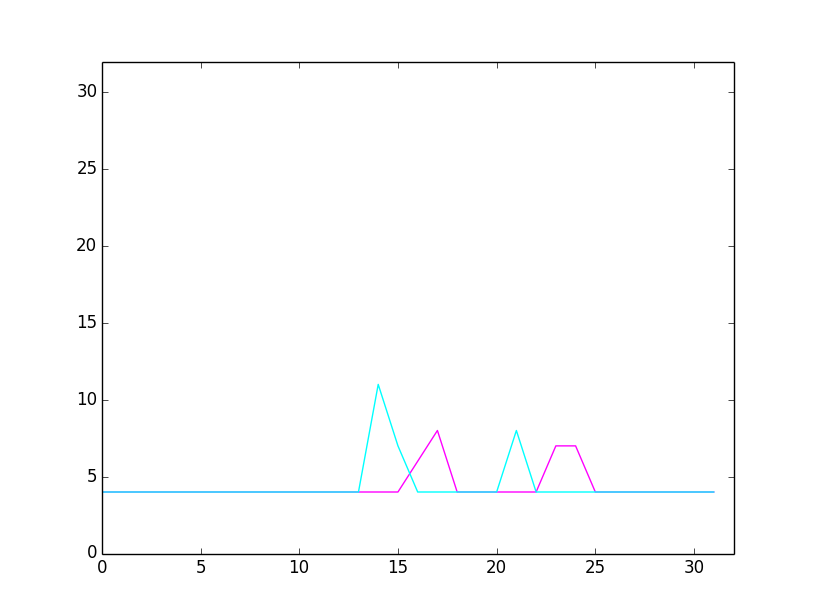
\includegraphics[height=60mm]{trees/double_push.png}
\caption{Double-Push}
\label{fig:double_push}
\end{figure}

\paragraph*{Nothing}
Um später Gesten live zu erkennen, muss auch definiert sein, wann keine Geste auftritt. In diesem Fall ist in Abbildung~\ref{fig:nothing} keine Frequenzverschiebung zu erkennen. Der Graph zeigt keinen Ausschlag.

\begin{figure}[htbp] \centering
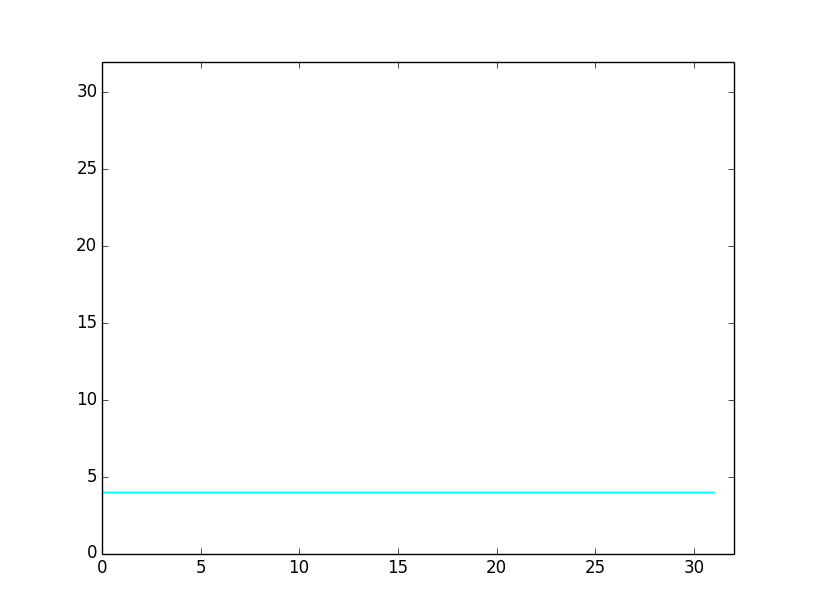
\includegraphics[height=60mm]{trees/nothing.png}
\caption{Keine Geste}
\label{fig:nothing}
\end{figure}

\subsection{Merkmalsextraktion}
Durch die Filterung und Glättung können nun die einzelnen Frequenzverschiebungen eindeutig identifiziert werden. Zudem ist in Abschnitt~\ref{charakteristiken} beschrieben, welche typische Gestalten der Graph für die verschiedenen Gesten annimmt. So lassen sich durch die Anordnung, Ausprägung und Aufkommen der Frequenzverschiebungen die unterschiedlichen Charakteristiken der einzelnen Gesten erkennen. Das Ziel der Merkmalsextraktion ist es, aus den 32 Datenpunkten weitere eindeutige Merkmale herauszuarbeiten um schließlich einen Merkmalsvektor mit überschaubarer Anzahl an Merkmalen zu generieren. Um dies zu realisieren, wurden folgende Eigenschaften der einzelnen Gesten untersucht:

\begin{itemize} 
\item Anzahl der Frequenzverschiebungen
\item Zeitliche Abfolge der Frequenzverschiebungen
\item Amplitudenunterschiede zwischen den Frequenzverschiebungen
\end{itemize}

\subsubsection*{Anzahl der Frequenzverschiebungen}
Die Anzahl der Frequenzverschiebung sagt bereits einiges über die Geste aus, wobei auch wichtig ist, ob die Frequenzverschiebungen im höheren oder niedrigeren Frequenzbereich liegen. Wie bereits in Abschnitt~\ref{sect:Trees_Datenaufbereitung} erwähnt, erzeugt eine Bewegung auf das Aufnahmegerät zu eine Frequenzverschiebung auf der rechten Seite, also eine Ausdehnung in Richtung der höheren Frequenzen. Durch das Bewegen vom Aufnahmegerät weg, erfolgt eine Frequenzverschiebung zur linken Seite, bzw. in Richtung der niedrigeren Frequenzen. 

Ein einfacher \glqq Single-Push\grqq\ erzeugt deshalb im optimalen Fall eine Frequenzverschiebung auf der rechten Seite des Peaks. Wird die Hand wieder zurückgezogen, tritt auch eine Frequenzverschiebung auf der linken Seite auf. Klar davon abgegrenzt werden kann beispielsweise die Geste \glqq Double-Push\grqq. Diese erzeugt mit dem Zurückziehen der Hand nach dem zweiten Push zwei Frequenzverschiebungen auf der linken und zwei auf der rechten Seite.

\subsubsection*{Zeitliche Abfolge der Frequenzverschiebungen}
Ein weiteres Merkmal einer Geste ist die zeitliche Abfolge der Frequenzverschiebungen. Ein \glqq Single-Push\grqq\ erzeugt zeitlich hintereinander erst eine Verschiebung rechts und dann eine Verschiebung links. Die in Abbildung~\ref{fig:contrary} dargestellte Geste \glqq Two-hands-contrary\grqq beschreibt dagegen die gleichzeitige gegensätzliche Bewegungen in Richtung des Aufnahmegeräts und von diesem weg. Somit tritt in diesem Fall gleichzeitig je eine Verschiebung nach rechts und links auf. 


\subsubsection*{Amplitudenunterschiede zwischen den Frequenzverschiebungen}
Die Gesten \glqq Single-Push\grqq\ und \glqq Right-to-Left-One-Hand\grqq\ unterscheiden sich in der zeitlichen Abfolge der Verschiebungen nicht. In beiden Fällen tritt erst eine Verschiebung rechts, dann links auf. Jedoch unterscheiden sich die Verschiebungen an sich. Bei \glqq Single-Push\grqq\ unterscheiden sich die beiden Verschiebungen im optimalen Fall nur dadurch, dass die eine Verschiebung links und die andere rechts vom Peak auftritt. Bei \glqq Right-to-Left-One-Hand\grqq\ dagegen ist die Amplitude der zweiten Verschiebung, links vom Peak, schwächer als die andere.

\subsection{Anpassung des Klassifikators}

\subsection{Implementierung}

%Die Bibliothek \textit{sklearn}~\cite{sklearn} stellt mit dem Modul \textit{sklearn.ensemble}~\cite{sklearn.ensemble} einige hilfreiche Klassen und Methoden zur Klassifikation bereit.

\subsection{Training}

\subsection{Evaluation}

\subsection{Fazit}



\clearpage
\section{\acl{LSTM}}
\textit{Daniel Andrés López, Frank Reichwein}

\ac{LSTM} ist ein \ac{RNN}, welches die Eigenschaft hat Zustände über einen
bestimmten Zeitraum zu behalten und danach wieder zu vergessen. \acp{LSTM} sind
somit eine spezielle Form von \acp{MLP}. Ein \ac{LSTM} definiert rekurrente
Verbindungen (Verbindungen von Neuronen zu vorhergehenden bzw. denselben
Neuronen) in der Art und Weise, dass die Eingabe Daten bzw.
die Ausgabe Daten gespeichert über mehrere Aufrufe des Netzwerkes hinaus
gespeichert werden. Diese gespeicherten Daten werden bei bestimmten
Eingangsdaten ausgegeben, bei anderen \textit{vergessen} bzw. überschrieben oder
nicht verwendet. 
  
\acp{RNN} und vielmehr noch \acp{LSTM} sind Modelle für das menschliche Gehirn.
Im Gehirn sind viele Neuronen untereinander, also mit sich selbst, nachfolgenden
und vorhergehenden Neuronen vernetzt, sogenannten Feedback Verbindungen. Jedes
Neueron ist dabei ein speziell aufgebaut um Informationen zu speichern.
\acp{RNN} haben keine bzw. einfache Erinnerungsneuronen und sind aus diesem
Grund nicht für länger Erinnerungen geeignet. Bei \acp{LSTM} hingegen sind
komplexe Erinnerungsneuronen (\ac{LSTM}-Neuronen) miteinander verknüpft. Jedes
einzelne Neuron kann Informationen über einen längeren Zeitraum, d.h. auch bei
häufiger Nutzung des Netzes, Daten speichern. Dadurch dass \acp{LSTM} Daten auch
nach dem Training speichern können, also verschiedene Zustände haben,
unterscheiden sie sich von vielen anderen Machine Learning Verfahren, wie z.B.
\ac{HMM} oder \acp{SVM}. Sie sind besonders für komplexe Aufgaben mit unscharfen
Beobachtungen geeignet und werden bevorzugt in Handschrift- und Spracherkennung,
Proteinanalyse und weiteren dynamischen Feldern verwendet. Durch die Analogie
zum Gehirn können \acp{LSTM} biologisch motiviert werden.
 
\subsection{Architektur von \aclp{LSTM}}
Ein \ac{RNN} mit \ac{LSTM} Einheiten hat ein Hiddenlayer in dem die
verschiedenen \ac{LSTM} Knoten enthalten sind. Das Outputlayer ist dann ein
einfaches lineares oder sigmoidales Layer. 
 
\begin{figure}[htfp]
	\begin{center}
	
\includegraphics[width=0.3\textwidth]{lstm_block}
	\caption{Schema eines \acs{LSTM} Blocks}
	Quelle: \cite{WIKI2013}
	\label{fig:lstm_block}
	\end{center}
\end{figure}

In \autoref{fig:lstm_block} ist das Schema eines \ac{LSTM} dargestellt. sind die
verschiedenen Knoten in der unteren Zeile folgendes: Input, Input Gate, Forgot
Gate, Output Gate. Die drei Gates bestimmen ihrem Namen entsprechend, ob der
Input in den Block hineingelassen wird, ob der vorhandene Datensatz vergessen
werden soll oder ob das Datum ausgegeben werden soll. Der erste Knoten dient zur
Verarbeitung der Inputwerte. Die $\Pi$ Knoten sind zur Berechnung der
entsprechenden Werte:

links in der zweiten Zeile ist zur Weitergabe des verarbeiteten Inputwertes
(bei Aktivierung durch das Input Gate wird dieser weitergereicht); der rechte
$\Pi$ Knoten reicht entweder den gespeicherten Wert des $\Sigma$ Knotens weiter
oder einen Initialwert bei Aktivierung des Forgot Gates; Der $\Pi$ Knoten in der
obersten Zeile dient der Weitergabe des gespeicherten Wertes, falls das Output
Gate aktiviert ist, andernfalls erfolgt keine Aktivierung dieses Knotens. Im
$\Sigma$ Knoten wird der Wert gespeichert und durch eine Rückverbindung über
mehrere Schritte erhalten. Wird das Input Gate aktiv, wird $\Sigma$ durch den
verarbeiteten Input ersetzt, mit einem aktiven Forgot Gate \textit{gelöscht}. 


\subsection{Funktionsweise von der \acs{PyBrain} \acs{LSTM} Implementierung}
\ac{PyBrain}\cite{schaul2010} ist eine Bibliothek für Python und stellt
verschiedene Module aus dem Bereich des maschinellen Lernes bereit. Dabei
spielen neuronale Netzwerke eine zentrale Rolle, diese werden in verschiedenen
Lernmethoden angewendet wie z.B. im Reinforcement, unüberwachten oder
evolutionären Lernen.

\begin{lstlisting}[caption={Aufbau eines LSTM Netzes},label={lst:lstm_example}]{lst:lstm_example} 
net = buildNetwork(INPUTS, HIDDEN, OUTPUTS, hiddenclass=LSTMLayer,
outclass=SigmoidLayer, recurrent=True, bias=True) 
ds = DATASET 
trainer = BackpropTrainer(net, ds)
for _ in range(1000):
    trainer.train()
\end{lstlisting}

In \autoref{lst:lstm_example} ist ein Beispiel aufgezeigt wie \ac{PyBrain}
verwendet werden kann. Es gibt dabei verschiedene Möglichkeiten im Aufbau des
Netzes (v.a. Anzahl der Neuronen und \ac{LSTM}-Blocks), in der Datenhaltung
(\ref{sec:lstm_data}) sowie in der Trainingsmethode (z.B. Backpropagation).
Die \ac{PyBrain} Implmenetierung bringt bereits die Umsetzung der
\ac{LSTM}-Blocks mit, sodass die konkrete Umsetzung der Blöcke nicht
durchgeführt werden muss.

\subsection{Verwendetes Datenmodell}
\label{sec:lstm_data}

Im \autoref{sec:gestures_dataformat} wird beschrieben wie Gesten aufgenommen und
abgespeichert werden. Dabei wird ein Trainingsdatenset erzeugt, dass für
jeden Datensatz eine bestimmte Anzahl an Frames mit je 64 Datenpunkte im
gewünschten Frequenzbereich enthält. 

Für das \ac{LSTM} Netz wird jeder Datensatz als linear aus den einzelnen Frames
aufgebaut. Dadurch entsteht ein einzelner Eingabevektor inkl. der
Klassifizierung. Zur Vereinheitlichung und Vergleichbarkeit werden die Daten
noch normalisiert.
Dies ist notwendig, da Datensätze unter verschiedenen Bedingungen erzeugt werden
können, z.B. im lauten Umfeld, andere Anordnung von Mikrofon und Lautsprecher,
unterschiedlicher Größe der Hände, unterschiedliche Lautstärke, etc. Um
vergleichbare Daten zu erhalten wird daher die Amplitude der Referenzfrequenz
als Normailisrungsfaktor verwendet, diese ist i.d.R. am größten. Durch diese
Normalisierung der Referenzfrequenz auf 1 werden alle weiteren Datenpunkte im
Intervall zwischen 0 und 1 liegen. Eine weitere Möglichkeit die es zu
untersuchen gilt, ist die Betrachtung der Abweichung der Amplituden im Verlauf
der Geste im Vergleich zu einem Frame ohne Geste. Diese Änderungen pro Frame
können dann anstatt der Originaldaten gelernt werden. Alternativ kann zur
Unterscheidung von Gesten vom Hintegrundrauschen noch ein Datenset mit
Hintergrundrauschen genutzt werden. Hier muss sich noch zeigen wie gut das
\ac{LSTM} Netz ohne diese Daten klassifiziert, je nach Ergebnis wird es noch
hinzugezogen. 

Durch die Erinnerungsmöglichkeit des \ac{LSTM} Netzes ist es möglich die die
Frames in einer einzeln (d.h. lediglich die 64 Datenpunkte an einem Zeitpunkt)
in das Netzwerk gegeben werden. Die \ac{LSTM}-Blöcke merken sich dann jeweils
die verschiedenen vorherigen Eingabedaten und werden daran dann die
entsprechende Klasse bei neuen Eingaben erkennen. Dazu ist es dann auch nicht
mehr notwendig, dass die Gestenaufnahme diskret abläuft (je 0,5 Sekunden dem
Klassifikator zur Verfügung stellen), sie kann auch kontinuierlich ablaufen,
d.h. jedes neu aufgenommene Frame kann sofort weitergegeben werden und wird vom
Netz verarbeitet. Mit dem richitgen Erinnerungszeitraum, erkennt das Netz dann
die Gesten direkt hintereinander bzw. ineinander übergehend. Diese Idee gilt es
noch zu überprüfen, insbesondere auf die technische Umsetzung (PyBrain
Parameter korrekt setzen).




\nocite{GERS2001,WIKI2013,Schmidhuber2013,LSTM1,Nerbonne1}

\clearpage

\pagenumbering{roman}

\clearpage
\newpage 

\singlespacing
\small
\phantomsection
\headAndToc{Literatur}
\bibliography{ref/bib}{} 
%\bibliographystyle{phcpcDE}
\bibliographystyle{alpha}
\clearpage
\phantomsection 
\headAndToc{Verzeichnisse}
\section*{Abk{\"u}rzungsverzeichnis}
\begin{acronym}[Internship]
\acro{CEC}{Constant Error Carousel}
\acro{HMM}{Hidden Markov Model}
\acro{LSTM}{Long Short Term Memory}
\acro{MLP}{Multi-Layer Perzeptron}
\acro{PyBrain}{Python-Based Reinforcement Learning, Artificial Intelligence and
Neural Network Library}
\acro{Python-uinput}{Pythonic API to Linux uinput kernel module}
\acro{RNN}{Rekurrentes Neuronales Netzwerk}
\acro{RProp}{Resilient Backpropagation\acroextra{ (elastische Fortplanzung)}}
\acro{SVM}{Support Vector Machine}
   
\acro{RLO}{\acroextra{0 }Right-To-Left-One-Hand}
\acro{TBO}{\acroextra{1 }Top-To-Bottom-One-Hand}
\acro{OT}{\acroextra{2 }Opposed-With-Two-Hands}
\acro{SPO}{\acroextra{3 }Single-Push-One-Hand}
\acro{DPO}{\acroextra{4 }Double-Push-One-Hand}
\acro{RO}{\acroextra{5 }Rotate-One-Hand}
\acro{BNS}{\acroextra{6 }Background-Noise-Silent} 
\acro{BNN}{\acroextra{7 }Background-Noise-Noisy}
   
\acro{GMM}{Gaussian Mixture Model}
\acro{MK}{Markov-Kette}

\end{acronym} 
\listoffigures
\listoftables 
\lstlistoflistings
\clearpage
 
\appendix
\head{\nouppercase{\leftmark}}
\pdfbookmark[0]{Anhang}{appendix}
\section{\acs{LSTM}}
\begin{table}[h]
\centering
\begin{tabular}{|c|c|c|c|c|c|c|c||c|}
\hline
\diaghead{\theadfont xxxxxxxxxxxxxxxxxxxx}%
{\textbf{LSTM-Blöcke}}{\textbf{Iterationen}}& \textbf{100} & \textbf{200} & \textbf{300} & \textbf{400} & \textbf{700} & \textbf{1000} \\
 \hline
8&50,16\%&43,33\%&30,80\%&27,13\%&23,31\%&22,59\%\\ \hline
10&51,39\%&40,61\%&35,54\%&29,96\%&24,65\%&21,13\%\\ \hline
12&46,52\%&39,99\%&34,65\%&33,01\%&28,59\%&25,37\%\\ \hline
14&54,61\%&43,09\%&39,90\%&34,71\%&27,90\%&23,72\%\\ \hline
16&39,24\%&31,48\%&26,89\%&24,44\%&17,58\%&13,97\%\\ \hline
18&45,33\%&34,71\%&28,44\%&25,63\%&18,35\%&15,70\%\\ \hline
20&48,40\%&37,18\%&31,42\%&30,02\%&22,80\%&18,38\%\\ \hline
\end{tabular} 
\caption[Tests für LSTM-Block Anzahl]{Tests um Anzahl der LSTM-Blöcke herauszufinden. Werte geben Fehlerrate des Netzwerks an. Das Trainigsverfahren ist \texttt{RProp}. Outputlayerart ist \texttt{Softmax}. }
\label{tab:neurontests}
\end{table}

\begin{table}[h]
\centering
\begin{tabular}{|c|c|c|c|c|c|c|}
\hline
\diaghead{\theadfont xxxxxxxxxxxxxxxxxxxx}%
{\textbf{Layerart}}{\textbf{Iterationen}}& \textbf{500} & \textbf{1000} & \textbf{1500}\\
 \hline
linear&30,42\%&22,22\%&19,57\%\\\hline
sigmoid&23,74\%&19,62\%&17,25\%\\\hline
softmax&23,57\%&18,70\%&16,25\%\\\hline
\end{tabular} 
\caption[Tests für Outputlayer]{Tests um Art des Outputlayer zu bestimmen. Werte geben Fehlerrate des Netzwerks an. Das Trainigsverfahren ist \texttt{RProp}. Die Anzahl der LSTM-Blöcke ist 16. }
\label{tab:outlayertests}
\end{table}


\begin{table}
\centering
\begin{tabular}{|l|c|c|c|c|c|c|}
\hline
\diaghead{\theadfont xxxxxxxxxxxxxxxxxxxx}%
{\textbf{LSTM-Blöcke}}{\textbf{Iterationen}}& \textbf{250} & \textbf{500}\\
 \hline
8&55,40\%&84,02\%\\\hline
10&64,05\%&70,09\%\\\hline
12&65,97\%&57,35\%\\\hline
14&64,41\%&45,40\%\\\hline
16&64,62\%&67,35\%\\\hline
18&70,48\%&67,50\%\\\hline
\end{tabular} 
\caption[Tests für Trainigverfahren]{Tests um Ergebnisverhalten des Trainingverfahrens Backpropagation zu zeigen. Werte geben Fehlerrate des Netzwerks an. Outputlayerart ist \texttt{Softmax}. Momentunmparameter ist 0,01. }
\label{tab:outlayertests}
\end{table}

\begin{sidewaystable}[h]
\centering
\begin{tabular}{|c|c|c|c|c|c|c|c|c|c|c|}
\hline
 \textbf{Fold} & \textbf{Cut} & \textbf{Peephole} & \diaghead{\theadfont xxxxxxxxxxxxxxxxxxxx}%
{\textbf{LSTM-Blöcke}}{\textbf{Iterationen}} & \textbf{250} & \textbf{500} & \textbf{750} & \textbf{1000} & \textbf{1250} & \textbf{1500} & \textbf{Zeit} (Mittel)\\
&&&&&&&&&& min/Iteration\\
 \hline 
 \multirow{12}{*}{1}&\multirow{4}{*}{0}&\multirow{2}{*}{true}&16&28,39\%&27,30\%&26,54\%&27,19\%&26,33\%&26,33\%&\multirow{12}{*}{1,56}\\\cline{4-10}
  & & &18&29,14\%&28,06\%&26,00\%&26,89\%&25,14\%&26,11\%&\\\cline{3-10}
  & &\multirow{2}{*}{false}&16&30,55\%&29,58\%&26,44\%&26,76\%&27,09\%&26,11\%&\\\cline{4-10}
  & & &18&26,65\%&26,22\%&25,35\%&24,81\%&25,35\%&25,89\%&\\\cline{2-10}
  
  &\multirow{4}{*}{16}&\multirow{2}{*}{true}&16&36,73\%&35,21\%&33,37\%&32,61\%&32,72\%&32,29\%&\\\cline{4-10}
  & & &18&33,69\%&31,20\%&29,90\%&29,47\%&29,25\%&29,04\%&\\\cline{3-10}
  & &\multirow{2}{*}{false}&16&30,44\%&30,44\%&29,36\%&29,79\%&28,93\%&29,79\%&\\\cline{4-10}
  & & &18&30,34\%&27,95\%&27,95\%&28,17\%&27,74\%&28,17\%&\\\cline{2-10}
  
  &\multirow{4}{*}{24}&\multirow{2}{*}{true}&16&33,59\%&32,07\%&31,53\%&32,07\%&29,47\%&30,34\%&\\\cline{4-10}
  & & &18&35,75\%&33,69\%&29,04\%&27,74\%&31,09\%&30,77\%&\\\cline{3-10}
  & &\multirow{2}{*}{false}&16&33,15\%&33,15\%&32,39\%&32,18\%&31,96\%&31,42\%&\\\cline{4-10}
  & & &18&32,50\%&31,20\%&30,01\%&29,79\%&29,47\%&28,71\%&\\\hline
  
  \multirow{12}{*}{2}&\multirow{4}{*}{0}&\multirow{2}{*}{true}&16&35,54\%&31,96\%&31,74\%&31,64\%&29,14\%&29,14\%&\multirow{12}{*}{0,81}\\\cline{4-10}
  & & &18&33,59\%&31,64\%&29,36\%&29,58\%&27,74\%&27,52\%&\\\cline{3-10}
  & &\multirow{2}{*}{false}&16&34,99\%&32,07\%&30,34\%&29,58\%&28,93\%&26,11\%&\\\cline{4-10}
  & & &18&36,94\%&33,91\%&31,96\%&32,18\%&26,44\%&28,93\%&\\\cline{2-10}

  &\multirow{4}{*}{16}&\multirow{2}{*}{true}&16&33,69\%&32,74\%&30,01\%&29,98\%&25,14\%&25,79\%&\\\cline{4-10}
  & & &18&33,26\%&31,74\%&30,01\%&29,69\%&26,44\%&27,63\%&\\\cline{3-10}
  & &\multirow{2}{*}{false}&16&32,50\%&30,66\%&28,49\%&27,63\%&27,74\%&27,30\%&\\\cline{4-10}
  & & &18&35,64\%&35,10\%&31,85\%&31,09\%&31,31\%&30,34\%&\\\cline{2-10}
  
  &\multirow{4}{*}{24}&\multirow{2}{*}{true}&16&35,97\%&34,56\%&34,45\%&33,48\%&33,04\%&31,42\%&\\\cline{4-10}
  & & &18&33,26\%&32,72\%&29,58\%&33,48\%&32,61\%&32,39\%&\\\cline{3-10}
  & &\multirow{2}{*}{false}&16&35,32\%&34,74\%&32,61\%&32,29\%&29,04\%&28,60\%&\\\cline{4-10}
  & & &18&31,85\%&30,99\%&30,34\%&28,71\%&28,91\%&27,95\%&\\
\hline
\end{tabular} 
\caption[Tests für Daten und LSTM-Netz]{Tests um Parameter für Datenvorverarbeitung und LSTM-Netz zu finden}
\label{tab:inputtests}
\end{sidewaystable}

\begin{figure*}[htfp]
  \begin{center}
  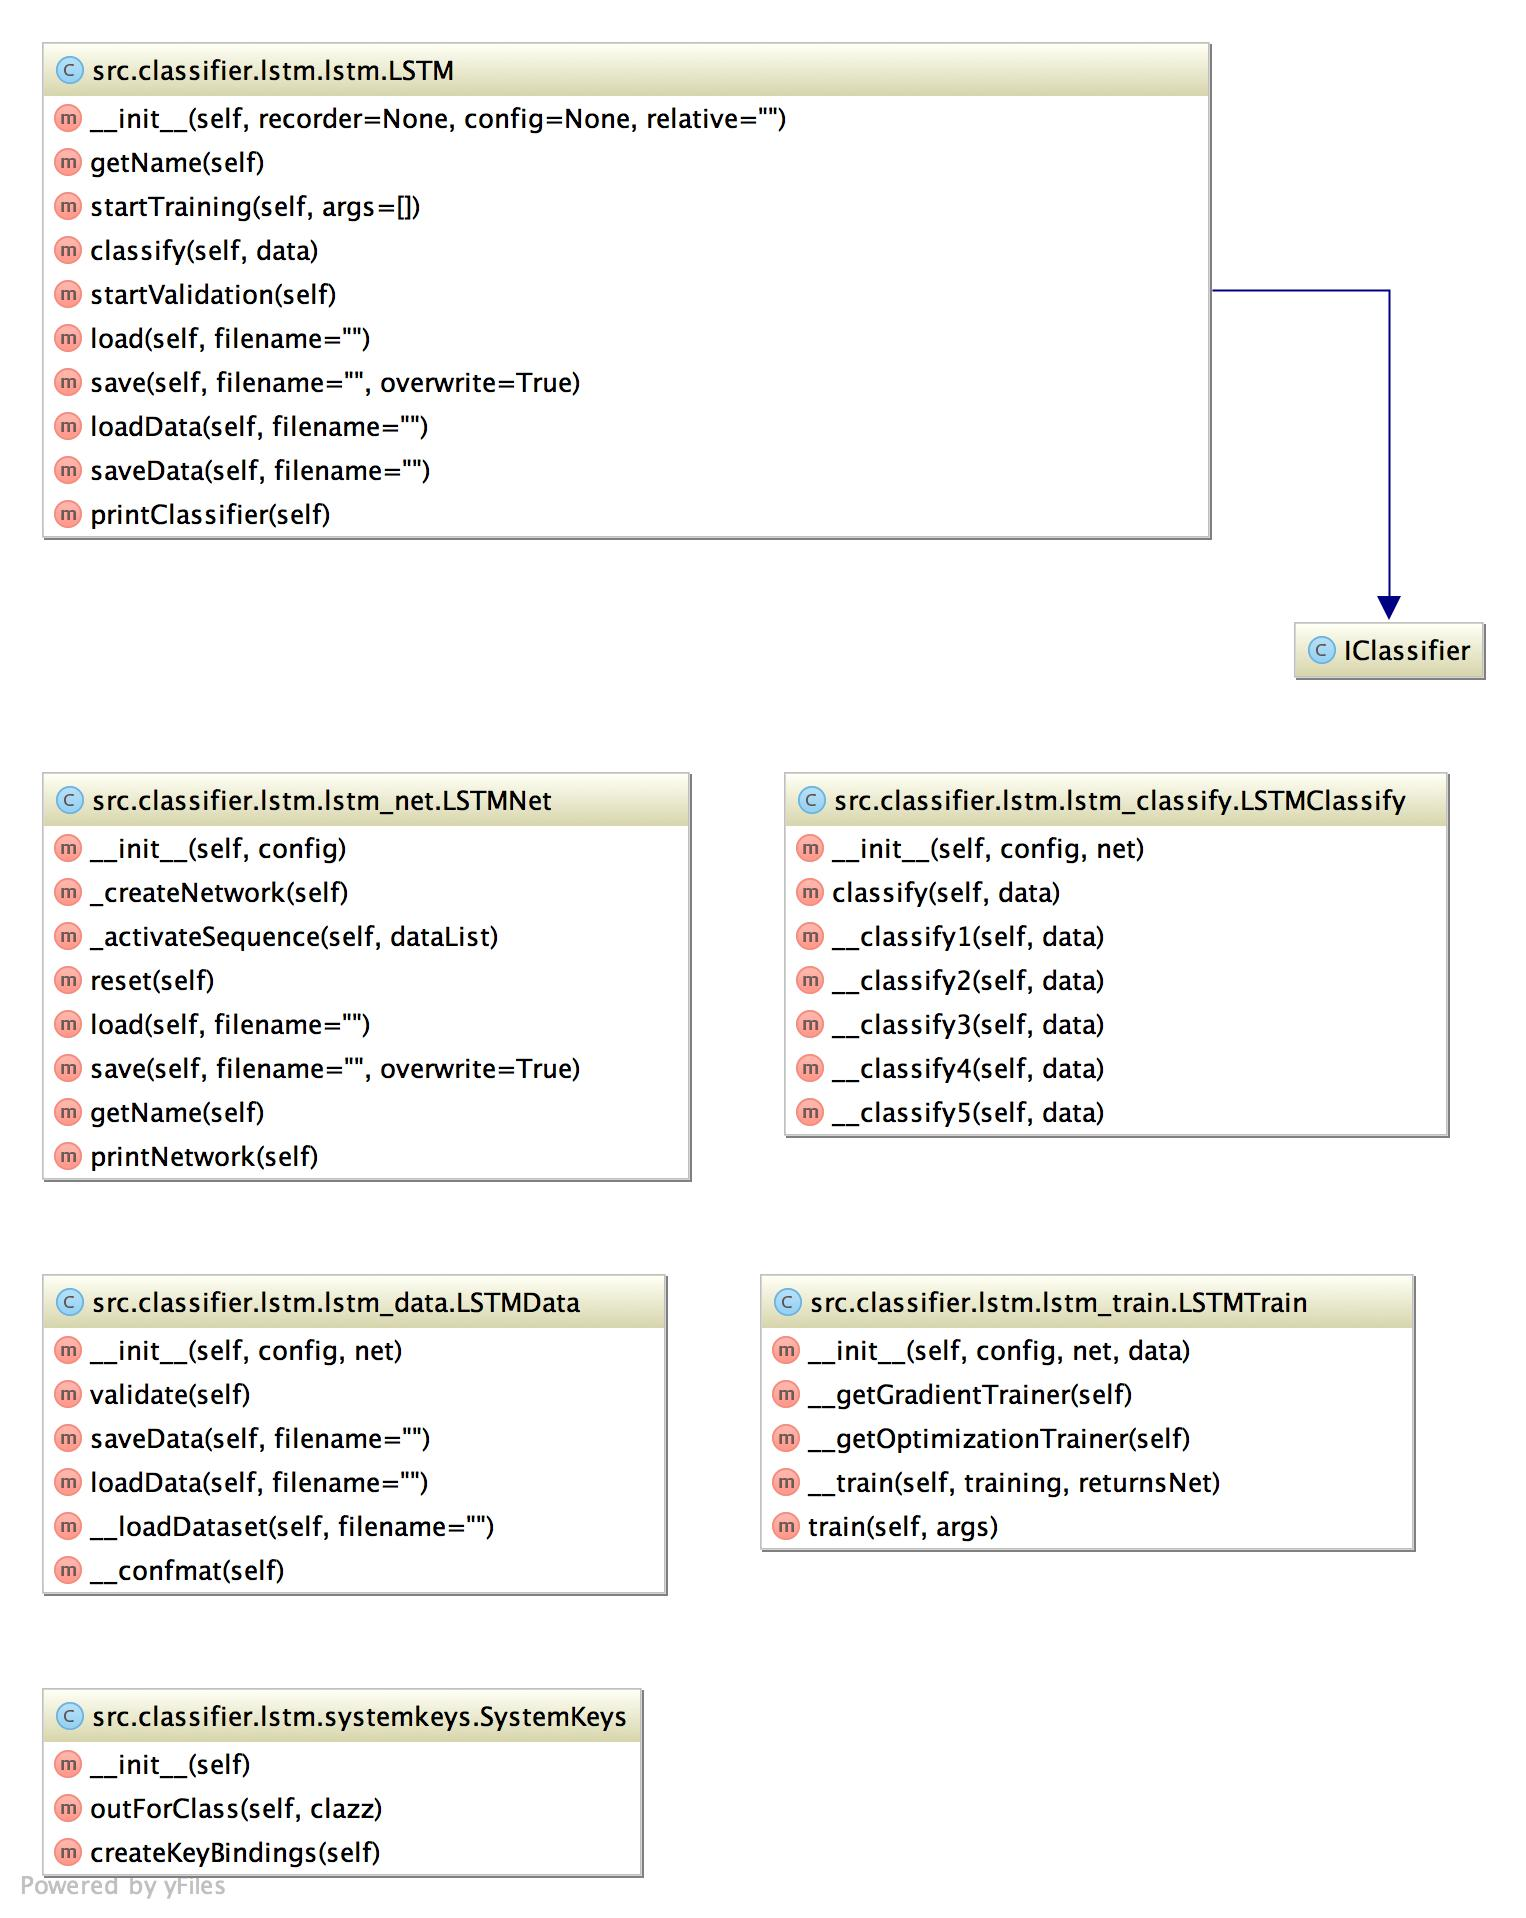
\includegraphics[width=0.95\textwidth]{lstm/diagram}
  \caption[\acs{LSTM} Klassendiagramm]{\acs{LSTM} Klassendiagramm}
  \label{fig:lstm_class}
  \end{center}
\end{figure*}  


\end{document}
